%%
%% This is the 2018 To The Moon Burner Flight Manual
%%
%% Inspirational documents:
%% 
%% http://playadelfuego.org/sites/default/files/www_print_may13_web_spread.pdf
%% http://alchemyburn.com/siteitemsep=.0125mm,parsep=2pts/default/files/Alchemy-2015-Survival-Guide.pdf
%% http://www.euphoriaburn.com/sites/euphoriaburn.com/files/docs/Euphoria-2016-SurvivalGuide.pdf
%% https://drive.google.com/open?id=17P6mr4Ru1PN8U_qDDtwwpvcRyxrh4A0x
%% 

% \documentclass[fontsize=8pt,twocolumn,titlepage=firstiscover,numbers=noenddot,DIV=16]{scrreprt}
\documentclass[fontsize=8pt,twocolumn,titlepage=firstiscover,numbers=noenddot,DIV=16]{scrreprt}

% specific formattinhg for pocket format
\usepackage[margin=0.5in]{geometry}
\geometry{
  paperheight=8.5in,
  paperwidth=5.5in,
  heightrounded,
}
\setlength{\footskip}{.3in}



\title{To the Moon Pocket Guide}

\author{Raptor, Piprrr}


%% Remove leading space in new paragraphs
\setlength{\parindent}{0pt}
%% Set space between paragraphs
\setlength{\parskip}{.7em}
%% Set space between columns
\setlength{\columnsep}{1.8em}
%% Penalize orphan lines at top and bottom of page
\widowpenalty 10000
\clubpenalty 10000


% moved usepackages into separate file
% file also has some other definitions, like the title page images etc.

% This defines a new TeX boolean 'isflight' that is true iff we're making the *flight* manual, not the preflight
\newif\ifisflight
% same but for the portapotties events list
\newif\ifisporto

% Type 1 fonts
\usepackage[T1]{fontenc}

% for emojii support

% trying for direct emoji support
\usepackage{fontspec}
\usepackage{fontawesome}
\usepackage{fontawesome5}

\newfontfamily\DejaSans{DejaVu Sans}

% Include figures
\usepackage{graphicx}

% For SI Units; mostly to use for degrees.
\usepackage{siunitx}

%multirow support for tables
\usepackage{multirow}

% For nice slanted fractions
\usepackage{xfrac}


% for TODO items
\usepackage[usenames,dvipsnames]{xcolor}
% \usepackage[disable]{todonotes}
\usepackage[]{todonotes}
%% green bubbles for BOD todos
\newcommand{\bod}[2][]{\todo[color=green,#1]{#2}}

% Fancy tables
\usepackage{booktabs}

% Allow for use of multiple columns
\usepackage{multicol}

% This provides a wee bit better typography
\usepackage{microtype}

% Some basic math 
\usepackage{calc}

% Make the labels for labeling lists look nicer with a sans serif font
\addtokomafont{labelinglabel}{\sffamily}

% This to grab the \square used in checklists
\usepackage{amssymb}

% Better lists
\usepackage{enumitem}

% Make a checklist environment
\newlist{checklist}{itemize}{2}
\setlist[checklist]{label=$\square$}

% \usepackage{libertine}
\renewcommand{\familydefault}{\sfdefault}

% For better appendix support
% TODO Not sure if we want appendices; overkill?
\usepackage{appendix}

% sideways figures
\usepackage{rotating}

% figures wrapped in text
\usepackage{wrapfig}

% % caption next to figure (SCfigure)
% \usepackage{sidecap}

% % another attempt to get caption next to image
% \usepackage{paracol}

% Glossary definitions and acronyms common to pre-flight manual and survival guide
%
% A list of glossary terms and acronyms
%
% Shared between pre-flight manual and survival guide
%

%%
%% Begin glossary stuff
%%
% \usepackage[acronym,style=long3colborder]{glossaries}
\usepackage[acronym]{glossaries}

\usepackage{glossary-longbooktabs}

% First use use full name of acronym, then the abbreviated.
\setacronymstyle{long-short}

% From https://en.wikibooks.org/wiki/LaTeX/Glossary#Defining_glossary_entries
% To support things that are both acronyms and glossary items, e.g., "MOOP."
\usepackage{xparse}
\DeclareDocumentCommand{\newdualentry}{ O{} O{} m m m m } {
  \newglossaryentry{gls-#3}{name={#5},text={#5\glsadd{#3}},
    description={#6},#1
  }
  \makeglossaries
  \newacronym[see={[Glossary:]{gls-#3}},#2]{#3}{#4}{#5\glsadd{gls-#3}}
}

% \makenoidxglossaries
\makeglossaries

% \newglossaryentry{moopgl}{
% name = {Matter Out of Place},
% description = {Anything not part of the natural environment, such as glitter, litter, bottle caps, and cigarette butts.}
% }

\newdualentry{moop} % label
  {MOOP}            % abbreviation
  {Matter Out of Place}  % long form
  {Trash, litter, things lost or left behind, things on the ground that should not be there.} % description
  

\newglossaryentry{rangers} {
name = {Rangers},
description = {A volunteer empowered to address safety concerns, mediate disputes, and resolve conflicts when they cannot be resolved by the persons involved}
% This is already in the team description for rangers
% \begin{labeling}{khaki}
% \item[alpha:] novice ranger
% \item[dirt:] (as in older than ...) an experienced ranger
% \item[khaki:] a Ranger that stays at HQ as a point-of-contact
% \end{labeling}}
}

\newglossaryentry{effigy} {
name = {effigy},
description = {The main art piece to be burned Saturday night.}
}

\newglossaryentry{graywater} {
name = {gray water},
description = {Water left-over from cleaning dishes or bathing.}
}

\newglossaryentry{crew} {
name = {crew},
description = {You.}
}

\newglossaryentry{gifting} {
name = {gifting},
description = {Giving food, an item, or a service without any expectation of reciprocity}
}

\newglossaryentry{mudburn} {
name = {Mud Burn},
description = {A burn characterized by extreme mud due to inclement weather}
}

\newglossaryentry{artcar} {
name = {Art Car},
description = {See: \gls{mutantvehicles}}
}

\newglossaryentry{mutantvehicles} {
name = {Mutant Vehicles},
description = {A motorized conveyance that is radically, stunningly, and safely modified. See also: \gls{artcar}}
}

\newglossaryentry{centercamp} {
name = {Center Camp},
description = {Host to many different musical experiences, performance art, and educational classes.}
}

\newglossaryentry{conclave} {
name = {Conclave},
description = {The Saturday night fire performance delivered by any interested and competent participants.}
}

\newglossaryentry{cockpit} {
name = {COCKpit},
description = {The main information station to visit when you have questions and need answers. There is also a huge map so you can find yourself. It's the home base for Volunteer Coordination, First Aid, \gls{lamplighters}, and \gls{lnt}}
}

\newglossaryentry{groundcontrol} {
name = {Ground Control},
description = {Department of Public Works Headquarters.}
}

\newglossaryentry{missioncontrol} {
name = {Mission Control},
description = {Rangers Headquarters.}
}

\newglossaryentry{shiftlead} {
name = {shift lead},
description = {some teams operator on a 24 $\times$ 7 schedule that is divided into shifts; a shift lead is one designated to be in charge of a given team for a shift}
}


\newglossaryentry{darkwad} {
name = {darkwad},
description = {Someone who is running around at night with no light or glow on. It gets dark out there. Real dark.}
}

\newglossaryentry{darksideofthemoon} {
name = {Dark Side of the Moon},
description = {Open camping located on the extreme eastern edge of the site well within the tree line.  Ideal for introverts without a theme camp, or those averse to the sun.}
}

\newglossaryentry{defaultworld} {
name = {default world},
description = {The rest of the world that is not a burn.}
}

% dual entry
\newdualentry{dmv} 
{DMV}
{Department of Mutant Vehicles}
{The volunteers who review and register \gls{mutantvehicles}, giving them permission to drive during the event.}


%dualentry
\newdualentry{dpw} 
{DPW}
{Department of Public Works}
{The team responsible for overseeing construction of the infrastructure, managing inventory, completing construction projects, overseeing Build Weekend and Tear Down, fueling the Effigy and Temple, and generally working behind the scenes during the event to deal with infrastructure issues as they arise. Also called Public Works.}

\newglossaryentry{education} {
name = {education},
description = {See: \glspl{greeter}}
}

\newglossaryentry{effigyburnfield} {
name = {Effigy Burn Field},
description = {This is where effigy and temple(s) get burnt.}
}

\newglossaryentry{eventleads} {
name = {event leads},
description = {This the team of volunteers who manage the event, and whom facilitate community needs. They are selected by the Board of Directors, which in turn is elected by the \gls{ttm} community.}
}

\newglossaryentry{gate} {
name = {Gate},
description = {The entrance to the burn where your ticket and ID will be checked, and where you will sign a waiver.}
}

\newglossaryentry{greeter} {
name = {Greeter},
description = {A friendly volunteer that will welcome you to the Burn, give you your \gls{swag}, and provide \gls{education} about the 10 (11) Principles. }
}

\newglossaryentry{groundscore} {
name = {ground score},
description = {\gls{moop} that is useful to you --- if you find something that someone dropped and you keep it, it's a ground score. If it looks valuable don’t be a dick, take it to lost and found. }
}

\newglossaryentry{lamplighters} {
name = {lamp lighters},
description = {The volunteer group that lights lanterns each night to illuminate some of the roads.}
}

\newglossaryentry{launchpad} {
name = {launchpad},
description = {Area where \gls{gate}/\glspl{greeter} are located.}
}

\newglossaryentry{temple} {
name = {temple},
description = {this is the art structure burned on the last night (though Euphoria has kindly donated their temple, which is to be burned Friday night)}
}

% dual entry
\newdualentry{lnt} 
{LNT}
{Leave No Trace}
{The concept that we should leave the property in better shape than we found it. It can also be verbed, as in ``Hey, I'm going to LNT the campsite after everyone packs up.'' }

\newglossaryentry{moonrangerstation} {
name = {Moon Ranger Station},
description = {Meeting point for Ranger Training.}
}

\newglossaryentry{opencamping} {
name = {open camping},
description = {where camping is permitted by participants who do not have a pre-assigned Theme Camp.}
}

\newglossaryentry{perimeter} {
name = {perimeter},
description = {Predetermined areas around the structure combustion events (Effigy, Temple, etc) that are staffed by volunteers to keep observers at a safe distance.}
}

% dual entry
\newdualentry{poop}
{POOP}
{Person Out of Place}
{People who are not where they should be. If you see someone passed out on the ground in the middle of the field, they may be drunk or having a medical emergency. Check and see if they are OK. If they want to be there, it's at their own risk if they get run over by a golf cart; but we try to get these people back to their camps.}

\newglossaryentry{sparklepony} {
name = {sparkle pony},
description = {A derogatory term for burners who show up to the event with little or no food or water, suitcases full of costumes and makeup, who do no work and no volunteering and only exist to look pretty, have fun, and party. They are often fashionably attired since they packed nothing but costumes.}
}

\newglossaryentry{swag} {
name = {swag},
description = {A memento from a burn, often wearable. You get swag for attending from \glspl{greeter}, often swag from your volunteer teams, and people you meet may gift you swag they made for the burn.}
}

\newglossaryentry{teamleads} {
name = {team leads},
description = {The people who head up each team that makes the burn happen.}
}

\newglossaryentry{tenprinciples} {
name = {Ten Principles},
description = {The ten core guiding concepts of most burns. }
}

\newglossaryentry{themecamp} {
name = {theme camp},
description = {A group of people camping together in a pre-assigned spot who often have common bonds and shared activities.}
}

\newglossaryentry{tbass} {
name = {Tranquility Base},
description = {(A.k.a., Tbase/Sanctuary) A dedicated space for those who may need an environment or area in which to better acclimate or adjust to the Burn.}
}

\newglossaryentry{village} {
name = {village},
description = {A group of Theme Camps sharing a common space and ethos.}
}

\newglossaryentry{eleventhprinciple} {
name = {11th Principle},
description = {The 11th Principle}
}


\newglossaryentry{preflightmanual} {
name = {pre-flight manual},
description = {The document that contains information essential for planning and preparing for \gls{ttm}}
}


\newglossaryentry{survivalguide} {
name = {survival guide},
description = {The document that contains information essential for planning and preparing for \gls{ttm}, and which provides information about events, theme camps, and art during the event.  Essentially, it is the \gls{preflightmanual} plus art, camp, and event listings.}
}


\newglossaryentry{parking} {
name = {Parking},
description = {There is a large parking area at the entrance.}
}

%% Glossary item template
% \newglossaryentry{} {
% name = {},
% sort = {},
% description = {}
% }

%% Glossary dual entry template -- i.e., things that are acronyms *and* glossary entries, like MOOP
% \newdualentry{OWD} % label
%   {OWD}            % abbreviation
%   {One-Way Delay}  % long form
%   {The time a packet uses through a network from one host to another} % description

\setglossarysection{subsection}


% acronym tag, short name, long name
\newacronym{ttm}   {TTM}      {To the Moon}
\newacronym{bod}   {BOD}      {Board of Directors}
\newacronym{leo}   {LEO}      {Law Enforcement Officer}
\newacronym{vc}    {VC}       {Volunteer Coordination}
\newacronym{gtfio} {GTFIO}    {Get the Fuck In and Out}
\newacronym{love}  {L.O.V.E.} {Lunar Orbit Vehicle Extraction}
\newacronym{pipo}  {PIPO}     {Pack in/pack out}
\newacronym{el}    {EL}       {Event Lead}
% \newacronym{SHORTNAME}  {ABBREV}  {LONGNAME}



%%
%% End glossary stuff
%%



% set text in a shape
\usepackage{shapepar}

% add H placement option for floats which really puts them where you want them
% \usepackage{float}
\usepackage{floatrow}

% absolute position for text (titlepage)
\usepackage[absolute]{textpos}
 \setlength{\TPHorizModule}{1mm}%
 \setlength{\TPVertModule}{1mm}%

% sideways figure/"H" placement 
\usepackage{float}

% This is for fancy schmancy ornaments
\usepackage{pgfornament}
\usepackage{tikz}
\usetikzlibrary{calc,matrix,shapes}

%%
%% For setting the title page background
%%
\usepackage{eso-pic}

%% fancy table alignment, used to create formatting for headers in events and camps with icons
\usepackage{tabularray}
\SetTblrInner{colsep=0pt}

% \usepackage{tasks}

\definecolor{red2022}{HTML}{C0062C}

\newcommand\LetterSizeTitlePic{%
\put(0,0){%
\parbox[b][\paperheight]{\paperwidth}{%
\vfill
\centering
{\includegraphics[width=\paperwidth,height=\paperheight]{images/cover-art/2022coverpageletter}}%
\vfill
}}}

\newcommand\HalfLetterSizeTitlePic{%
\put(0,0){%
\parbox[b][\paperheight]{\paperwidth}{%
\vfill
\centering
\includegraphics[width=\paperwidth,height=\paperheight]{images/cover-art/2022coverpageHalfLetter}%
\vfill
}}}

% NASA image from https://svs.gsfc.nasa.gov/vis/a000000/a003600/a003686/SPflyover_v07_still.5000.jpg
\newcommand\ThemePic{%
\put(0,0){%
\parbox[b][\paperheight]{\paperwidth}{%
\vfill
\centering
% 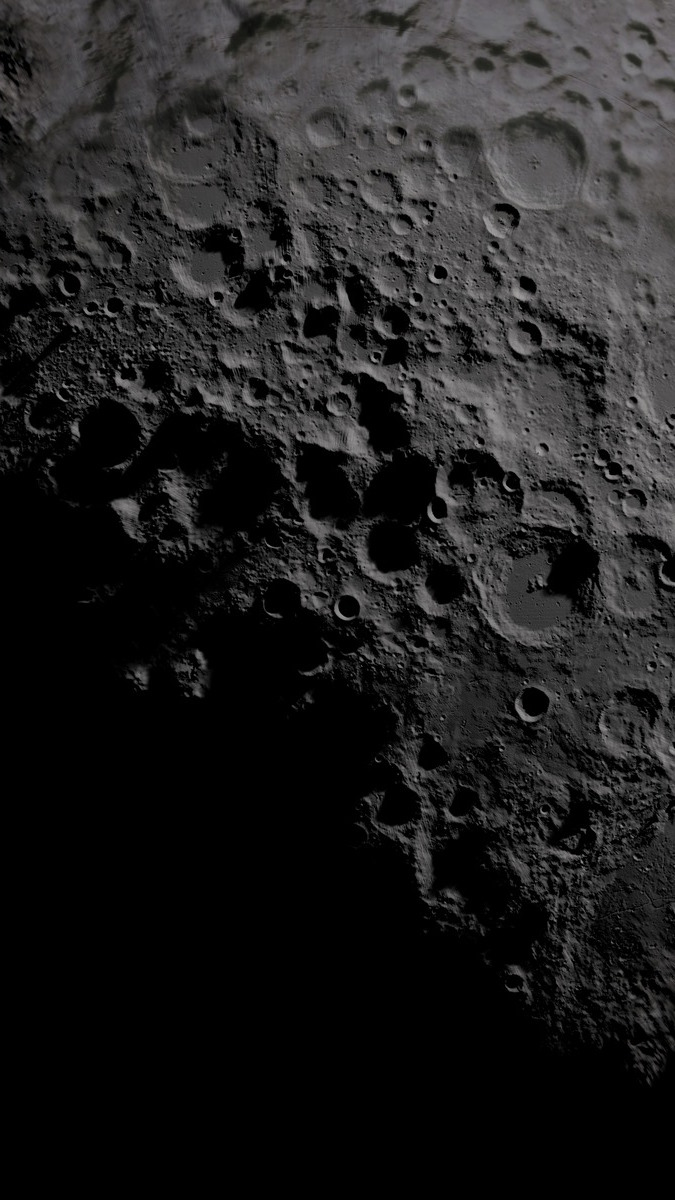
\includegraphics[width=\paperwidth,height=\paperheight]{images/moon_bg.jpg}%
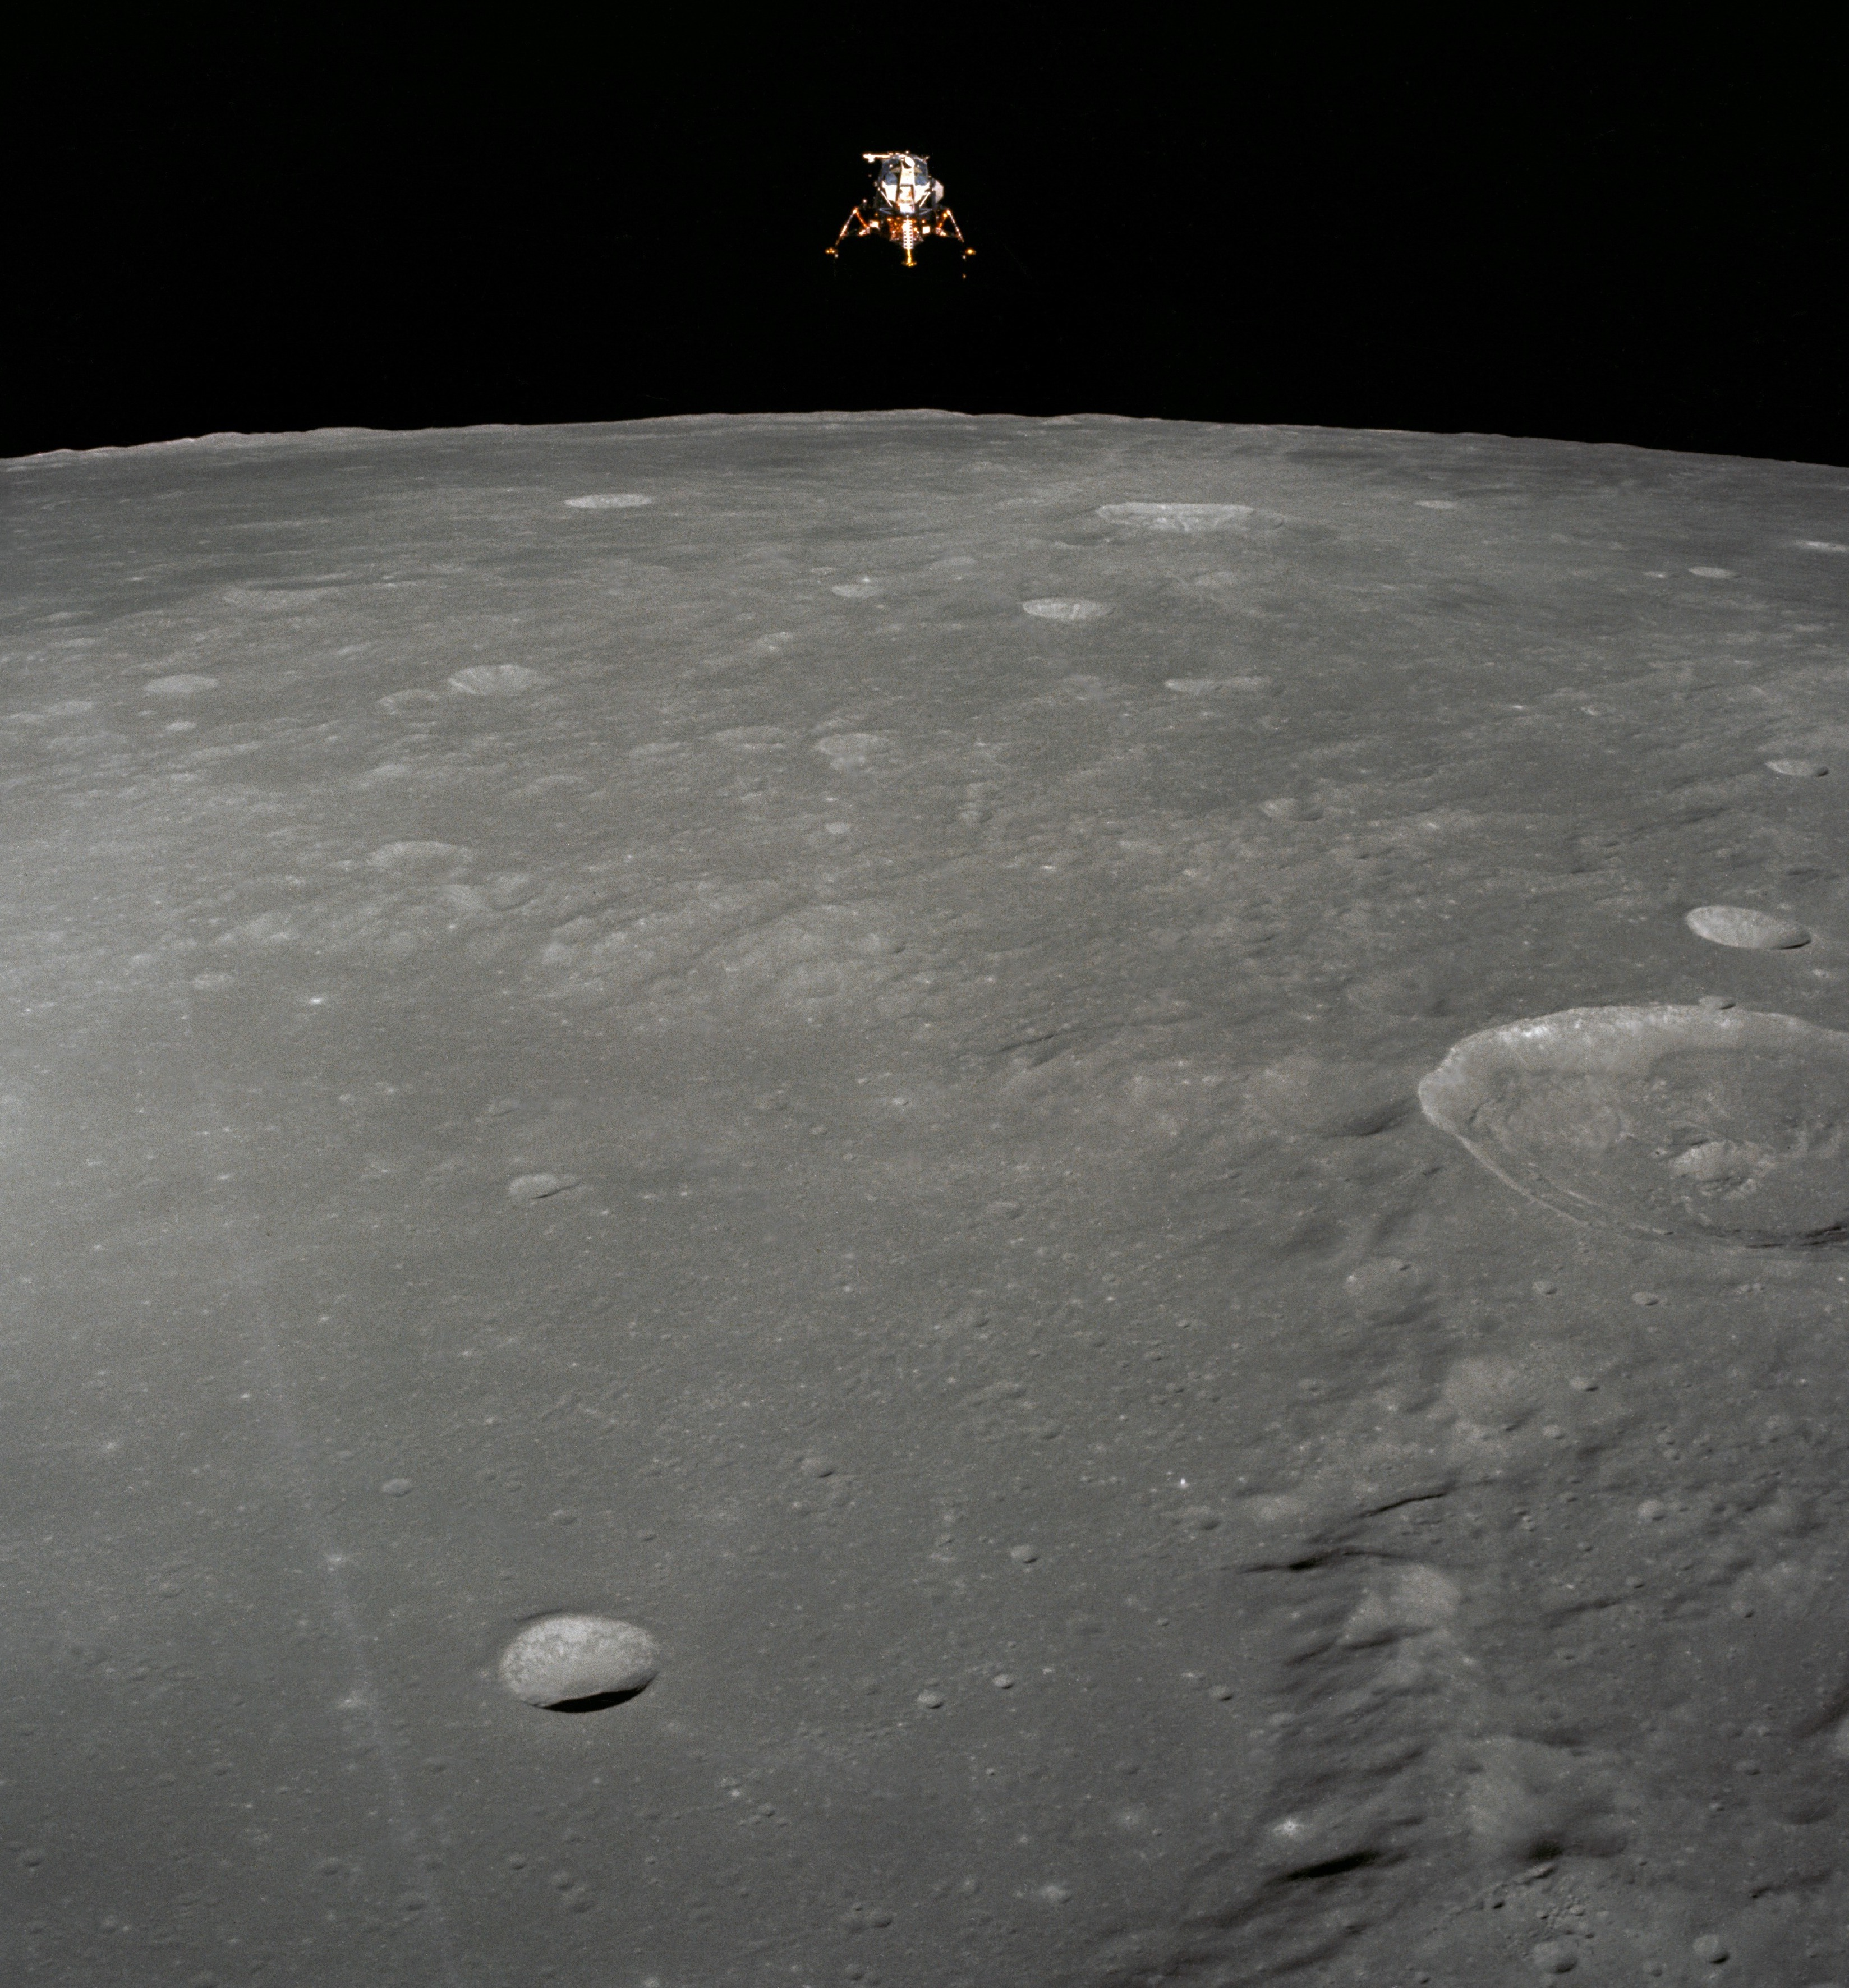
\includegraphics[width=\paperwidth,height=\paperheight]{images/cover-art/landercroppedmore.jpg}%
\vfill
}}}

%% Consistent notation for am and pm, easy to change right here :D
\usepackage{xspace}
\newcommand{\am}{am\xspace}
\renewcommand{\pm}{pm\xspace}

% Support for URLs and document links
\usepackage[]{hyperref}
% \hypersetup{colorlinks=true,allcolors=[rgb]{0,.5,.7}}
\hypersetup{
  colorlinks   = true, %Colours links instead of ugly boxes
  urlcolor     = [rgb]{0,.5,.7}, %Colour for external hyperlinks
  linkcolor    = [rgb]{0,.5,.7}, %Colour of internal links
  citecolor   = [rgb]{0,.5,.7} %Colour of citations
}
% \hypersetup{colorlinks=false}


%% Remove leading space in new paragraphs
\setlength{\parindent}{0pt}
\setlength{\parskip}{.7em}
\widowpenalty 10000
\clubpenalty 10000



\frenchspacing % eliminate extra spaces after periods

% \newcommand{\ttmfont}[1]{\fontsize{2.3cm}{1cm}\selectfont{\textbf{\textcolor{red2022}{\sffamily#1}}}}
% \newcommand{\guidetypefont}[1]{\fontsize{1.2cm}{1.4cm}\selectfont{\textbf{\textcolor{red2022}{\sffamily#1}}}}
% \newcommand{\guideversionfont}[1]{\fontsize{.95cm}{1.3cm}\selectfont{\textcolor{red2022}{\sffamily#1}}}
% \newcommand{\locationfont}[1]{\fontsize{0.6cm}{.5cm}\selectfont{\textbf{\textcolor{red2022}{\sffamily\uppercase{#1}}}}}


% Can't get this to work right
% \usepackage[]{thumbs}

% \usepackage{chapterthumb}
% \newrobustcmd{\SetChapterThumbHeader}{%
% \lohead[\putchapterthumb]{\putchapterthumb}%
% }%

% \newrobustcmd{\ClearChapterThumbHeader}{%
% \lohead[]{}%
% }%

% \newrobustcmd{\refcommand}[1]{%
% \nameref*{#1}%
% }%

% \newtoggle{UseChapterThumb}%
% \toggletrue{UseChapterThumb}%

% \renewcommand*{\chapterthumbformat}{\refcommand{chapter::title::\number\value{chapter}}}%

% \makeatletter

% \newcounter{totalchaptercounter}%

% \newrobustcmd{\CreateUniqueChapterLabel}[1]{% Well, `unique` as it can be ;-)
% \refstepcounter{totalchaptercounter}%
% \label{chapter::title::\number\value{totalchaptercounter}}%
% }%

% \let\LaTeXStandardChapter\chapter%

% \newcommand{\chapter@noopt}[1]{%
% \iftoggle{UseChapterThumb}{\SetChapterThumbHeader}{\ClearChapterThumbHeader}
% \LaTeXStandardChapter{#1}%
% \CreateUniqueChapterLabel{#1}% Must appear after chapter title is done
% }%

% \newcommand{\chapter@opt}[2][]{%
% \iftoggle{UseChapterThumb}{\SetChapterThumbHeader}{\ClearChapterThumbHeader}
% \LaTeXStandardChapter[#1]{#2}%
% \CreateUniqueChapterLabel{#2}% Must appear after chapter title is done
% }%


% \newcommand{\unstarredchapter}{%
% \@ifnextchar[{\chapter@opt}{\chapter@noopt}%
% }%

% \newcommand{\starredchapter}[1]{%
% \ClearChapterThumbHeader% Clear the headers -> no chapterthumb here 
% \LaTeXStandardChapter*{#1}%   
% }%

% \renewcommand{\chapter}{%
% \@ifstar{\starredchapter}{\unstarredchapter}%
% }%


% Yes, we are in "flight manual mode", so enable those tweaks; this variable defined in preamble
\isflighttrue

\newcommand{\ttmfont}[1]{\fontsize{1.4cm}{1cm}\selectfont{\textbf{\textcolor{red2022}{\sffamily#1}}}}
\newcommand{\guidetypefont}[1]{\fontsize{0.8cm}{1.4cm}\selectfont{\textbf{\textcolor{red2022}{\sffamily#1}}}}
\newcommand{\guideversionfont}[1]{\fontsize{.6cm}{1.3cm}\selectfont{\textcolor{red2022}{\sffamily#1}}}
\newcommand{\locationfont}[1]{\fontsize{0.4cm}{.3cm}\selectfont{\textbf{\textcolor{red2022}{\sffamily\uppercase{#1}}}}}

\begin{document}



\begin{titlepage}
%% drop in the image for the title page
\AddToShipoutPicture*{\HalfLetterSizeTitlePic}

% set text in front of image
\ttmfont{~}\\
\vspace{5.2cm}

\hspace{1.7cm}\ttmfont{To The Moon}

% \vspace{-0.1cm}

\hspace{1.7cm}\guidetypefont{Pocket Guide}

\vspace{-0.4cm}

\hspace{1.7cm}\guideversionfont{Final --- June 19, 2022}

\vspace{4.2cm}

\hspace{1.7cm}\locationfont{Catoosa Event Center}

\hspace{1.7cm}\locationfont{Allardt, Tennessee}

\vspace{-1cm} % to pull up the inner cover to where it belongs

\hspace{1em} %required to push the content of the next page out of this one
\end{titlepage}

% \maketitle not needed because we're using a titlepage environment
% \maketitle

%\AddToShipoutPicture*{\OtherBackgroundPic}

% This is true if only doing the flight manual, not the pre-flight
\ifisflight
  % This one page needs to be one column to look right, even
  % in the flight manual, proper.
  \onecolumn
\else 
  % Doesn't seem to do anything for the chapter heading in flight manual.  Wah.
  \vspace{-1cm}
\fi

% Note that this chapter heading is a little high up on the flight manual, but is great on PFM.
% It may not be worthwhile fixing since we have bigger fish to fry. -- Piprrr
\chapter*{\centering \textbf{\textcolor{white}{History of Mysteries}}}
\label{sec:theme}


% \begin{center}
% \pgfornament[width = .5\textwidth,color = white]{88}
% \end{center}



%% And now drop in the image for the title page
\AddToShipoutPicture*{\ThemePic}

\ifisflight
  \vspace{1cm}
\fi

\textbf{\textcolor{white}{Humanity on Earth is riddled with a long history of mysterious events, monuments, legends, folklore and puzzles. For centuries we have centered our science, art and religion on concepts and ideas that elude our present cognition. Were extraterrestrials perceived as gods? What technology was available for constructing things like the pyramids and Stonehenge? What happened to the Mayan civilization? Where is Atlantis?}}

\textbf{\textcolor{white}{What we cannot answer on this planet may be revealed on  the dark side of the Moon. This lunar landing is no myth... We can prove it. Join in this year's lunar voyage to reveal or to just revel in our History of Mysteries.}}

\textbf{\textcolor{white}{If we build a pyramid on the moon, can we complete the energetic grid? Can we finally communicate with aliens by building our own crop circles? Is this a maze to the center of consciousness or just a historical rabbit hole which only reveals more questions? Is the answer to the universe really 42? Were unicorns real? Could you pass the Sphinx's riddle? Maybe the Clinch River really is the fountain of youth!}}

\textbf{\textcolor{white}{There are two things that could happen when diving deep into solving some of these mysteries. Either we uncover some new truths, new languages, new rituals, or we create even more mysteries, mazes, puzzles and traps. Choose your own adventure.}}

\textbf{\textcolor{white}{This year’s art theme will illuminate our most ancient questions, visions and anomalies, sacred geometry and secret mythologies.}}


\begin{center}
\pgfornament[width = .5\textwidth,color = white]{88}
\end{center}

\vspace{1pt}

\begin{multicols}{2}
\begin{centering}
\textbf{\textcolor{white}{Build a maze,\\
or\\Bust a myth\\
Solve the riddle\\
Leave with more questions than you arrived with}}

% \columnbreak

\textbf{\textcolor{white}{The world will soon know what rests\\
on the dark side of the moon\\
Only for a fleeting moment will all be revealed}}

% \columnbreak

\textbf{\textcolor{white}{In the flames of our odyssey\\
History will be made history once again\\
And the mysteries will remain\\
To be told merely as stories of what happened when we\\
journeyed across the universe and... \\}}
\end{centering}

\begin{flushright}
\textbf{\textcolor{white}{...To The Moon}}
\end{flushright}

\end{multicols}

\ifisflight
  \twocolumn
\fi

% \cleardoublepage


\tableofcontents

% \pagestyle{useheadings}

% \listoftodos

% include the introductory stuff
%
% This chapter provides history of TTM and gives the nod to volunteers and
% supporting organizations
%

\chapter[Welcome]{Welcome to the Moon, Traveler!!!}

% Welcome 

% What is To the Moon?
% History?
% This is true if only doing the flight manual, not the pre-flight
\ifisflight
  % This one page needs to be one column to look right, even
  % in the flight manual, proper.
  % failed experiment to add thumb guides
%   \addthumb{Welcome}{}{white}{black}
\putchapterthumb
\fi

\section*{Mission}
A Burn is a  multi day art and music camping event the intent of which is to build like minded community and to share:
your time, food, gifts, art, love, toys, and talents and participate in creating something in the process that inspires beyond measure.

"A unique and distinctive culture emerges from "The Burning Man" Experience. Rooted in the values expressed by the Ten Principles, this culture is manifested around the globe through art, communal effort, and innumerable individual acts of self expression. To many, it's a way of life." -Burning Man

\subsection*{To The Moon}
Burns reconnect one to their inner child and Merkabah, the divine light vehicle used to tune into the far realm of possibility and innovation.

Embark with us on a journey to the outer rims of creativity, art, music, and community as we initiate a collective experience geared towards positive transformation, endless inspiration, and participatory
co-creation. Bring your SELF, your talents, your radical self-expression, and your stardust TO THE MOON and back as we travel together further than our own imagination. You get out of it what you put int.

Simply put, we play with fire and run with scissors in a space shaped by our fantasy and that which is conjured up by our inspiration and elbow grease.... the sky is the limit. 

\subsection*{...And Back}
Art, Participation, Fire Play, Music and so much more motivate this 
community to build a temporary dwelling in which there is no stranger nor are there spectators. Everybody pitches in and brings something to the table.  
We stare at the clouds, dream in dust, set fire to the rain and howl at the moon.  

A Burn is an incredible way of learning firsthand the experience of the Whole being greater than the sum of its parts.  

It's a place where participants gather to celebrate self-expression and community who happen to know how to throw a party.  They conceive and build interactive theme camps, art installations, mutant vehicles, costumes and performances, and they gift them for the benefit and enjoyment of each other!

Art Camps, Theme Camps, Sounds Camps all are an integral part and at the heart of this experience.  The event comes to a climax with the burning of the Effigy Saturday night, and usually ends after Sunday's Temple Burn. 

The culture rallies around causes and activism from local art exhibits to food and coat drives to Burners Without Borders - spearheading change, inspiring involvement and making a splash! 

"In Dust we trust....."


\vspace*{\fill}
\begin{figure}[!h]
\centering
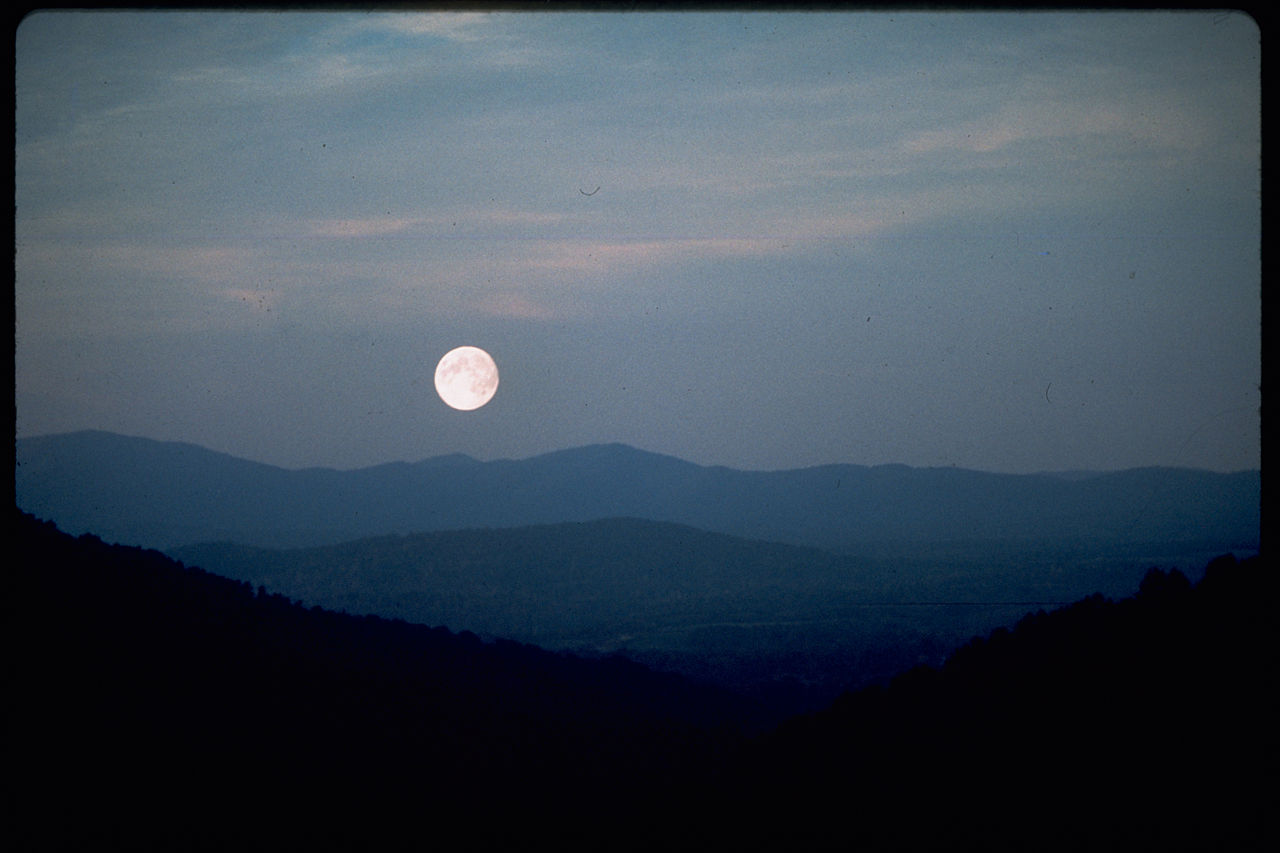
\includegraphics[width=.8\textwidth, trim=10 0 50 0, clip]{images/ShenandoahMoon}
% \caption{}
\label{image:mountainmoom}
\end{figure}
\vspace*{\fill}


% All things site, like directions, site maps, such as parking and (un)available amenities, checklist for packing
\chapter{In-Flight Procedures}

% This is true if only doing the flight manual, not the pre-flight
\ifisflight
  % This one page needs to be one column to look right, even
  % in the flight manual, proper.
  % failed experiment to add thumb guides
%   \addthumb{Welcome}{}{white}{black}
\putchapterthumb
\fi


Once you're at \gls{ttm}, you'll want to keep gate hours in mind (if you leave), and before you finally pack up to go to your rest-of-the-year home, please take a moment to read through our takeoff procedure!

\section*{Gate Hours}

\textbf{No vehicles will be allowed in after sunset! No moving vehicles \textit{period} inside the burn when it's dark - so if you get there right before sunset, you better get in, unload your stuff, and get right back out to parking ASAP. This is for the safety of everyone at the burn!}

Any vehicles that arrive after sunset will be redirected to parking, where we may or may not have a golf cart to help you carry some stuff in --- but don't count on it --- use that Radical Self-Reliance!

\begin{table*}[h!]
\footnotesize
\centering
\caption{\Gls{ttm} \gls{gate} hours}
\label{tbl:gatehours}
\begin{tabular}{@{}lll@{}}
\toprule
Wednesday & 6/12/2019 & 12--10\pm EST                                    \\ 
          &           & Theme Camp Early Entry Only w/ Pre-Registration \\
Thursday  & 6/13/2019 & 10\am--12\am EST                                   \\
Friday    & 6/14/2019 & 10\am--12\am EST                                    \\
Saturday  & 6/15/2019 & 10\am--6\pm EST, no admission after 6pm for rest of event \\
Sunday    & 6/16/2019 & 10\am--6\pm EST                                    \\
          &           & Departing Only                                  \\
Monday    & 6/17/2019 & 8\am--12\pm EST                                    \\
          &           & Departing Only                                  \\ \bottomrule
\end{tabular}
\end{table*}

\section*{Re-entry Procedure}

\textbf{There is no after hours entry without pre-arranged permission.  Crew arriving at the site outside gate operating hours will be turned away.  No crew is permitted to wait on the property until the gate opens.}

Please contact the \gls{bod} via \url{connect@tothemooonburn.com} well in advance of the event to work out options if long-distance travelers cannot arrive while the gate is open.

For the safety of other patrons and to preserve the integrity of the experience, \textbf{no} coming and going at leisure is allowed after checking in.  Exiting and returning \gls{ttm} are reserved \textbf{for medical and emergency reasons only}, and must be communicated to and cleared by the Gate Lead prior to leaving.

Theme Camp supply runs are possible Wednesday -- Friday before 10\pm \textbf{only}. Before leaving, \textbf{check at the gate} if a pass is needed. The Gate will check with \Gls{el} on call and a re-entry lanyard will be issued at \gls{el} discretion.

% If you forget something and need to ``make a run to the store'' talk to a team / event  / gate lead and we can grant Re-Entry if you combine your trip with one beneficial \gls{ttm} and the community at large.

\section*{Takeoff Procedure}
\subsection*{Leave No Trace}
\Gls{ttm} follows the \gls{lnt} principle (see \gls{tenprinciples}, page \pageref{tenprinciples}). Please take all your belongings, trash, and \gls{graywater} with you and leave the site in a better shape than you found it.

\subsection*{Takeoff Launch Window}

\Gls{ttm} officially closes at 11:59\pm EST, Sunday, June 17th.  All crew must vacate the site by 12pm EST, Monday, June 18th unless given explicit prior permission from Theme Camp Late Departure.

Vehicles can be driven on site on Monday to pack up. In case of inclement weather, a no driving / limited access policy to site will be implemented. Be prepared by bringing your own cart / wagon to transport gear out and to your vehicle.
\Gls{love} will be able to assist with shuttling gear to parking. 
Vehicles can \textbf{not} be parked alongside road to do so, but only be lined up at gate about 10 at a time.

Pleases look for announcements at \Gls{cockpit} / \Gls{gate}, as this policy may slightly change, depending on situation. 

\newpage
\section*{Resources}

% \begin{wrapfigure}{R}{0.3\textwidth}[h!]
% \centering
% 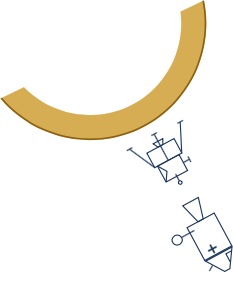
\includegraphics[width=0.25\textwidth]{images/landing1.png}
% % \caption{}
% \end{wrapfigure}
% \begin{multicols}{2}
\subsection*{Showers}
There are no showers. To keep yourself clean, bring wet wipes or biodegradable soap.
Please don't clean your dishes or yourself in the river since there are mussels in the river that are protected wildlife.  (And these are also the reason you should wear river shoes while in the river as the mussels will cut you. They're mean that way.)

\subsection*{Ice}
Ice will be soled from noon to 3 \pm every day for \$2 per 10 lbs bag.  Cash only! Bring small bills please. 


\subsection*{Lost and Found}
The Lost and Found will be at the \gls{cockpit} / \gls{vc} station.

\subsection*{Port-a-Potties}
There are Port-a-Potties on-site. Please don't put anything other than one-ply toilet paper and human waste in the Port-a-Potties. You will find Port-a-Potties in multiple locations across the site.



% \reflectbox{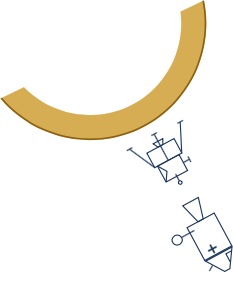
\includegraphics[width=\columnwidth,angle=180]{images/landing1.png}}

% \vspace*{\fill}
\ifisflight
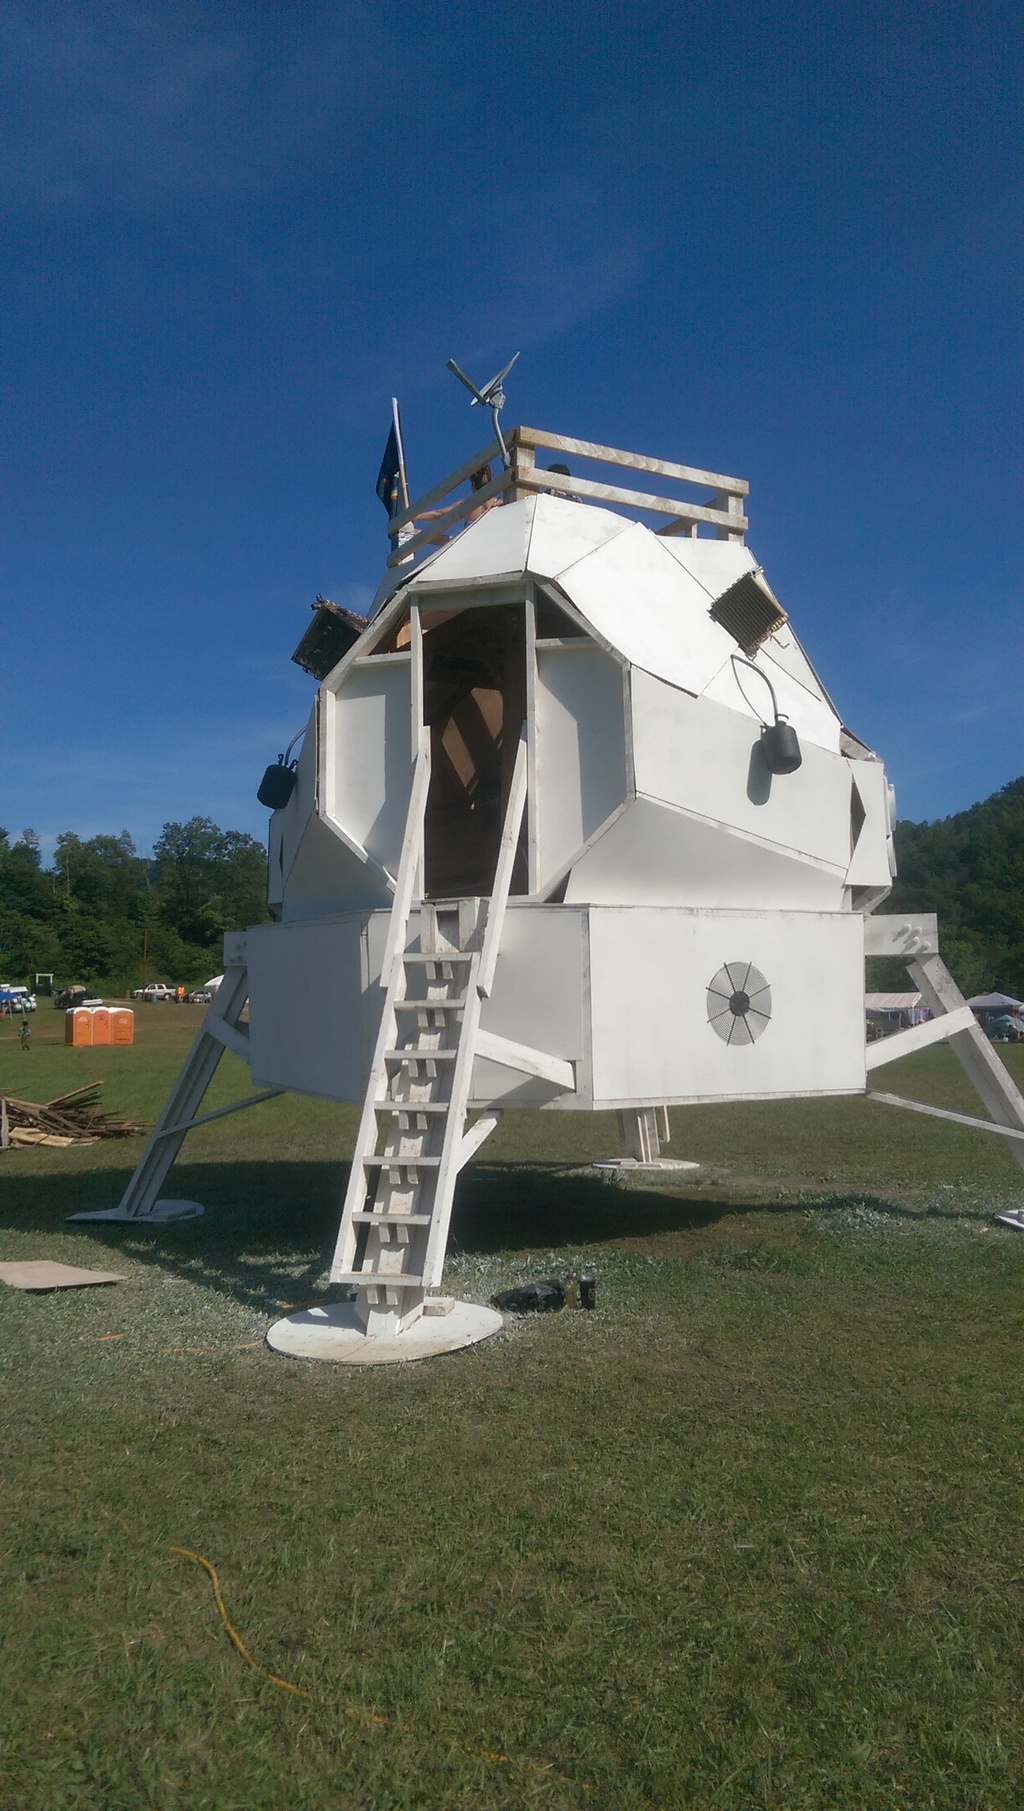
\includegraphics[width=\columnwidth]{images/2017Effigy_small.jpg}
\fi

% include vital info about participating in the burn, like guidelines, 10 principles and such
%
% This contains critical information regarding the burn, things like location,
% where the nearest hospital is located, definitions of terms, acronyms, the rules, 
% and information on any other burn-related resources.


\chapter{Astronaut Training}

% This is true if only doing the flight manual, not the pre-flight
\ifisflight
  % This one page needs to be one column to look right, even
  % in the flight manual, proper.
  % failed experiment to add thumb guides
%   \addthumb{Welcome}{}{white}{black}
\putchapterthumb
\fi

\section*{Guidelines}
We have few rules and kindly ask you to follow them, for your safety and those around and with you.  Look at them as a compass to orient yourself by while drifting in the orbit of this event. 

\subsection*{Safety}
Safety is our number one concern and breaching perimeter is a \textbf{serious} offense we will handle swiftly. 

\subsubsection*{Fire Safety}
\begin{itemize}[noitemsep]
\item \textbf{\textcolor{red}{If you breach effigy or temple perimeter, you will be removed from the property immediately -- no questions asked!}} 
\item No open ground and / or unattended fires. They must be contained and off ground. Please bring a fire bowl for this purpose. If you see a fire that is unattended or out of control, contact a Ranger immediately.
\end{itemize}

\subsubsection*{River Safety}
\begin{itemize}[noitemsep]
  \item Children under 13 must wear a flotation device.
  \item Children under 13 must wear water shoes (water shoes are highly recommended for  \textbf{Anyone} for added safety and traction, especially if caught in a current).
  \item All minors must be accompanied by a parent or legal guardian when in the water.
  \item \textbf{Anyone caught committing the below two actions will be ejected from the burn immediately:}
  \begin{itemize}[noitemsep]
    \item No jumping or diving off the bank into the river.
    \item No swimming after dark.
  \end{itemize}
\end{itemize}

% \begin{figure}[H]
% \centering
% 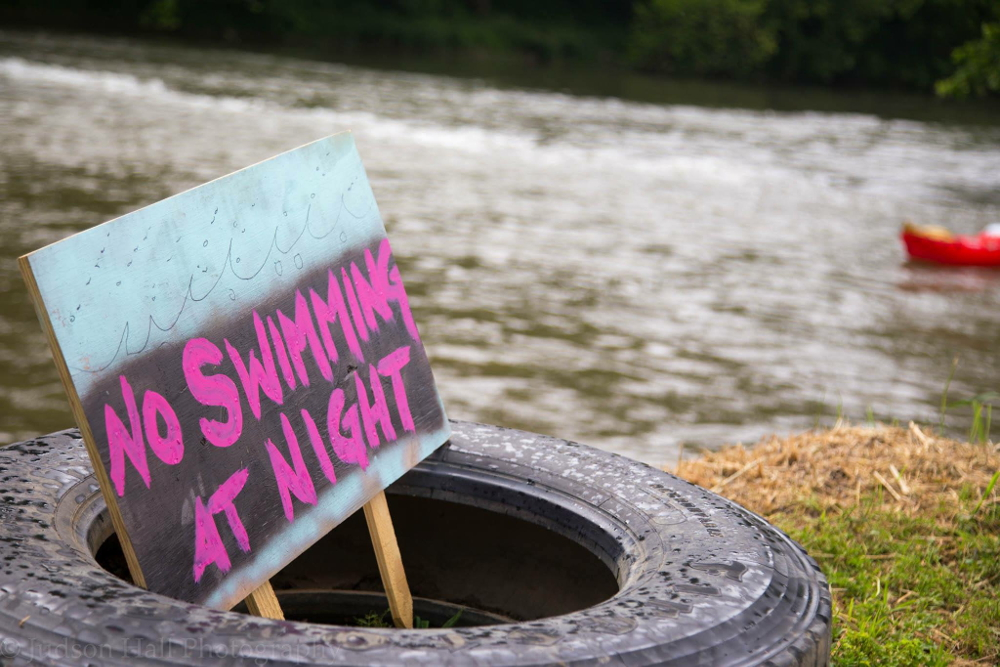
\includegraphics[width=.3\textwidth]{images/riversafety.jpeg}
% \caption{No swimming at night. Image courtesy of Judson Hall Photography, 2016.}
% \label{fig:2016riversafety}
% \end{figure}

% \clearpage
\subsection*{No Pets}
\label{sub:nopets}

Spirit Crossing has a \textbf{no pet} policy!
%
Should you need a service animal’s assistance to safely navigate our premises, please let us know at the gate.  A ``service animal'' is a dog (or other animal) individually trained to do work or perform certain tasks for a person with a disability.

Please be prepared to answer the following two questions so we may better determine at our discretion if your animal falls under the Service Animal Category, and in order for us to be in compliance with ADA regulations:
%
\begin{itemize}[noitemsep]
\item Is the service animal to the direct benefit of the disability?
\item What tasks and what work is the animal trained to perform in direct relation to the disability? 
\end{itemize}
 
% If your animal falls under one of the following categories, you will not be able to bring it into the festival grounds.

% Service Animals are \textbf{not}:
% \begin{multicols}{2}
% \begin{itemize}[noitemsep]
%   \item emotional support animals
%   \item therapeutic animals
%   \item companion animals
%   \item comfort animals
%   \item service animals in training
% \end{itemize}
% \end{multicols}

For your convenience, Scooby Shack Kennel is 20 minutes from Sneedville and can be reached at 423-921-0611.

Thank you for your cooperation and understanding!

% \begin{figure}[H]
% \centering
% 	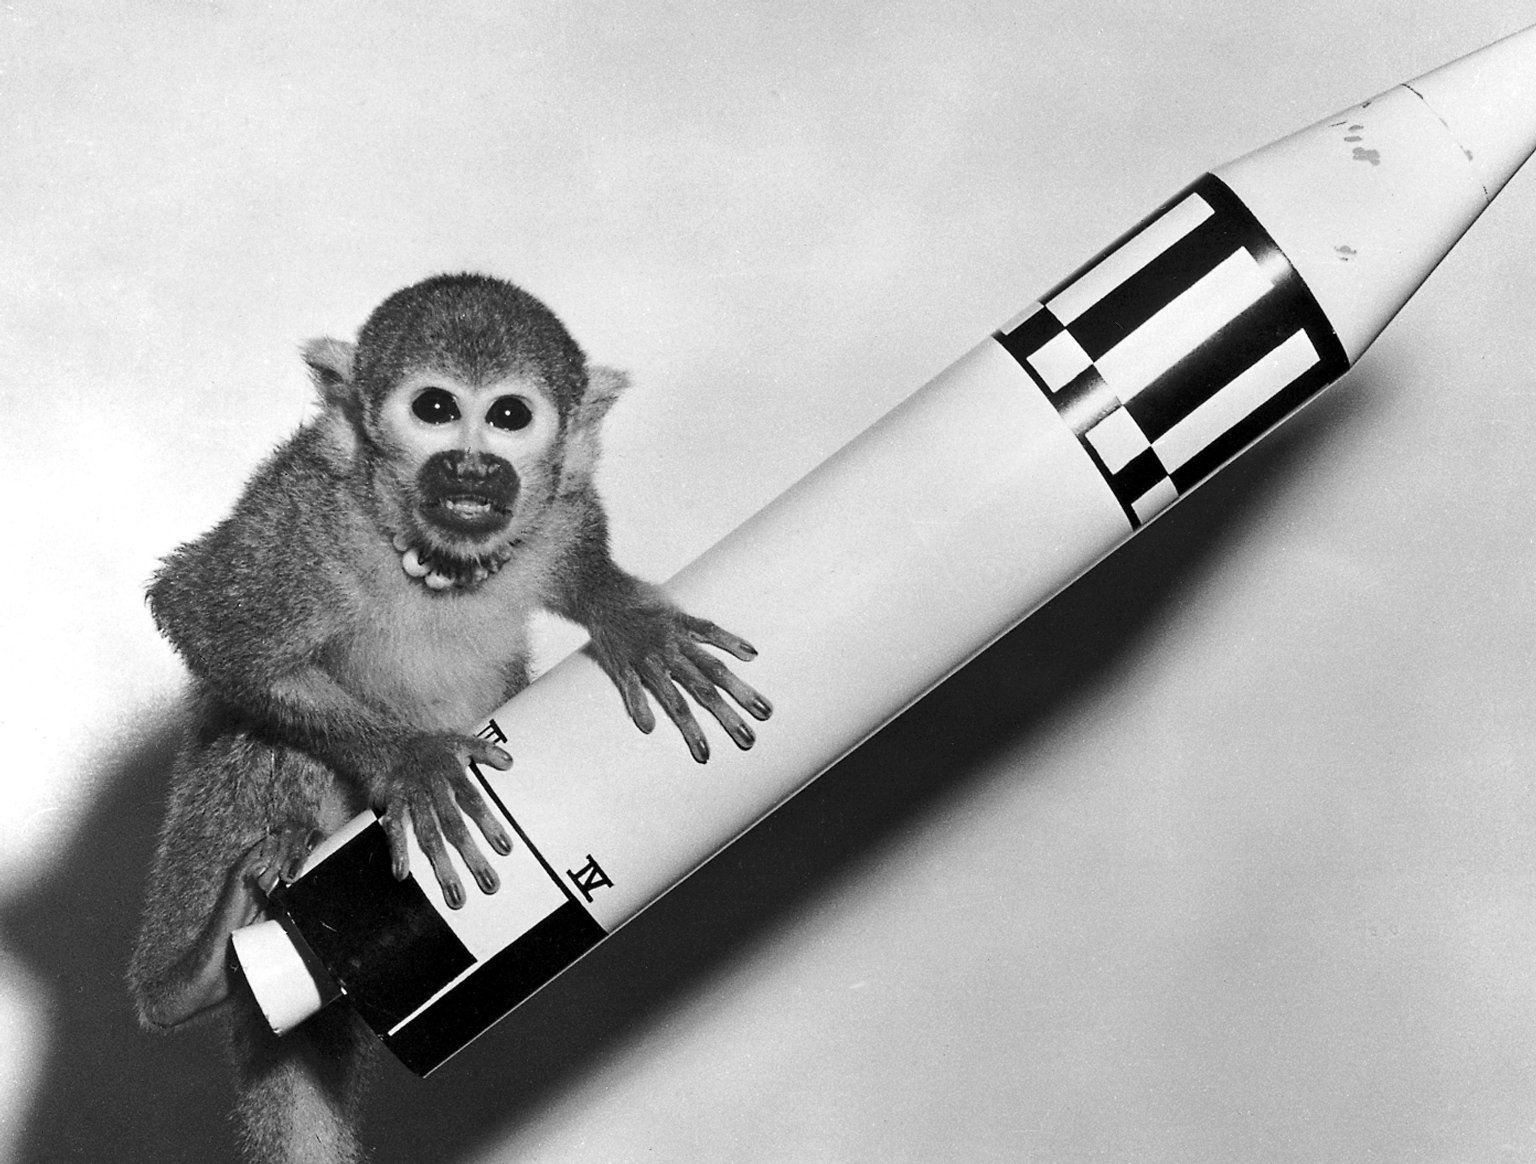
\includegraphics[width=.7\textwidth]{images/Baker}
%     \caption{Miss Baker was a squirrel monkey who went into space and back in 1959. This is her on a model of Jupiter AM-18, the rocket that took her into space.}
%     \label{image:missbaker}
% \end{figure}

% \clearpage
\subsection*{Respect the Laws of the Land}
Spirit Crossing, and Sneedville, are kind enough to be our home.  Here are some helpful tips on respect:
\begin{itemize}[noitemsep]
\item The property owner's house is off limits to participants.  Please be respectful of the land and grounds.
\item Although held on private property, TN Nudity Laws still apply. Please plan on wearing pasties, bikinis, loincloths, etc.
\item Please respect the land, the river, and the community.  Obey the speed limits and be courteous to those around you.
\item When in doubt, practice \textbf{consent}!
\item TTM  is an all ages event.  Those who are 21 or older will have a special wrist band indicating that they are able to legally consume alcohol. Please consume in moderation.
\end{itemize}
    
% \begin{multicols}{2}

% \subsection*{Alcohol}
% \gls{ttm} is an all ages event.  Those who are 21 or older will have a special wrist band indicating that they are able to legally consume alcohol.

% \subsection*{Camping}
% You may not camp in your car. Please bring a tent or RV / trailer.
% Cars may only be brought on site with approval.
% \bod[inline]{needs vetting}

% \subsection*{Code of Conduct}
% \Gls{ttm} now has a Code of Conduct. You can find it on page~\pageref{coc}.

\subsection*{Fireworks and Effects}
Fire effects with registered Theme Camps only, please.

\subsection*{\Gls{gifting}}\label{gifting}
This is a gifting community, providing refuge from everyday societal perils.  Once you're inside, no commercial activity takes place. Which is part of the charm, and the point :) 
Sometimes, there is a bit of a misconception of "Oh, so it's a barter system?" -- Actually, it's not. It's a "Gifting" Principle.
You gift without the expectation of a gift in return. 
You gift something to someone because at that moment, you feel the other person should have the very thing you'd like to give.

% \subsection*{\Gls{graywater}}
% There are no plans to dispose of gray water on site.  Each participant is responsible for \gls{pipo}.

% \subsection*{Nudity}
% TN Nudity Laws prohibit full or partial nudity on public property, and while we are on private property, the road cutting through Spirit Crossing is public, mostly accessed by residents, so very low traffic.

% We recommend you use discretion and wear pasties, paint, bikinis, etc.

\subsection*{Minors}
Minors must be accompanied by a parent or legal guardian. If they cause problems during the event which lead to possible safety issues or are a severe nuisance to others, we may ask you to remove the offending minor, possibly your entire camp. Minors are NOT allowed to use, play with, operate nor hold fire, fire props, fire effects and pyro, including poofers.  

%\subsection*{Public Health and Safety}

\subsection*{Recharging batteries for medical equipment}
Those with CPAPs and electronic scooters will have to make their own arrangements to recharge batteries.  \gls{ttm} does not provide battery recharging stations for medical equipment.

Some theme camps have generators, and may allow use of a spare generator plug for recharging medical equipment as a way of \gls{gifting}.  Home Depot and other companies also rent generators.  Moreover, there exist solar panels for recharging CPAP machines, though those can be prohibitively expensive.

\subsection*{Photography}
Please respect the right of others who may not wish to be photographed. Ask \textbf{permission}! If you see someone with a \textcolor{blue}{blue} wristband, that is a \textbf{no photo} policy indicator. 
Do not take pictures or video of participants wearing them! 

\subsection*{Sound}
To make this event enjoyable for all, amplified sound is limited to 300 Watts producing 90 db at 20 feet. All amplified sound is to be reduced after 4\am nightly to allow room for acoustic and ambient sound and to limit the possibility of neighboring sound complaints. 

\subsection*{Wristbands}
\label{sub:wristbands}
You will receive a wristband when you arrive at the \gls{gate}.  Different colored wristbands will identify you as being over 21, under 18, etc.  Wristband colors also indicate if you don't want your photo taken.  

You must keep your wristband on at all times.  See the \gls{gate} if you need to replace your wristband.

\subsection*{Vending}
No vending, selling, or promoting is allowed at the event.


\section*{Community Standards}

\subsection*{The Ten Principles}\label{tenprinciples}
Table \ref{tbl:tenprincples} on page \pageref{tbl:tenprincples} enumerates the 10 Principles of \gls{ttm}.
Funny thing about those: they are not meant to be chosen at random to suit ones need, mood or agenda, but according to our interpretation were created to work together as a whole.  
Meaning your right to radically and freely express yourself ends when your expression infringes upon another participant to do the same. 
In other words, they're not a "Getting out of jail free" card, nor a permission slip to be a dick. So don't be a dick, hiding behind one or two principles. 


\ifisflight
\begin{table*}[!ht]
\small
\centering
\caption[The 10 Principles]{The 10 Principles}
\label{tbl:tenprincples}
\begin{tabular}{@{}llp{2.9in}@{}}
\toprule
\textbf{No.} & \textbf{Principle}               & \textbf{Description}                                 \\ \midrule
1   & Radical Inclusion       & Everyone is welcome, all types, all kinds, friends, strangers, and in between.         \\[1em]
2   & Gifting                 & Gifts are unconditional offerings, whether material, service oriented, or even less tangible. Gifting does not ask for a return or an exchange for something else.        \\[1em]
3   & Decommodification       & Hand in hand with gifting, burns are environments with no commercial transactions or advertising. Nothing is for sale - we participate rather than consume.        \\[1em]
4   & Radical Self-Reliance   & You are responsible for you. Bring everything with you that you need. Burns are an opportunity for you to enjoy relying on yourself.          \\[1em]
5   & Radical Self-Expression & What are your gifts, talents, and joys? Only you can determine the form of your expression.         \\[1em]
6   & Communal Effort         & Cooperation and collaboration are cornerstones of the burn experience. We cooperate to build social networks, group spaces, and elaborate art, and we work together to support our creations.         \\[1em]
7   & Civic Responsibility    & Civic responsibility involves the agreements that provide for the public welfare and serve to keep society civil. Event organizers take responsibility for communicating these agreements to participants and conducting events in accordance with applicable laws.         \\[1em]
8   & Leaving No Trace        & In an effort to respect the environments where we hold our burns, we commit to leaving no trace of our events after we leave. This means everything that you bring with you goes home with you. Everyone cleans up after themselves, and whenever possible, we leave our hosting places better than we found them.            \\[1em]
9   & Participation           & The radical participation ethic means you are the event. Everyone works; everyone plays. No one is a spectator or consumer.        \\[1em]
10  & Immediacy               & From the Burning Man website : "Immediate experience is, in many ways, the most important touchstone of value in our culture. We seek to overcome barriers that stand between us and a recognition of our inner selves, the reality of those around us, participation in society, and contact with a natural world exceeding human powers. No idea can substitute for this experience."             \\ \bottomrule
\end{tabular}
\end{table*}
\else
\begin{table*}[h!]
\centering
\caption[The 10 Principles]{The 10 Principles}
\label{tbl:tenprincples}
\begin{tabular}{@{}llp{4.3in}@{}}
\toprule
\textbf{No.} & \textbf{Principle}               & \textbf{Description}                                 \\ \midrule
1   & Radical Inclusion       & Everyone is welcome, all types, all kinds, friends, strangers, and in between.         \\[1em]
2   & Gifting                 & Gifts are unconditional offerings, whether material, service oriented, or even less tangible. Gifting does not ask for a return or an exchange for something else.        \\[1em]
3   & Decommodification       & Hand in hand with gifting, burns are environments with no commercial transactions or advertising. Nothing is for sale - we participate rather than consume.        \\[1em]
4   & Radical Self-Reliance   & You are responsible for you. Bring everything with you that you need. Burns are an opportunity for you to enjoy relying on yourself.          \\[1em]
5   & Radical Self-Expression & What are your gifts, talents, and joys? Only you can determine the form of your expression.         \\[1em]
6   & Communal Effort         & Cooperation and collaboration are cornerstones of the burn experience. We cooperate to build social networks, group spaces, and elaborate art, and we work together to support our creations.         \\[1em]
7   & Civic Responsibility    & Civic responsibility involves the agreements that provide for the public welfare and serve to keep society civil. Event organizers take responsibility for communicating these agreements to participants and conducting events in accordance with applicable laws.         \\[1em]
8   & Leaving No Trace        & In an effort to respect the environments where we hold our burns, we commit to leaving no trace of our events after we leave. This means everything that you bring with you goes home with you. Everyone cleans up after themselves, and whenever possible, we leave our hosting places better than we found them.            \\[1em]
9   & Participation           & The radical participation ethic means you are the event. Everyone works; everyone plays. No one is a spectator or consumer.        \\[1em]
10  & Immediacy               & From the Burning Man website : "Immediate experience is, in many ways, the most important touchstone of value in our culture. We seek to overcome barriers that stand between us and a recognition of our inner selves, the reality of those around us, participation in society, and contact with a natural world exceeding human powers. No idea can substitute for this experience."             \\ \bottomrule
\end{tabular}
\end{table*}
\fi


% \clearpage
\subsection*{The 11th Principle -- Consent}

\gls{ttm} has adopted the 11th Principle, Consent\footnote{\url{http://www.11thprincipleconsent.org/2015/10/20/what-do-you-consent-to/}}.

% \begin{itemize}
\begin{labeling}{Photography:}
	\item[Touch:] Just because you hugged someone yesterday doesn't mean you can surprise them with a hug today. ``Surprise contact'' isn't always wanted, even if it's affectionate.
	\item[Foods:] Disclose the ingredients, one person's innocuous ingredient can be someone else's allergy.
	\item[Kink:] Consent for one thing isn't consent for another. If I said you can spank me, that doesn't give you permission to grope me.
	\item[Sex:] Consent can be revoked once it's been given.
	\item[Gifts:] Disclose what is in your gifts, even if it's just essential oils. Some people have sensitivities.
	\item[Photography:] Ask before taking pictures. Remember consent to take a picture is NOT consent to post it on your blog.
\end{labeling}
% \end{itemize}


\section*{Code of Conduct}
\label{coc}
TouchBass LLC / To The Moon Code are introducing a new Code of Conduct for 2018 and beyond.
If you are unable to agree to these terms and our policies, we’ll gladly issue a refund for your ticket.
Please contact us at connect@tothemoonburn.com. 

% \subsection*{The Moon Code Of Conduct}

% \begin{multicols}{2}
To The Moon, produced by TouchBass LLC, relies on attendees and volunteers to create and maintain a space that is welcoming for all ticketed participants. We don’t discriminate on gender, sexual orientation, disability, ethnicity, socioeconomic status, age, or religion and we abide by the Burning Man 10 Principles.

Participation in this event is open to all ticketed attendees, but is a privilege nonetheless. Attending privileges of To The Moon and related events sponsored by TouchBass LLC will be revoked if a participant fails to respect other attendees or behaves in a way that endangers themselves, the event, or the broader community as a whole.
Damaging behavior is not limited to violence or consent violations, but rather includes ALL behavior detrimental to The Moon as a whole, the burn itself, affiliated events, TouchBass LLC, its BOD, Team Leads, and volunteers and other participants by means of any actions in direct contradiction to and out of alignment with our mission:

\emph{“To The Moon exists solely to create a platform allowing its participants to unfold their creative wings and embrace and nurture a community striving to share their passions, unique gifts and talents and come together in celebration to do just that.”}

We want to impose upon your freedoms within our chosen community as little as possible, but need to protect our members and event at the same time.
The following are our policies designed to do just that.
If you experienced anything in violation of these guidelines, please fill out our incident report form to help us investigate.

Please note: 3rd Party Incident Reports are not accepted. The report has to be submitted by the person directly involved in / with the incident. If you feel the need to report something as a 3rd Party, please email us at connect@tothemoonburn.com.

\subsection*{Expected behavior includes, but is not limited to}

% \begin{itemize}[noitemsep]
	\subsubsection*{Consent}
    \begin{itemize}[noitemsep]
    	\item Obtaining someone’s consent in a sexual context is absolutely mandatory
        \item Obtaining consent for video or photography of a participant, or in any other way which potentially affects the experience of another person on The Moon is mandatory
	\end{itemize}
        
    \subsubsection*{Non Consensual}
    \begin{itemize}[noitemsep]
        \item Be considerate and respectful of fellow participants and the community around the event.
        \item Refrain from non-consensual demeaning, discriminatory, or harassing behavior.
        \item Be mindful of your surroundings and of your fellow participants’ safety.
	\end{itemize}
% \end{itemize}

\subsection*{Unacceptable behavior includes but is not limited to}
\begin{itemize}[noitemsep]
    \item Predatory behavior, defined as any unwanted and non-consensual form of the following
    \begin{itemize}[noitemsep]
        \item Non-consensual physical contact, including unwelcome sexual interaction
        \item Intimidation, harassment, stalking
        \item Verbal or physical abuse
        \item Spousal abuse
        \item Violence against other participants or their property.
	\end{itemize}
         
    \item Abuse or neglect of To The Moon or land owner’s property, physical or otherwise, such as vandalism, theft of event property
     
    \item Sabotaging To The Moon, its Event Leads and other TouchBass LLC sponsored events, and the BOD by (including but not limited to)
    \begin{itemize}[noitemsep]
        \item Willfully perpetuating false information about TouchBass LLC’s operating procedure
        \item Intentionally damaging relationships fostered by To The Moon for future events by exhibiting aggressive or manipulative behaviors toward hosts and attendees of Touch Bass LLC events
        \item Deliberately harassing BOD members, Team Leads, volunteers or participants for the sole purpose of undermining TouchBass LLC Leadership, its BOD,  operating procedure, events and mission.  
	\end{itemize}

	\item Disrespecting the local community around the event by
    \begin{itemize}[noitemsep]
        \item Dumping trash in local dumpsters
        \item Trespassing
        \item Repeated violations of the event’s sound ordinance
    \end{itemize}

	\item Disregard for one’s own safety (including intentional self harm or intention of) or well-being to such an extent it demands the intervention of other participants, community members, Team and / or Event Leads. volunteers or outside agencies, such as intervention by local law enforcement or fire department staff.
    
	\item Repeated or egregious violations of any and all policies put in effect by event organizers.
    
    \item Defiance against Rangers or other Safety Team Leads, Event Leads and land owner handling a potentially dangerous or life threatening situation.
    
    \item Breaching Perimeter at any effigy / temple burn
\end{itemize}

\subsection*{Consequences of unacceptable behavior}
Unacceptable behavior will not be tolerated. This includes additional forms of said behavior at the burn as well as pre- or post-burn events and via all forms of communication across all platforms.

\textbf{Anyone asked to stop unacceptable behavior is expected to comply immediately.}

Participants who engage in unacceptable behaviors will be subject to event organizers action deemed appropriate to ensure the safety of the event, its affiliate events and affiliate relationships and its participants.
This action may include expulsion from the event without refund, revoking tickets, removing a volunteer from their shift, and temporary or permanent bans from TouchBass LLC events.
\ifisflight
\newpage
\fi
If a participant’s behavior does not comply with this code of conduct, does not align with our mission, or puts the future of TouchBass events at risk, (i.e. our burn, Town Halls, Fundraisers) a suspension for the present or following years may be imposed.
Suspensions may not be permanent, and appeals may be submitted in writing in cases where conflict resolution is demonstrated by the offending party. The appeal’s timeline is determined by TouchBass LLc and will be resolved between members of the Board and the suspended party.

TouchBass LLC or individuals may pursue potential legal action.

\ifisflight
\vspace*{\fill}
\begin{figure}[!h]
\centering
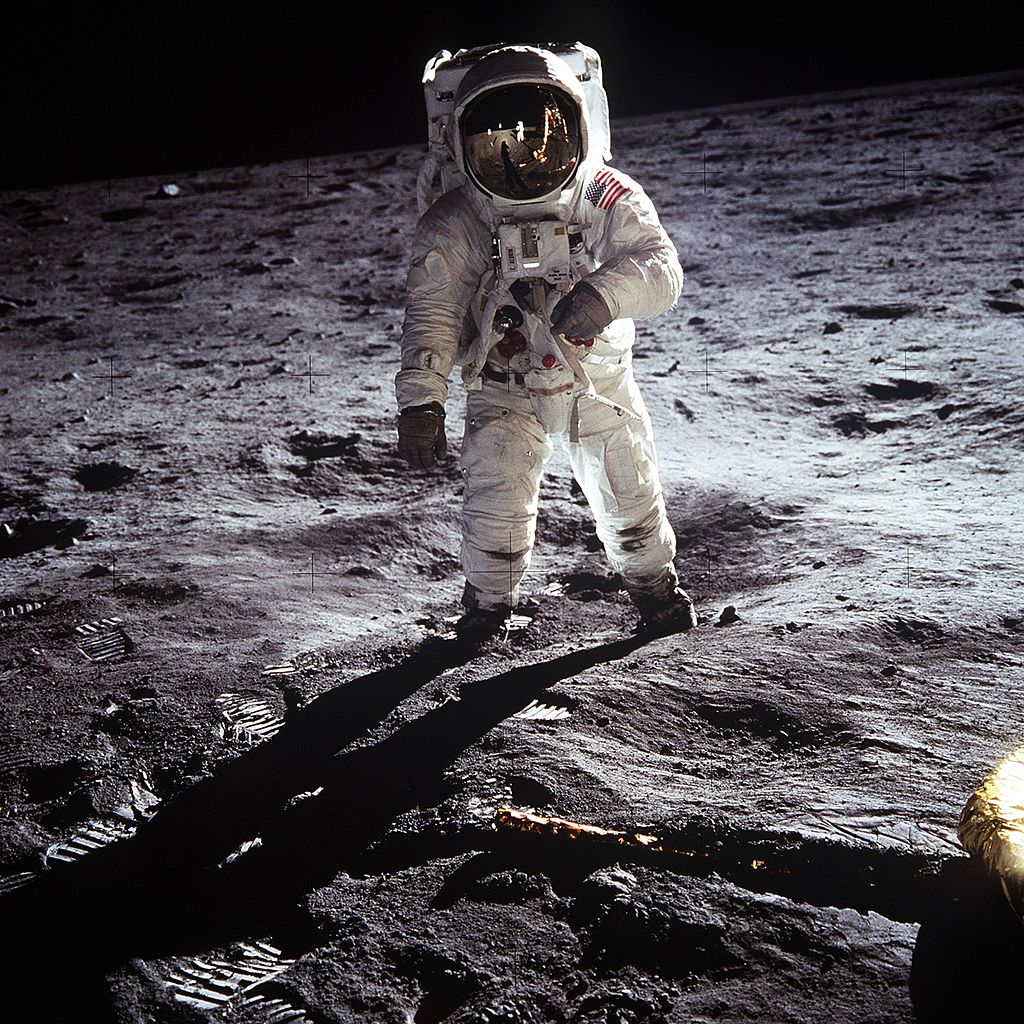
\includegraphics[width=\textwidth, trim=65 0 55 0, clip]{images/Aldrin_Apollo_11.jpg}
\caption{Cool astronauts follow the rules while they frolick on the moon.}
\label{image:firststep}
\end{figure}
\vspace*{\fill}

\fi
% \begin{table*}[!ht]
\small
\centering
\caption[The 10 Principles]{The 10 Principles}
\label{tbl:tenprincples}
\begin{tabular}{@{}llp{2.9in}@{}}
\toprule
\textbf{No.} & \textbf{Principle}               & \textbf{Description}                                 \\ \midrule
1   & Radical Inclusion       & Everyone is welcome, all types, all kinds, friends, strangers, and in between.         \\[1em]
2   & Gifting                 & Gifts are unconditional offerings, whether material, service oriented, or even less tangible. Gifting does not ask for a return or an exchange for something else.        \\[1em]
3   & Decommodification       & Hand in hand with gifting, burns are environments with no commercial transactions or advertising. Nothing is for sale - we participate rather than consume.        \\[1em]
4   & Radical Self-Reliance   & You are responsible for you. Bring everything with you that you need. Burns are an opportunity for you to enjoy relying on yourself.          \\[1em]
5   & Radical Self-Expression & What are your gifts, talents, and joys? Only you can determine the form of your expression.         \\[1em]
6   & Communal Effort         & Cooperation and collaboration are cornerstones of the burn experience. We cooperate to build social networks, group spaces, and elaborate art, and we work together to support our creations.         \\[1em]
7   & Civic Responsibility    & Civic responsibility involves the agreements that provide for the public welfare and serve to keep society civil. Event organizers take responsibility for communicating these agreements to participants and conducting events in accordance with applicable laws.         \\[1em]
8   & Leaving No Trace        & In an effort to respect the environments where we hold our burns, we commit to leaving no trace of our events after we leave. This means everything that you bring with you goes home with you. Everyone cleans up after themselves, and whenever possible, we leave our hosting places better than we found them.            \\[1em]
9   & Participation           & The radical participation ethic means you are the event. Everyone works; everyone plays. No one is a spectator or consumer.        \\[1em]
10  & Immediacy               & From the Burning Man website : "Immediate experience is, in many ways, the most important touchstone of value in our culture. We seek to overcome barriers that stand between us and a recognition of our inner selves, the reality of those around us, participation in society, and contact with a natural world exceeding human powers. No idea can substitute for this experience."             \\ \bottomrule
\end{tabular}
\end{table*}
% \input{astrotraining2}

% how we can each contribute to the burn
%
% Here are the many ways folks can help out.
%
% TODO I know I'm missing lots.  :-\
%

\chapter{Volunteering}

No burn exists without volunteers and volunteers are our heroes! We have no hired help other than security and everything we do is done on a volunteer basis.  This goes for all the things before, during, and after the burn.  All the teams that you can volunteer for are described in the ``Crew Manifest'' section starting from page \pageref{ch:teams}.

There are two ways to volunteer:

\textbf{Before the event} you can sign up from the available volunteer activities by going to:

{\indent ~~~ \url{https://www.signupgenius.com/tabs/33773df01a4c3edc42-tothemoon} }

\textbf{During the event} you can go to the \gls{vc} folks at the \gls{cockpit} to sign up for an available volunteer slot.

\section*{EARLY ENTRY FOR VOLUNTEERS}

If a participant has a volunteer shift on Wednesday, they will be granted entry at noon on Wednesday. \footnote{This is mainly \gls{gate} but a few other teams have a few volunteer shift scheduled for Wednesday for set up.}  If a participant has a volunteer shift beginning before noon on Thursday they will be granted early entry on Wednesday after 3 pm.  This list will be given to \gls{gate} from \gls{vc} before \gls{gate} opens opens on Wednesday.

All participants must be off site by noon on Monday unless they have a shift on Monday after noon. In which case they will need to have permission from \gls{vc} or one of the \gls{eventleads} to stay on site for that shift, and should stop by the \gls{vc} tent on Monday before 10 am to get their approval. All late stay volunteer must also have their camp packed before their shift on Monday and be prepared to leave immediately following that last shift.\footnote{There are other early entries granted for \glspl{themecamp}, \gls{dpw}, \glspl{teamleads}, \gls{bod}, etc,,  but those lists will be given to \gls{gate} from appropriate lead for that team. This info is just for those volunteering first shifts on teams that start when gates open or before.}


\clearpage
\section*{Volunteer Training}

\subsection*{Conclave}
We ask that all fire spinners attend one of the the three fire safety meetings provided by Singe City and obtain a wristband. This will allow you to come spin in their fire circle each night in Headroom Village. 

Fire safety meeting will be at Singe City fire circle in Headroom Village:
Spinners in conclave must attend one of the training events listed below.
You will be given a fire safe wristband to spin fire during the burn. Conclave participants should meet at \gls{effigyburnfield} at 3:00\pm{} Saturday evening.

\begin{center}
\begin{tabular}{|c|c|c|}
\hline
\textbf{Day} & \textbf{Time} & \textbf{Place} \\ \hline
Thursday & 5\pm{} & Singe City fire circle in Headroom Village \\ \hline
Friday & 5\pm{} & Singe City fire circle in Headroom Village  \\ \hline
Saturday & 5\pm{} & Singe City fire circle in Headroom Village  \\ \hline
\end{tabular}
\end{center}

% \clearpage

\subsection*{Perimeter}
Outer Perimeter volunteers meet at the \gls{effigyburnfield} on before the burn at the times listed below for training/instructions. Friday and Sunday for the two temple burns, volunteers will stay at the \gls{effigyburnfield} until the burn. Saturday, the training is well before the burn. Volunteers will be given a break, and meet again at the specific time given at training.

If you are experienced with perimeter and fire safety and want a shift doing \textbf{inner} perimeter, please email the perimeter lead directly (\url{perimeter@tothemoonburn.com}) and they will vet you for that.

\begin{center}
\begin{tabular}{|c|c|c|}
\hline
\textbf{Day} & \textbf{Time} & \textbf{Place} \\ \hline
Friday & 8:15\pm{} & \gls{effigyburnfield} \\ \hline
Saturday & 4\pm{} & \gls{effigyburnfield} \\ \hline
Sunday & 6:30\pm{} & \gls{effigyburnfield} \\ \hline
\end{tabular}
\end{center}


\subsection*{Rangers and Fire Safety}

\begin{center}
\begin{tabular}{|c|c|c|}
\hline
\textbf{Day} & \textbf{Time} & \textbf{Place} \\ \hline
Thursday & 7\pm{} & \gls{moonrangerstation} \\ \hline
Friday & 1\pm{} & \gls{moonrangerstation} \\ \hline
Saturday & 1\pm{} & \gls{moonrangerstation} \\ \hline
\end{tabular}
\end{center}

\subsection*{River Safety}

Note that this safety training is open to everyone.  Anyone that wants to play in the river is strongly encouraged to attend.

\begin{center}
\begin{tabular}{|c|c|c|}
\hline
\textbf{Day} & \textbf{Time} & \textbf{Place} \\ \hline
Friday & 1:30\pm{} & Riverfront below \gls{dpw} \\ \hline
\end{tabular}
\end{center}

\vbox{
\subsection*{Tbase / Sanctuary}
You will also be able to sign up for volunteer shifts at the burn, at the end of the training, or you may sign up for shifts now as long as you attend a training before your shift is scheduled.

\begin{center}
\begin{tabular}{|c|c|c|}
\hline
\textbf{Day} & \textbf{Time} & \textbf{Place} \\ \hline
Thursday & 6\pm{} & \gls{tbass} \\ \hline
Friday & 7\pm{} & \gls{tbass} \\ \hline
\end{tabular}
\end{center}}

% \bod[inline]{add all volunteer training}
% \todo[inline]{Add information on how to volunteer before and during the event. Probably from https://www.tothemoonburn.com/volunteering}
\vfill
\begin{figure}[H]
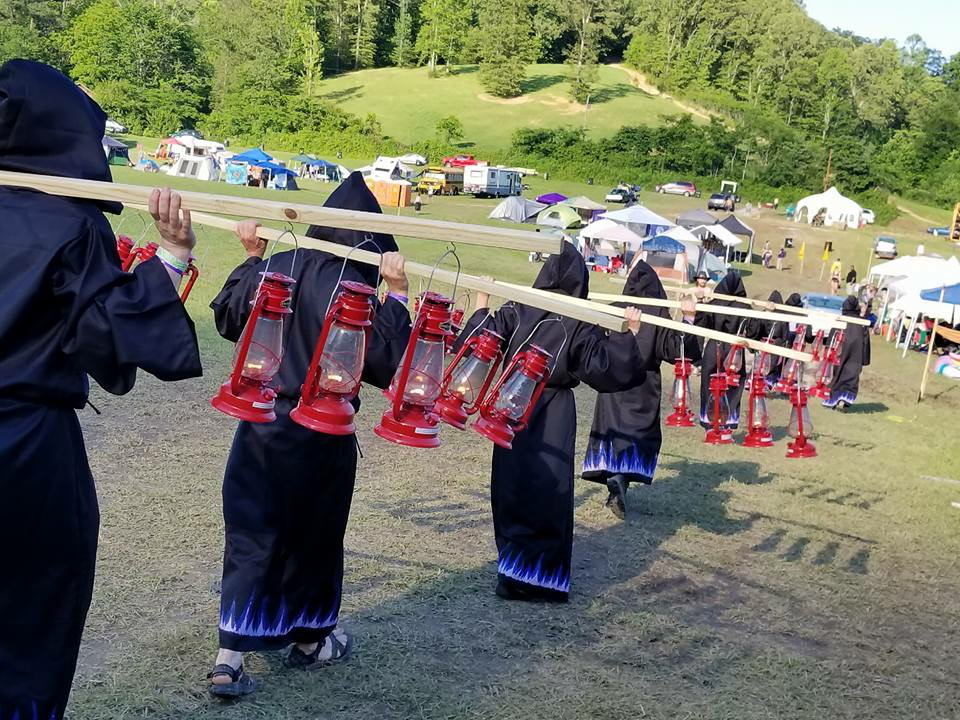
\includegraphics[width=\textwidth]{images/lamplighters.jpeg}
\caption{Lamplighters at work. Image courtesy of Johnny “Twaffle” Benton, 2017.}
\label{fig:lamplighters2017}
\end{figure}


% part of the reason why we're here, yes?  :)
%
% Part of the reason why we go to burns, AMIRIGHT?
%

\chapter{Art}


\begin{multicols}{2}


\section*{Funded Art}

\subsection*{3rdeyeluminart by Loren shaw}
        Live painting

\subsection*{Adrift' Shuttle by Johnie "Five" Waddell}
         Transporting people to the drop off point for floating the river by day and will be         an amazing LED art car by night: makes for a great companion to any stage.        


\subsection*{Appalachian Art Lab by Stacy Kraft / Running Doe                       }
Hi! Running Doe here! Come experience the element of neon visually represented through a series of black-light reflective abstract art. We are bringing back the Make-Your-Own-Dream flags for the Temple Burn and will have a table set up with fabric and markers for you to come and create as you please throughout the weekend. Depending on the weather and humidity, we might do an art demo on Friday. Much love, Running Doe


\subsection*{Art Carts What What! by Alannah "sole" Tomich        }
Have you arrived on the moon and want to start enjoying burny art projects but still have to unload and build your camp? Have a lot to haul to get your camp packed-up but your car might get stuck in the mud? The Acrodesiac Lunartics (AcroYoga camp) presents ArtCarts, decorated mobile art pieces for all your camp gear transport needs with heavy duty wheels for the mud. To help you arrive on the moon with ease and color and burner spirit. Come check out our elemental designs. Let’s be gentle on the meadow (leave no trace) and come borrow an ArtCart from our stand. 


\subsection*{BLAST OFF by Caitlin and Sassy Noodle                }
Ooooo we flying in the spaceship, back to the basics, back to the matrix. Strictly constructed of cardboard and awesomeness. Crawl in through the space hole and be blasted off into another dimension. My spaceship is equipped with comfy, cushy, pillows to sit and relax and gander up at the nicely painted glow in the dark stars that’ll make you feel as if space really is surrounding you. Feel the interstellar vibes from the ambient music that will be playing throughout the night when the sun goes down and the moon comes out. Come BLAST OFF.        
                
\subsection*{The Bizarre Bazaar        by Robert Blew        }
"A theme camp featuring a 20 ft tall teepee in the center that provides a cozy space for wandering burners to take respite from the stress of the burn and smoke hookah in a comfortable lounge. Nearby, they can enjoy the booths that make the "Bazaar" part of our camp, including our "secret shop" for undisclosed curiosities, art booth for the viewing of camp-member-made trippy art, a distillery for a sampling of flavored moonshines made by camp members, and an artisanal coffee bar for a selection of espressos, cold brews, lattes, and the like.


\subsection*{The Blue Box by Jessica Logan                 }
        A full scale replica of the Doctor Who TARDIS.


\subsection*{The Booth Fairy by Elle Erickson                }
        Super fantastic and interactive Free advice booth




\subsection*{Booty Prints by Ashley Humphries                        }
Booty beautification imprintation is being brilliantly brought to you by Ashley the asscommander of Alcoholic Alliterators. Stop by our booty beautification booth to have your booty beautified and then captured creatively on a flat medium to take home with you. The booth will be open at choice times to accommodate your accentuated assets. So come by, grab an alcoholic alliteration and print your posterior.


\subsection*{The Brownie Brothel by Catherine Nguyen (no burner name... yet)        }
The Brownie Brothel is the leading purveyor of from-scratch, gourmet, artisan desserts to the Georgia Burns, and we're excited to bring our sweets to To The Moon for the first time. As done for past events, we plan to bake and distribute a wide variety of tasty, ranger-safe baked goods to all and sundry, including those with dietary restrictions. In addition, our goal is to use baked goods to teach the community lessons about engaging in healthy consent habits.


\subsection*{Clean Hippies Taste Better         by Erick Bixler/ MavErick Cadabra         }
Come wash away your woes at camp “clean hippies taste better”. We will be providing 2 hot/cold water showers, hot/cold pools, and a chill dry space to change and regroup before you blast off around the moon again. Join us Friday night and sat night at 1am and again Sunday at 10\pm for our shower disco party. All the steamy showers in one big room for 2 sweet hours. Get clean or get weird. Just clean up the mashed potatoes when you’re done.         


\subsection*{Clouds on the Moon by Dorne Pentes/ Awesome                }
A small, experiential moon-like space consisting of LED clouds moving and changing to music. Housed in a small geodesic dome with pillows and blankies to lie on and watch it move.


\subsection*{Connecting Through Eye Contact by Ashley Maynard (Bones)                }
Hang out with a stranger, or a friend, and maintain eye contact for 1 minute.  Feel their spirit within you and share your spirit with them.  Re-establish the human experience and enter the windows to the soul.         

\subsection*{Countdown by Aaron Averill}

Enter the capsule. Experience the universe falling away as you are bathed in rhythmic changing lights. Meditate and look inward, or enjoy with a friend or two.


\subsection*{Cosmic Express by Willow Gaia and Kris Totillo}
Float along with the GOATs! Ride on the majestic cosmic farty cloud. Greatest of all Time; Moon tours and exhibitionists daily!


\subsection*{Cutie Clinic by EVP Grace Tsaritsa                        }
Oooo pretty pastel colors! But wait...this is kinda creepy. That's the whole point of our happy hospital, taking uncomfortable topics like chronic and mental illness and making them refreshingly kawaii. This interactive installation is based around the Japanese street style Menhera, also known as yumekawaii or "sick cute".We invite you to look at our magical pieces, make your own get well soon cards, or hang out in our cuddly stuffie pool. Remember: your health should be your first priority!


\subsection*{Dancing Fungi by Jeremy Bourque                }
An interactive art camp/mushroom fairy garden consisting of a large mushroom cottage made entirely out of recycled materials, with a repurposed satellite dish for a roof, a light up mushroom garden, mushroom art, a creation station for attendants to make their own arts and crafts, and speakers and lights throughout. The cottage will have various features, such as a dj booth, dance floor and a stripper pole, and lots of hidden surprises.


\subsection*{Dream Scarf by Nicole Sholtis                 }
I'll be wearing a special scarf made of small pieces of paper and safety pins. All you have to do is write down a hope, a dream, a goal, a wish... roll the paper up and pin it to the scarf that will burn with effigy.        


\subsection*{Dream Weaver Manifestation Station by Holly Hamel - Mother Superior        }
"We all have our own life to pursue, our own kind of dream to be weaving, and we all have the power to make wishes come true, as long as we keep believing."   -- Louisa May Alcott      
The Dreamweaver Manifestation Station is a giant dreamcatcher interactive art piece that works through the Law of Attraction. You, the Dreamer, are offered an opportunity make an intentional wish for your heart’s truest desire. The Intender’s Circle will add our powers of manifestation to your dream, with the caveat that all is in the best interest for YOU and your journey. Be sure to send feedback of your manifestations coming true to holly.mothersuperior@gmail.com!


\subsection*{Element Altar and Affirmation Station by Rachael Peak                 }
A peaceful small place with an altar to the elements in the same space is an affirmation station. Words are powerful. Hundreds of artsy and laminated positive quotes, mantras and affirmations will be in a big treasure chest for burners to look at, or to take one to help then with their day/life. Also, there will be a creative spot to write down manifestations that will likely be burned at the end.


\subsection*{Elemental Pillars        by Andrea Long (Andi Glytch)        }
The EleMENTAL pillars will tower above and look over us all, turning nature into interactive visual art! Our four elemental symbols will stand tall for most of our journey and eventually burn with the fire of the gods!        


\subsection*{ElemenTapestries by Aaron Robbins                }
Tapestries made out of old sheets from thrift stores. We use a technique that we call faux batik. We use washable glue to create an image then paint it with acrylics. The fabric is then washed out, so that anywhere there was glue remains white. The resulting image looks like batik, tie dye and stained glass.


\subsection*{Envision by Sidhe •. Natalie Starr Mudd                }
A Temporary Kinetic Sculpture and Sacred Space made of thousands of holographic palettes. These cascading holographic shapes dance and sparkle in the breeze, creating a mesmerizing iridescent shimmer, similar to light reflecting off rippling water, or sunlight dappling through the leaves. Come and sit a spell. <3        


\subsection*{Eons of Neon: The Fluoresciverse by Tyler Key, TzKey ( Beast)                 }
A giant, 360 degree, neon, fluorescent, black-light-reactive mural. Imagine standing in a circular room, the sky is your ceiling, the walls are 8 feet tall with mesh screening, covered in murals, bathed in black light, and in the middle of the room are blankets, pillows, inflatable couches and chairs, and bean bags.


\subsection*{The Euphoria Temple by Patrick Murphy        }
        We built the temple for Euphoria, but unfortunately Euphoria didn't happen :( We         want to share our temple with burners, and hope to be able to burn it at To The         Moon.        


\subsection*{Feathered Ear Cuff Crafting Workshop by Pralla de la Torre aka Le Klo                }
Come see us Friday and Saturday to make some killer accessories over at Memento Trio! Bring feathers, beads, or wire if you want! We are gonna craft it upppp! Special thanks to Victoria for helping me hash out the details on this process!


\subsection*{Flower Crown Workshop by Bethany Stonestreet - Mother Superior        }
        Make your own flower crown from fresh, real flowers. Saturday from noon-2p.


\subsection*{Fly me to the Moon }
        A large aerial rig decorated with lights.        


\subsection*{Forever Flowers by Holly Ross                   }
"Forever Flowers” is a beautiful recycling effort that started out as a simple yard art project.   The flowers are made of metal cans, plastic water bottles, lids, etc, and are then painted with bright colors.  This cheery installation aims to bring awareness to the importance of recycling - each flower is a visual representation of a piece of “trash” that will not end up in a landfill or the ocean.  The collection also serves as a haunting reminder of how much trash we create individually. I hope to inspire others to view one-time use packaging as valuable material that can (and should be) reused in creative ways! 


\subsection*{Fricken Laser Beams by Larry Kresse        }
Beams of light that will scan across the tree line at a speed such that humans only see pulsating planes of multicolored light, extending into the horizon.         


\subsection*{Genizm's Manifestation of Light by Genizm (Gurudev and Klay.Ra)                }
"Hello! Here's a quick bit about our art:


   * – GxR's The Manifestation of Light – *
             fri and sat after dark


-> electro jamz by Genizm + vocal improv by Klay.Ra |
-> co-creative audiovisual experience with LaZeRs   | 
-> we invite you to come jam, boogie, or just be    


\subsection*{Heart Melt Café by Katie Gentner "Kitty"                 }
Share a sweet and refreshing ice cream sundae with a new person! To participate take a number and wait to be served! Feel free to join the audience and witness all of the heart melting moments! 


Open Daily: 1-2:30pm, and 7-8:30pm


(Lactose-free vegan ice cream available upon request.)


\subsection*{Hey Y'all: Ain't Yo Mama's Front Porch by Lauren Yanochik and Blake Dunaway                }
The burner version of a good old fashioned front porch for your enjoyment. We will have a bar that serves all the sweet tea you could want and more, all the southern snacks we grew up on, and music of all genres from the great state of Georgia; we will even try to accommodate requests. We will have an illuminated marquee that will list our featured drinks and snacks daily. Come sit with us, either under the porch surrounded by flowers and candles, or by our fire, and share your best "southernisms" on our interactive art project which will consist of a free-standing three panel display blank map (because we also wanna know where y'all from). Sharing a little southern comfort is our goal, and we hope to see all y'all on the porch!


\subsection*{Jellyfish Umbrellas and Flying Squids!        by Elaine Pastor                }
We have electroluminescent jellyfish umbrellas for night use and we are purchasing large jellyfish kites to fly mid-day with a group squid/octopus/jellyfish field frolicking. The umbrellas will be available for others to use and return.        


\subsection*{Lumina by Katie Herman                }
Concentric circles of multi colored luminaries to create a peaceful, calm space for wandering and relaxation at night.


\subsection*{Mehndi Moon SPAce Station by Peaches (Dawn Strickland) and Emi Piez                        }
Divine Goddess Cosmonauts aiding you in your space travels sounds like a stellar dream… come let us make it come true at the Mehndi Moon SPAce Station. Passing astronauts will feel right at home in our antigravity chairs and chaise lounge as they breathe in the aromatic atmosphere within the SPAce Station. The Station will provide several amoonities while aiding those extraterrestrials bravely participating in the Dream Weaver Manifestation Station. Nebulax with our selection of essential oil mists and cooling sarongs. Have your celestial body decorated with henna designs and have your celestial toes painted with paint that glows. Feeling lost in space? We all are, but at Mehndi Moon SPAce Station we will jettison you into a new orbit of planetary pampering.


\subsection*{Memento Serenous        by Niklas "Unicrash" Gahm           }
A burn is a peak of Eristic Energies as we are swept up in the delightfully energetic cavalcade of art, with rare moments of self-preservation and calmness at the temple. But what if we could collectively generate a sound or collection of sounds that center us in the non-silence? SINGING BOWLS. SO MANY SINGING BOWLS. This is an installation entirely focused on the clarity and crispness of a sound delightful. We do not know where this sound may take us, but it can serve as a centering call to rally our spirits as we grow weary with exertion in the expanding exploration of a burn unknown.


\subsection*{The Oracle Is... by Ian Rhett                }
An unassuming "Charlie-Brown" desk with two attached chairs and a (solar-powered) illuminated sign that says "The Oracle Is..." and a flippable "In/Out" beneath it invites anyone to be the Oracle and to dispense Oracle-style futurisms. The desk will be moved throughout the event and will, at one point every day, be staffed by the artist, channeling The Oracle.


\subsection*{Paint by Burners by Olivia Holladay                }
Come paint on the canvases! Free range to paint whatever you want! Add to what other burners have started! Lay the foundation of the master piece that will be added to every burn!


\subsection*{Patchwork Tee Pees by Rachael Marshall                 }
I created Patchwork teepees to bring special energy to the space, experience special moments with the people around me, and to create space to open people up and be free to express themselves through the beauty of art. The traditional teepee was not only an efficient structure, but also a symbolic expression of humanity’s relations with the natural and spiritual worlds. Especially in the case of ceremonial teepees, the process of obtaining hides and poles was and is shaped by prayer and ritual guidelines. Symbols and story drawings were often painted on both the interior and exterior of the teepee, and these drawings were often the expression of visionary experiences. Like the Buddhist stupa or the Hindu mandir, the space created by the teepee is itself symbolic of the wider cosmos: time and the seasons, space and the four directions are associated with the circular floor space of the teepee. In its circle are structured many of life’s activities, from the most mundane to the most sacred. The circle of the teepee is a profound symbol of the interdependence of all of life. I have built the teepees for everyone to come and create space in and share with everyone else to collectively build energy that will grow and resonate through the burn.


\subsection*{Perception Pyramid        by Bryan Bell        }
"Oh, we flood your eyeballs, over, overload your, uh, your earballs, I give you patterns and swirls of color, and, uh, makin’ you feel better and better, yeah, the power of using light to, uh, to enhance consciousness and alter consciousness is the tricks I’m using now, and, so far, they’re legal." -Tim Leary                




\subsection*{Pop        by Kent Davis   }
        A place where volunteers can come get a little coffee have a bite to eat daily!         


\subsection*{The Pussy Palace        by Sara Wright / KC Lepp        }
We will be providing a Playful Kitty Fun-house for all ages. The structure will include:
- Rooms you can crawl through
- Giant oversized cat toys (ex: giant bubble wands, rubix cubes)
- Large slide designed as a cat tongue coming out of a cat head
- An infinity mirror room with furry walls
- Porch lounge area
- Color changing light features
- Rope net
- Covered cuddle puddle pit room
- Scratching and massage post




\subsection*{RV Life by Kimberly Lindemann/Jade                }
A newly remodeled motorhome “open house” where there will be tours and talk with burners about minimalism, downsizing, and how to get started. 


\subsection*{Space Dome        by Rania Glass / Scarlet        }
A temperature-regulated "chill space" for wayward action hippies to relax, make conversation, and cuddle with our assorted floofs under the watchful eye of the Octopoolpus.        


\subsection*{Sherpa Guided Meditation and art journey by Merri Benham         }
Art booth and night time guided meditation to inspire your evening's journey with awareness and love.


\subsection*{Star City by Trinity White and John LaCount (Sphinx and Teddy Bear)                Tree        }
An exploratory space within the trees made out of several tentsiles and sacred geometry hoop art.


\subsection*{Survival Guide by Piprrr, Raptor, and Bones}

You're looking at it.  ;)

The \gls{survivalguide} is not just intended to inform --- to give enough information for crew to plan and prepare as well as to navigate \gls{ttm} --- but is also our art contribution to the burn.  We hope you enjoy it as much as we enjoyed putting it together for all of you.



\subsection*{Swing, swang, sung by Evans Manrique                 }
        Swings for adults to feel like kids again.        




\subsection*{To The Moon Photo Booth by NativeEye Photography                 }
Dawn the neon! Jump in your space suit!
Grab your crew get ready for blast off >>>>>TO THE MOOOOOONNN!
You and your team are venturing to the moon to collect samples and protect each other inside my blacklight moon landing photo booth!
Grab your space team come on down to the burning yacht club camp! Grab some props and samples and jump in the booth for photo shoot fun. Bring a phone for me to snap so you can share with your crew!


\subsection*{Under the Stars by Gene                         }
Visual projectors of stars under our cool stretch tent. Come hang out at The Burning Yacht Club


\subsection*{Where my Beaches At?! by Aaron Shugart-Brown and Dorothy Verbick}
This interactive art installation is a beach style double seating chair elevated at about 12 ft off the ground, complete with plenty of amenities that will bring the attitude and playfulness of the beach TO THE MOON. Imagine yourself watching the “ocean” (river) of people mull about, throw down your rescue rope and make the buddy system come alive. Styling out under the umbrella our beach tower comes with all the fun in the sun that you would ever dream up! Complete with Zinc Oxide, Mounted Beach Umbrella, Hand Crank Weather Radio, Bulletin Board (missed connections, lost and found, general information), Megaphone, Life Preserver, Costume Chest, and Binoculars. Take notes on the clipboard, Spot a new friend, and throw the lifebuoy - we are proposing a fully immersive experience that promotes taking on the “responsibilities” of being a lifeguard at a burn. The 11 principles and a map will be posted on the structure. These stations can also be used by the Rangers for safety purposes if needed.                        


\subsection*{Yarn Doll Moon Spirits by Thomas O’Connor and Caleb Franklin                }
A cozy interactive art installation with a make-your-own yarn doll crafting station for others to take and leave dolls, make and gift yarn creations. There are plans for large rope scultptures imitating yarn dolls surrounding a large area with rugs, pillows, piles of yarn, string, safety scissors, beads, and charms to create. there will be walls where you can hang them, along with long may-pole like strings to clothespin dolls for gifting tree purposes.

\section*{Funded Burn Art}

\subsection*{Euphoria Temple by Patrick Murphy and Katie Herman}

Friday night Euphoria Temple Burn in dedication of Larry Harvey "The Man in the Hat".

This Temple was originally created for Euphoria this year.  When Euphoria was canceled, the stars aligned and it found its place at To The Moon.  It houses dozens of pieces of laser cut art created by the Georgia burn community, creating an engaging mix of light and shadow once the sun goes down.  

\subsection*{Sunday TTM Temple by  Michael "Lunar" Luber and Matthew Horner}
We would like to introduce the ElemenTemple! This is where Fire, Water, Earth and Air, join with the Spirit, brought together through an eclectic collaboration of art! This will be in the lower level. 
From the ground to the sky will be the connection of the creation, the universe and all, sending a beacon of light into the sky.
The ElemenTemple burn will be at dusk/dark:30 Sunday evening, so please plan on hanging out to send her to the skies and back.

Please feel free as always to write your dreams and wishes, anything you want to take in or let go of, and if you would like to keep them private, there will be paper to write on that will remain confidential, that I will hang in the temple before we send it up.
See ya'll on the MOOOOON!!!!

\section*{Effigy Burn by Ezra "Everywhere" Bowers and Josh Boyer}
\bod[inline]{Needs description}

 

\end{multicols}

% another reason why we're here, yo.
\chapter{Ongoing Events}

These are events that occur every day of the burn in some way.

\section*{Legend}
\begin{multicols}{2}
\begin{itemize}
   \item[\faTheaterMasks] Performance
   \item[\faIcon{bus-alt}] Tour
   \item[\faGraduationCap] Workshop/ Learning
   \item[\faMusic] Music
   \item[\faIcon{glass-martini-alt}] Party/ Alcoholic Drinks
   \item[\faCoffee] Non-Alcoholic Drinks
   \item[\faPizzaSlice] Food
   \item[\faUmbrellaBeach] Chill 
   \item[{\faIcon[regular]{calendar-alt}}] General
\end{itemize}
\end{multicols}

\SetTblrInner{colsep=0pt}
\vbox{

\subsection*{\begin{tblr}{Q[0.8\columnwidth]X[halign=r, valign=t]}Plant the Flag on the Moon & \end{tblr}}

\begin{description}[leftmargin=2em,noitemsep,style=nextline]

\item[{\color{violet} \faUserFriends}] Department of Synergy

\item[{\color{cyan} \faClock[regular]}] Anytime

\end{description}

Join a game of scavenger hunt/geocaching! We have hidden multiple planets around To The Moon! Can you bring one flag from each planet back to the moon at Department of Synergy? Enter your successful explorations in our Space Travel Logbook!

}



% Emily Claire Bartlett
% ... There is also an event called A Walk In Space that claims to be at Space Dome but we don't believe is supposed to be there as we don't know the person and haven't heard of the event! No negativity here, we just don't want the art tour to be confused!

% \vbox{

% \subsection*{\begin{tblr}{Q[0.8\columnwidth]X[halign=r, valign=t]}A walk in space! & {\color{purple} \faTheaterMasks}\end{tblr}}

% \begin{description}[leftmargin=2em,noitemsep,style=nextline]

% \item[{\color{violet} \faUserFriends}] Gene Dolan

% \item[{\color{teal} \faMapMarked}] Space Dome

% \item[{\color{cyan} \faClock[regular]}] Anytime

% \end{description}

% A visual experience in deep space

% }



\vbox{

\subsection*{\begin{tblr}{Q[0.8\columnwidth]X[halign=r, valign=t]}Moon the Moon & {\color{purple} \faIcon[regular]{calendar-alt}}\end{tblr}}

\begin{description}[leftmargin=2em,noitemsep,style=nextline]

\item[{\color{violet} \faUserFriends}] Planetarium Aquarium

\item[{\color{cyan} \faClock[regular]}] Anytime

\end{description}

To Moon the Moon!

}



\vbox{

\subsection*{\begin{tblr}{Q[0.8\columnwidth]X[halign=r, valign=t]}Crones \& Cards & {\color{purple} \faIcon[regular]{calendar-alt}}\end{tblr}}

\begin{description}[leftmargin=2em,noitemsep,style=nextline]

\item[{\color{violet} \faUserFriends}] Ladies of the Labyrinth * Camp 3 Old Men

\item[{\color{cyan} \faClock[regular]}] TBD - we’ll have a sign

\end{description}

Come join the ladies of the labyrinth as we play with a plethora of positive possibilities for you using multiple decks of oracle cards

}



\vbox{

\subsection*{\begin{tblr}{Q[0.8\columnwidth]X[halign=r, valign=t]}Camp Serenity & {\color{purple} \faIcon[regular]{calendar-alt}}\end{tblr}}

\begin{description}[leftmargin=2em,noitemsep,style=nextline]

\item[{\color{violet} \faUserFriends}] Serenity

\item[{\color{cyan} \faClock[regular]}] Anytime

\end{description}

Gifting Tree - find a little gift - leave a little gift or just come and exchange smile - hugs - positive energy!  We would love to see you!

}



\vbox{

\subsection*{\begin{tblr}{Q[0.8\columnwidth]X[halign=r, valign=t]}Dark Chill Space & {\color{purple} \faUmbrellaBeach}\end{tblr}}

\begin{description}[leftmargin=2em,noitemsep,style=nextline]

\item[{\color{violet} \faUserFriends}] Herhisensua

\item[{\color{cyan} \faClock[regular]}] 2:00-4:00 pm

\end{description}

Literally,  a chilled dark space.

}



\vbox{

\subsection*{\begin{tblr}{Q[0.8\columnwidth]X[halign=r, valign=t]}High Tea Unbirthday Party & {\color{purple} \faCoffee}\end{tblr}}

\begin{description}[leftmargin=2em,noitemsep,style=nextline]

\item[{\color{violet} \faUserFriends}] The Mad Hatter's Unbirthday Tea Party

\item[{\color{cyan} \faClock[regular]}] 4:00 pm

\item[{\color{red} \faSuitcase}] If you could bring some water that would be helpful

\end{description}

Please join us for High Tea at the Mad Hatter's Unbirthday Tea Party.

}



\chapter[Thursday]{Thursday Events}

\vbox{

\subsection*{\begin{tblr}{Q[0.8\columnwidth]X[halign=r, valign=t]}Sunrise Sound Meditation with Wizard & {\color{purple} \faUmbrellaBeach}\end{tblr}}

\begin{description}[leftmargin=2em,noitemsep,style=nextline]

\item[{\color{violet} \faUserFriends}] Acrodesiac Lunartics Tribe

\item[{\color{cyan} \faClock[regular]}] 5:20 am

\item[{\color{red} \faSuitcase}] Bring a yoga mat if you have one!

\end{description}

Welcome in the sunrise with Wizard as he offers sound with his eclectic collection of gongs, and singing bowls. Primary focus on increasing the vibration of love and the frequency of compassionate action. Bring a yoga mat or blanket.

}



\vbox{

\subsection*{\begin{tblr}{Q[0.8\columnwidth]X[halign=r, valign=t]}Dream Tending & {\color{purple} \faIcon[regular]{calendar-alt}}\end{tblr}}

\begin{description}[leftmargin=2em,noitemsep,style=nextline]

\item[{\color{violet} \faUserFriends}] Herhisensua

\item[{\color{cyan} \faClock[regular]}] 11:00 am - 1:00 pm

\end{description}

Bring a dream to share in our Jungian dream space.

}



\vbox{

\subsection*{\begin{tblr}{Q[0.8\columnwidth]X[halign=r, valign=t]}3 Old Men Labyrinth Ritual (Solar Noon) & {\color{purple} \faUmbrellaBeach}\end{tblr}}

\begin{description}[leftmargin=2em,noitemsep,style=nextline]

\item[{\color{violet} \faUserFriends}] 3 Old Men

\item[{\color{cyan} \faClock[regular]}] 12:40 pm

\end{description}

Enter the labyrinth from any its four entrances for meditation throughout the burn. During the ritual offered at SOLAR NOON, SUNSET, and an hour AFTER SUNSET, an Old Man offers an agon/experience at three of the four exits. Project details can be found at \url{http://goo.gl/C9jJDD}

}



\vbox{

\subsection*{\begin{tblr}{Q[0.8\columnwidth]X[halign=r, valign=t]}{\color{pink} Pink Party} & {\color{purple} \faCoffee}\end{tblr}}

\begin{description}[leftmargin=2em,noitemsep,style=nextline]

\item[{\color{violet} \faUserFriends}] Flamingoasis

\item[{\color{cyan} \faClock[regular]}] 4:00 pm - 7:00 pm

\end{description}

Flamingoasis presents : "The Pink Party" on National Pink Day \& National Pink Flamingo Day! Come flamingle with the flock, cool off in our pink oasis, give yourself a break from set up, drink delicious nutritious smoothies, sip kombucha \& pink drink and listen to music that tastes like pink! Wear PINK to the pink party and try your hand at Flamingo Croquet! Celebrate the greatest color of them all and compete in our one legged standing flamingo contest.

}



\vbox{

\subsection*{\begin{tblr}{Q[0.8\columnwidth]X[halign=r, valign=t]}Bourbon Baked Bean Bash & {\color{purple} \faPizzaSlice}\end{tblr}}

\begin{description}[leftmargin=2em,noitemsep,style=nextline]

\item[{\color{violet} \faUserFriends}] Alcoholic Alliterators

\item[{\color{cyan} \faClock[regular]}] 7:00 pm

\end{description}

Alliterators Always allocate alcohol appropriately. Being big bourbon fans.. we have decided to bequeath you with bourbon baked bean backs. A shot of bourbon with a chaser of warm baked beans, it's a combination so bizarre it just works. But don't just take our word for it, Come by our lunatic lounge around 7 and experience the miracle of a marvelous masterpiece for yourselves.

}



\vbox{

\subsection*{\begin{tblr}{Q[0.8\columnwidth]X[halign=r, valign=t]}3 Old Men Labyrinth Ritual (Sunset) & {\color{purple} \faUmbrellaBeach}\end{tblr}}

\begin{description}[leftmargin=2em,noitemsep,style=nextline]

\item[{\color{violet} \faUserFriends}] 3 Old Men

\item[{\color{cyan} \faClock[regular]}] 8:05 pm

\end{description}

Enter the labyrinth from any its four entrances for meditation throughout the burn. During the ritual offered at SOLAR NOON, SUNSET, and an hour AFTER SUNSET, an Old Man offers an agon/experience at three of the four exits. Project details can be found at \url{http://goo.gl/C9jJDD}

}



\vbox{

\subsection*{\begin{tblr}{Q[0.8\columnwidth]X[halign=r, valign=t]}3 Old Men Labyrinth Ritual (Sunset +) & {\color{purple} \faUmbrellaBeach}\end{tblr}}

\begin{description}[leftmargin=2em,noitemsep,style=nextline]

\item[{\color{violet} \faUserFriends}] 3 Old Men

\item[{\color{cyan} \faClock[regular]}] 9:05 pm

\end{description}

Enter the labyrinth from any its four entrances for meditation throughout the burn. During the ritual offered at SOLAR NOON, SUNSET, and an hour AFTER SUNSET, an Old Man offers an agon/experience at three of the four exits. Project details can be found at \url{http://goo.gl/C9jJDD}

}



\chapter[Friday]{Friday Events}

\vbox{

\subsection*{\begin{tblr}{Q[0.8\columnwidth]X[halign=r, valign=t]}Sunrise Sound Meditation with Wizard & {\color{purple} \faUmbrellaBeach}\end{tblr}}

\begin{description}[leftmargin=2em,noitemsep,style=nextline]

\item[{\color{violet} \faUserFriends}] Acrodesiac Lunartics Tribe

\item[{\color{cyan} \faClock[regular]}] 5:20 am

\item[{\color{red} \faSuitcase}] Bring a yoga mat if you have one!

\end{description}

Welcome in the sunrise with Wizard as he offers sound with his eclectic collection of gongs, and singing bowls. Primary focus on increasing the vibration of love and the frequency of compassionate action. Bring a yoga mat or blanket.

}



\vbox{

\subsection*{\begin{tblr}{Q[0.8\columnwidth]X[halign=r, valign=t]}Morning Offering Yoga: Sadhana/ Meditation & {\color{purple} \faUmbrellaBeach}\end{tblr}}

\begin{description}[leftmargin=2em,noitemsep,style=nextline]

\item[{\color{violet} \faUserFriends}] Acrodesiac Lunartics Tribe

\item[{\color{cyan} \faClock[regular]}] 8:00 am

\item[{\color{red} \faSuitcase}] Bring a yoga mat if you have one!

\end{description}

Join us in our shade structure for morning yoga and meditation. If you have a mat, please bring one. If you don’t we do have a few extras!

}



\vbox{

\subsection*{\begin{tblr}{Q[0.8\columnwidth]X[halign=r, valign=t]}Partner Yoga with Sunshine and ResoNate & {\color{purple} \faUmbrellaBeach}\end{tblr}}

\begin{description}[leftmargin=2em,noitemsep,style=nextline]

\item[{\color{violet} \faUserFriends}] Acrodesiac Lunartics Tribe

\item[{\color{cyan} \faClock[regular]}] 9:00 am

\item[{\color{red} \faSuitcase}] Bring a yoga mat if you have one!

\end{description}

Join us in our shade structure for morning yoga and meditation. If you have a mat, please bring one. If you don’t we do have a few extras!

}



\vbox{

\subsection*{\begin{tblr}{Q[0.8\columnwidth]X[halign=r, valign=t]}Consent \& Leadership Training & {\color{purple} \faGraduationCap}\end{tblr}}

\begin{description}[leftmargin=2em,noitemsep,style=nextline]

\item[{\color{violet} \faUserFriends}] Consent Culture Initiative

\item[{\color{teal} \faMapMarked}] Greeters Tent

\item[{\color{cyan} \faClock[regular]}] 10:00 am

\end{description}

We have the privilege this year to work with Consent Culture Initiative to help educate and offer training for our leadership and volunteers on how to navigate the integration of a fully embodied consent culture as a burn community!



All Greeters Volunteers are required to attend this training course as well as any participant, team lead or other volunteer that would like to expand their situational awareness, knowledgeable language and confidence embodying a communal consent culture!

}



\vbox{

\subsection*{\begin{tblr}{Q[0.8\columnwidth]X[halign=r, valign=t]}Introduction to AcroYoga Workshop and jam & {\color{purple} \faGraduationCap}\end{tblr}}

\begin{description}[leftmargin=2em,noitemsep,style=nextline]

\item[{\color{violet} \faUserFriends}] Acrodesiac Lunartics Tribe

\item[{\color{cyan} \faClock[regular]}] 11:00 am

\item[{\color{red} \faSuitcase}] Bring a yoga mat if you have one!

\end{description}

AcroYoga is where the playfulness of acrobatics meets the mindfulness of yoga. It is creating union first in ourselves, and then in our partnerships and within our community. The practice elevates the connection between you and others through movement, connection, and play. The experience of taking flight with AcroYoga instantly dissolves fears and invites practitioners to tap into new and infinite possibilities of communication, trust, and union. Come join us! Open to every level and EveryBODY!!!

}



\vbox{

\subsection*{\begin{tblr}{Q[0.8\columnwidth]X[halign=r, valign=t]}Kinky Craft: flogger making & {\color{purple} \faGraduationCap}\end{tblr}}

\begin{description}[leftmargin=2em,noitemsep,style=nextline]

\item[{\color{violet} \faUserFriends}] Herhisensua

\item[{\color{cyan} \faClock[regular]}] 11:00 am - 1:00 pm

\end{description}

Come create your own flogger from recycled  materials. No skills necessary. Materials provided.

}



\vbox{

\subsection*{\begin{tblr}{Q[0.8\columnwidth]X[halign=r, valign=t]}Savage Touch, Tea \& Meditation & {\color{purple} \faIcon[regular]{calendar-alt}}\end{tblr}}

\begin{description}[leftmargin=2em,noitemsep,style=nextline]

\item[{\color{violet} \faUserFriends}] Blake "WildHeart" Savage

\item[{\color{teal} \faMapMarked}] Music City Hygge Tea Room

\item[{\color{cyan} \faClock[regular]}] 11:11 am

\end{description}

An opportunity to connect through conversation in my otherworldly massage room to discover whether a "To the Moon" experience by way of Savage Tantra touch would be of interest for later in the weekend. This gathering will be to have chats to determine mutual interests and to schedule tentative times for Saturday and Sunday for me to dedicate for a private massage.

}



\vbox{

\subsection*{\begin{tblr}{Q[0.8\columnwidth]X[halign=r, valign=t]}Art Tour & {\color{purple} \faIcon{bus-alt}}\end{tblr}}

\begin{description}[leftmargin=2em,noitemsep,style=nextline]

\item[{\color{violet} \faUserFriends}] Art Team

\item[{\color{cyan} \faClock[regular]}] noon-8:00 pm

\end{description}

Black tie or no tie? Wear your best impossible outfit, and join a guided tour on our double-decker white rabbit art tour bus!  Don’t miss a single point of Art, be it pointless or pointed.  Our lovely guides well versed in locations and explanation of our 2022 To The Moon Art Installations will amaze and entertain you.  Stop by Art Home Base at Center Camp and sign up for a guided tour! There will be photo ops with Moonites and tourists and you will be able to print your images and add them to the community board at Art Home base.

}



\vbox{

\subsection*{\begin{tblr}{Q[0.8\columnwidth]X[halign=r, valign=t]}3 Old Men Labyrinth Ritual (Solar Noon) & {\color{purple} \faUmbrellaBeach}\end{tblr}}

\begin{description}[leftmargin=2em,noitemsep,style=nextline]

\item[{\color{violet} \faUserFriends}] 3 Old Men

\item[{\color{cyan} \faClock[regular]}] 12:40 pm

\end{description}

Enter the labyrinth from any its four entrances for meditation throughout the burn. During the ritual offered at SOLAR NOON, SUNSET, and an hour AFTER SUNSET, an Old Man offers an agon/experience at three of the four exits. Project details can be found at \url{http://goo.gl/C9jJDD}

}



\vbox{

\subsection*{\begin{tblr}{Q[0.8\columnwidth]X[halign=r, valign=t]}Flower Clip Making & {\color{purple} \faGraduationCap}\end{tblr}}

\begin{description}[leftmargin=2em,noitemsep,style=nextline]

\item[{\color{violet} \faUserFriends}] Sidhe

\item[{\color{teal} \faMapMarked}] Mermaid Oasis

\item[{\color{cyan} \faClock[regular]}] 1:00-3:00 pm

\end{description}

Design \& construct yourself a flower clip for you hair, lapel, hat or deco! Drop in anytime; will take \~15-30 minutes. Everyone is welcome!! Children under 10 will need to bring a helpful adult or teen bc hot glue is involved.

}



\vbox{

\subsection*{\begin{tblr}{Q[0.8\columnwidth]X[halign=r, valign=t]}Melodramatic Movement and Music! & {\color{purple} \faMusic}\end{tblr}}

\begin{description}[leftmargin=2em,noitemsep,style=nextline]

\item[{\color{violet} \faUserFriends}] Taylor Brandon

\item[{\color{teal} \faMapMarked}] Space Dome

\item[{\color{cyan} \faClock[regular]}] 2:00 pm

\item[{\color{red} \faSuitcase}] I will bring the parachute, drums and sound needed.

\end{description}

Come have fun making music with your fellow burners. You will be lead in a movement,  parachute and/or drumming activity where we move to and make music! No musical experience needed, but bring a smile.

}



\vbox{

\subsection*{\begin{tblr}{Q[0.8\columnwidth]X[halign=r, valign=t]}Afternoon Delight: Baby-Making With Dolls To The Wall & {\color{purple} \faGraduationCap}\end{tblr}}

\begin{description}[leftmargin=2em,noitemsep,style=nextline]

\item[{\color{violet} \faUserFriends}] Dolls To The Wall

\item[{\color{cyan} \faClock[regular]}] 3:00-5:00 pm

\end{description}

Come make a baby with us! We've got all the tools you'll ever need to make a baby. Take your baby home with you or we'll gladly take full custody. No matter what, bring your imagination and we'll supply the rest!

}



\vbox{

\subsection*{\begin{tblr}{Q[0.8\columnwidth]X[halign=r, valign=t]}The Science Behind Impossible Things & \end{tblr}}

\begin{description}[leftmargin=2em,noitemsep,style=nextline]

\item[{\color{violet} \faUserFriends}] Department of Synergy

\item[{\color{teal} \faMapMarked}] Pocket Dimension Way Station

\item[{\color{cyan} \faClock[regular]}] 4:00 pm

\end{description}

Arthur C. Clarke once said “Magic's just science that we don't understand yet.” To that we raise “It doesn't stop being magic just because you know how it works.” (Terry Pratchett)



Come learn about the science behind the magic, as we tour the Pocket Dimension Waystation. Explore the impossible things hidden within it, and learn how they work from real scientists and engineers!

}



\vbox{

\subsection*{\begin{tblr}{Q[0.8\columnwidth]X[halign=r, valign=t]}Chakras opening to the moon & {\color{purple} \faIcon[regular]{calendar-alt}}\end{tblr}}

\begin{description}[leftmargin=2em,noitemsep,style=nextline]

\item[{\color{violet} \faUserFriends}] No theme camp

\item[{\color{teal} \faMapMarked}] Temple area

\item[{\color{cyan} \faClock[regular]}] 6:44 pm

\end{description}

Initiate your energy body after landing in the lunar landscape; in a 16 minute tantric moving meditation, you will be welcomed to set your intention, send down your roots, move your pelvis, breathe your creative energy into each chakra, and open yourself to the moon. All indentifying as human are invited to attend. I will probably say the words "pussy" and "cock"

}



\vbox{

\subsection*{\begin{tblr}{Q[0.8\columnwidth]X[halign=r, valign=t]}Fire Safety Meeting & {\color{purple} \faIcon{fire-alt}}\end{tblr}}

\begin{description}[leftmargin=2em,noitemsep,style=nextline]

\item[{\color{violet} \faUserFriends}] Conclave Leads

\item[{\color{teal} \faMapMarked}] Effigy

\item[{\color{cyan} \faClock[regular]}] 7:00-7:30 pm

\end{description}

If you're planning to spin fire at To The Moon, please attend either this Fire Safety Meeting, or the Conclave Meeting on Saturday. If you are participating in Conclave, you must attend the Conclave meeting.

}



\vbox{

\subsection*{\begin{tblr}{Q[0.8\columnwidth]X[halign=r, valign=t]}70's at SEVEN & {\color{purple} \faMusic}\end{tblr}}

\begin{description}[leftmargin=2em,noitemsep,style=nextline]

\item[{\color{violet} \faUserFriends}] Serenity

\item[{\color{cyan} \faClock[regular]}] 7:00 pm

\end{description}

Peace, Love and Groovy Music!

}



\vbox{

\subsection*{\begin{tblr}{Q[0.8\columnwidth]X[halign=r, valign=t]}Purple Pirate Party & {\color{purple} \faIcon{glass-martini-alt}}\end{tblr}}

\begin{description}[leftmargin=2em,noitemsep,style=nextline]

\item[{\color{violet} \faUserFriends}] Alcoholic Alliterators

\item[{\color{cyan} \faClock[regular]}] 8:00 pm

\end{description}

Don your favorite pirate garb and join us at Alcoholic Alliterators around 8 pm for our purple pirate party!  We will have plenty of purple pirate potion and rum for and evening of shanties and shenanigans. And if you want to get your pirate partying on extra more then show up early (around 7) for our purple pirate parade. Huzzah!

}



\vbox{

\subsection*{\begin{tblr}{Q[0.8\columnwidth]X[halign=r, valign=t]}Cigars and Smores & {\color{purple} \faPizzaSlice}\end{tblr}}

\begin{description}[leftmargin=2em,noitemsep,style=nextline]

\item[{\color{violet} \faUserFriends}] Hippie Haven

\item[{\color{cyan} \faClock[regular]}] 8:00 pm

\end{description}

Have some fun sitting around the fire making good food to eat and smoke some cigars

}



\vbox{

\subsection*{\begin{tblr}{Q[0.8\columnwidth]X[halign=r, valign=t]}Intention Circle & {\color{purple} \faUmbrellaBeach}\end{tblr}}

\begin{description}[leftmargin=2em,noitemsep,style=nextline]

\item[{\color{violet} \faUserFriends}] Spontaneous Combustion

\item[{\color{cyan} \faClock[regular]}] 8:00 pm

\end{description}

Spontaneous combustion camp would like to invite you to our camp for an intentional circle on Friday, June 24 at 8 p.m. We'll kick off our fantastic gathering at the Moon by partying with a purpose!



What are your goals?



What are your needs for the future?



And how can you make this a lovely burn for yourself and those around you?



Nothing too Woo... Just a meeting and setting of intentions!



I can't wait to see everyone.

}



\vbox{

\subsection*{\begin{tblr}{Q[0.8\columnwidth]X[halign=r, valign=t]}80's at EIGHT & {\color{purple} \faMusic}\end{tblr}}

\begin{description}[leftmargin=2em,noitemsep,style=nextline]

\item[{\color{violet} \faUserFriends}] Serenity

\item[{\color{cyan} \faClock[regular]}] 8:00 pm

\end{description}

Totally Tubular Tunes! Duuuuude

}



\vbox{

\subsection*{\begin{tblr}{Q[0.8\columnwidth]X[halign=r, valign=t]}3 Old Men Labyrinth Ritual (Sunset) & {\color{purple} \faUmbrellaBeach}\end{tblr}}

\begin{description}[leftmargin=2em,noitemsep,style=nextline]

\item[{\color{violet} \faUserFriends}] 3 Old Men

\item[{\color{cyan} \faClock[regular]}] 8:05 pm

\end{description}

Enter the labyrinth from any its four entrances for meditation throughout the burn. During the ritual offered at SOLAR NOON, SUNSET, and an hour AFTER SUNSET, an Old Man offers an agon/experience at three of the four exits. Project details can be found at \url{http://goo.gl/C9jJDD}

}



\vbox{

\subsection*{\begin{tblr}{Q[0.8\columnwidth]X[halign=r, valign=t]}Guided Intentional Labryrinth Walk & \end{tblr}}

\begin{description}[leftmargin=2em,noitemsep,style=nextline]

\item[{\color{violet} \faUserFriends}] Camp Pretty Lights presents HOLLWEIRD

\item[{\color{cyan} \faClock[regular]}] Sunset

\end{description}

Artist Led Intentional Labryrinth Walk

}



\vbox{

\subsection*{\begin{tblr}{Q[0.8\columnwidth]X[halign=r, valign=t]}Vibrational Movement with Wizard \& Cathryn the Grateful & {\color{purple} \faIcon[regular]{calendar-alt}}\end{tblr}}

\begin{description}[leftmargin=2em,noitemsep,style=nextline]

\item[{\color{violet} \faUserFriends}] Acrodesiac Lunartics Tribe

\item[{\color{cyan} \faClock[regular]}] 8:08 pm

\end{description}

Step into the courage to move your body, unsupported by traditional timing and meter… flow upon the shimmering sonic mindscapes ….Please feel free to join Cathryn the Grateful and Wizard for an excursion into previously uncharted realms for this otherworldly moment in being.

}



\vbox{

\subsection*{\begin{tblr}{Q[0.8\columnwidth]X[halign=r, valign=t]}Pirate Techno & {\color{purple} \faIcon{glass-martini-alt}}\end{tblr}}

\begin{description}[leftmargin=2em,noitemsep,style=nextline]

\item[{\color{violet} \faUserFriends}] Music City Hygge Tea Room

\item[{\color{cyan} \faClock[regular]}] Sundown until 4:00 am

\item[{\color{red} \faSuitcase}] We will provide the music, magic and rum. Wear your own pirate getup.

\end{description}

Pirate Themed Party with Techno Music in the Tea Room delicious ice cold Rum shots

}



\vbox{

\subsection*{\begin{tblr}{Q[0.8\columnwidth]X[halign=r, valign=t]}“A Figment of Your Imagination!” A showcase of Aerial, Dance, \& Fire! & {\color{purple} \faTheaterMasks}\end{tblr}}

\begin{description}[leftmargin=2em,noitemsep,style=nextline]

\item[{\color{violet} \faUserFriends}] The Lunar Circus

\item[{\color{cyan} \faClock[regular]}] 9:00-10:00 pm

\end{description}

Do you love {\color{yellow} \faStar}Magic \& Mystery{\color{yellow} \faStar}?! How about watching a phenomenal variety of talent?! Well then step right up and come see our amazing performers LIVE Friday night at The Lunar Circus!! We will be performing all kinds of incredible numbers both in the air and on the ground! Amazing aerialists will take to the sky! Incredible fire performers and acrobats will leave you in awe!! You won’t want to miss this extraordinary event!!

}



\vbox{

\subsection*{\begin{tblr}{Q[0.8\columnwidth]X[halign=r, valign=t]}3 Old Men Labyrinth Ritual (Sunset +) & {\color{purple} \faUmbrellaBeach}\end{tblr}}

\begin{description}[leftmargin=2em,noitemsep,style=nextline]

\item[{\color{violet} \faUserFriends}] 3 Old Men

\item[{\color{cyan} \faClock[regular]}] 9:05 pm

\end{description}

Enter the labyrinth from any its four entrances for meditation throughout the burn. During the ritual offered at SOLAR NOON, SUNSET, and an hour AFTER SUNSET, an Old Man offers an agon/experience at three of the four exits. Project details can be found at \url{http://goo.gl/C9jJDD}

}



\chapter[Saturday]{Saturday Events}

\vbox{

\subsection*{\begin{tblr}{Q[0.8\columnwidth]X[halign=r, valign=t]}Sunrise Sound Meditation with Wizard & {\color{purple} \faUmbrellaBeach}\end{tblr}}

\begin{description}[leftmargin=2em,noitemsep,style=nextline]

\item[{\color{violet} \faUserFriends}] Acrodesiac Lunartics Tribe

\item[{\color{cyan} \faClock[regular]}] 5:21 am

\item[{\color{red} \faSuitcase}] Bring a yoga mat if you have one!

\end{description}

Welcome in the sunrise with Wizard as he offers sound with his eclectic collection of gongs, and singing bowls. Primary focus on increasing the vibration of love and the frequency of compassionate action. Bring a yoga mat or blanket.

}



\vbox{

\subsection*{\begin{tblr}{Q[0.8\columnwidth]X[halign=r, valign=t]}Kundalini Yoga Class with Tall Mountain & {\color{purple} \faUmbrellaBeach}\end{tblr}}

\begin{description}[leftmargin=2em,noitemsep,style=nextline]

\item[{\color{violet} \faUserFriends}] Acrodesiac Lunartics Tribe

\item[{\color{cyan} \faClock[regular]}] 8:00 am

\item[{\color{red} \faSuitcase}] Bring a yoga mat if you have one!

\end{description}

We're going to move, use our voices, and meditate to ground into that Moon energy!

}



\vbox{

\subsection*{\begin{tblr}{Q[0.8\columnwidth]X[halign=r, valign=t]}Tai Chi and Kung Fu Beginner Class & {\color{purple} \faGraduationCap}\end{tblr}}

\begin{description}[leftmargin=2em,noitemsep,style=nextline]

\item[{\color{violet} \faUserFriends}] Spiritual Candy

\item[{\color{teal} \faMapMarked}] Grotto

\item[{\color{cyan} \faClock[regular]}] 9:00-10:00 am

\end{description}

Spiritual Candy are teaching beginners Tai Chi and Kung Fu in the Grotto 9:00 am and Qi Gong 10:00 am on Saturday and Sunday. Meet by the Tai Chi here sign in the grotto.

}



\vbox{

\subsection*{\begin{tblr}{Q[0.8\columnwidth]X[halign=r, valign=t]}Qi Gong Beginners Class & {\color{purple} \faGraduationCap}\end{tblr}}

\begin{description}[leftmargin=2em,noitemsep,style=nextline]

\item[{\color{violet} \faUserFriends}] Spiritual Candy

\item[{\color{teal} \faMapMarked}] Grotto

\item[{\color{cyan} \faClock[regular]}] 10:00-11:00 am

\end{description}

Spiritual Candy are teaching beginners Tai Chi and Kung Fu in the Grotto 9:00 am and Qi Gong 10:00 am on Saturday and Sunday. Meet by the Tai Chi here sign in the grotto.

}



\vbox{

\subsection*{\begin{tblr}{Q[0.8\columnwidth]X[halign=r, valign=t]}The moon diaries & {\color{purple} \faTheaterMasks}\end{tblr}}

\begin{description}[leftmargin=2em,noitemsep,style=nextline]

\item[{\color{violet} \faUserFriends}] Space Dome

\item[{\color{cyan} \faClock[regular]}] 10:00 am

\end{description}

Inspired by the mortified diaries from the past across the nation we welcome you to a space to share poetry, journal entries and other forms of literature to share with us at the burn.

Please bring something prepared with you.



There. will be leaving a notebook at the bar with the sole purpose of capturing peoples "rules for life"



If you were here today, and gone tomorrow what are some tidbits of knowledge that you want your life to have represented? What lessons do you want people to have learned from you if anything? Do you have an overarching theme you have seen in your life that you feel that you must pass the spark on to others? Feel free to grab a drink for inspiration and write down your contribution as ill be reading the entries aloud as well on Saturday Morning around 10am

}



\vbox{

\subsection*{\begin{tblr}{Q[0.8\columnwidth]X[halign=r, valign=t]}MIMOSAS \& METAL IN THE MORNING & {\color{purple} \faIcon{glass-martini-alt}}\end{tblr}}

\begin{description}[leftmargin=2em,noitemsep,style=nextline]

\item[{\color{violet} \faUserFriends}] Camp Just People

\item[{\color{cyan} \faClock[regular]}] 10:00 am

\end{description}

Your presence is requested Saturday at 10:00 a.m. when 'Camp Just People' will be hosting "MMM" MIMOSAS \& METAL IN THE MORNING! Stop by and enjoy a well-mixed mimosa and a jammed-packed hour of the most discriminating head-banging music! Let Jazzy Bill "D" Funk, Camp Just People's resident disk jockey, serve you up a refreshing setlist of great metal bands and a well-chilled mimosa. An arrogant attitude and black tie are optional.

}



\vbox{

\subsection*{\begin{tblr}{Q[0.8\columnwidth]X[halign=r, valign=t]}AcroYoga Jam (All Levels!) & {\color{purple} \faIcon[regular]{calendar-alt}}\end{tblr}}

\begin{description}[leftmargin=2em,noitemsep,style=nextline]

\item[{\color{violet} \faUserFriends}] Acrodesiac Lunartics Tribe

\item[{\color{cyan} \faClock[regular]}] 11:00 am

\item[{\color{red} \faSuitcase}] Bring a yoga mat if you have one!

\end{description}

AcroYoga is where the playfulness of acrobatics meets the mindfulness of yoga. Join us in our large shade structure to play and meet new! We will have mats, and our Acro Prayer flags up to offer inspiration.

}



\vbox{

\subsection*{\begin{tblr}{Q[0.8\columnwidth]X[halign=r, valign=t]}Disco Brunch & {\color{purple} \faMusic}\end{tblr}}

\begin{description}[leftmargin=2em,noitemsep,style=nextline]

\item[{\color{violet} \faUserFriends}] Headroom

\item[{\color{cyan} \faClock[regular]}] noon-3:00 pm

\end{description}

Headroom. Disco. Mimosas. Noon

}



\vbox{

\subsection*{\begin{tblr}{Q[0.8\columnwidth]X[halign=r, valign=t]}Art Tour & {\color{purple} \faIcon{bus-alt}}\end{tblr}}

\begin{description}[leftmargin=2em,noitemsep,style=nextline]

\item[{\color{violet} \faUserFriends}] Art Team

\item[{\color{cyan} \faClock[regular]}] noon-5:00 pm

\end{description}

Black tie or no tie? Wear your best impossible outfit, and join a guided tour on our double-decker white rabbit art tour bus!  Don’t miss a single point of Art, be it pointless or pointed.  Our lovely guides well versed in locations and explanation of our 2022 To The Moon Art Installations will amaze and entertain you.  Stop by Art Home Base at Center Camp and sign up for a guided tour! There will be photo ops with Moonites and tourists and you will be able to print your images and add them to the community board at Art Home base.

}



\vbox{

\subsection*{\begin{tblr}{Q[0.8\columnwidth]X[halign=r, valign=t]}3 Old Men Labyrinth Ritual (Solar Noon) & {\color{purple} \faUmbrellaBeach}\end{tblr}}

\begin{description}[leftmargin=2em,noitemsep,style=nextline]

\item[{\color{violet} \faUserFriends}] 3 Old Men

\item[{\color{cyan} \faClock[regular]}] 12:40 pm

\end{description}

Enter the labyrinth from any its four entrances for meditation throughout the burn. During the ritual offered at SOLAR NOON, SUNSET, and an hour AFTER SUNSET, an Old Man offers an agon/experience at three of the four exits. Project details can be found at \url{http://goo.gl/C9jJDD}

}



\vbox{

\subsection*{\begin{tblr}{Q[0.8\columnwidth]X[halign=r, valign=t]}Conclave Meeting & {\color{purple} \faIcon{fire-alt}}\end{tblr}}

\begin{description}[leftmargin=2em,noitemsep,style=nextline]

\item[{\color{violet} \faUserFriends}] Conclave Leads

\item[{\color{teal} \faMapMarked}] Effigy

\item[{\color{cyan} \faClock[regular]}] 2:00-2:30 pm

\end{description}

If you are participating in Conclave as a fire spinner or safety, you must attend this Conclave meeting. It will also count as fire safety training for fire spinners who are not participating in Conclave.

}



\vbox{

\subsection*{\begin{tblr}{Q[0.8\columnwidth]X[halign=r, valign=t]}A Berry Delicious Time & {\color{purple} \faPizzaSlice}\end{tblr}}

\begin{description}[leftmargin=2em,noitemsep,style=nextline]

\item[{\color{violet} \faUserFriends}] Department of Synergy

\item[{\color{cyan} \faClock[regular]}] 2:00 pm

\end{description}

Come try out miracle berries!  They turn bitter tastes sweet, so lemons taste like lemonade, sour cream becomes yogurt, and sour IPAs and lambics become even more delicious beverages.  And Guinness becomes Irish chocolate milk!

We'll have lemons, limes, sour cream, apple vinegar, super sour candies, and other bitter delights.   These will miraculously transform to sweet, delicious goodness after coating your tongue with a tablet containing miraculin made from fruit of the "Miracle Berry" plant.

When life hands you lemons ... well, just try this because making lemonade is a PITA.

This is a kid friendly event!  (Barring the lambics and Guinness, of course!)

}



\vbox{

\subsection*{\begin{tblr}{Q[0.8\columnwidth]X[halign=r, valign=t]}Radical Self Sobriety & {\color{purple} \faGraduationCap}\end{tblr}}

\begin{description}[leftmargin=2em,noitemsep,style=nextline]

\item[{\color{violet} \faUserFriends}] The Black Lodge

\item[{\color{cyan} \faClock[regular]}] 2:30 pm

\item[{\color{red} \faSuitcase}] Bring yer own chair

\end{description}

For all the Burners who practice any form of Sobriety, struggle with addiction(s), or are perhaps maybe possibly thinking about starting to begin a path to sobriety. Sobriety and addiction are unique and look different depending on the person. 

This informal meeting is an opportunity to come and share about your experiences with sobriety and addiction, or just listen. 

You do not need to be actively sober to attend, however please be mindful and respectful to all participants. 

Bring a chair!

}



\vbox{

\subsection*{\begin{tblr}{Q[0.8\columnwidth]X[halign=r, valign=t]}Conclave Curtain Call & {\color{purple} \faIcon{fire-alt}}\end{tblr}}

\begin{description}[leftmargin=2em,noitemsep,style=nextline]

\item[{\color{violet} \faUserFriends}] Conclave Leads

\item[{\color{teal} \faMapMarked}] Effigy

\item[{\color{cyan} \faClock[regular]}] 7:00 pm

\end{description}

If you are signed up to spin during conclave, you need to be here.

}



\vbox{

\subsection*{\begin{tblr}{Q[0.8\columnwidth]X[halign=r, valign=t]}Wine and Cheese Party & {\color{purple} \faPizzaSlice}\end{tblr}}

\begin{description}[leftmargin=2em,noitemsep,style=nextline]

\item[{\color{violet} \faUserFriends}] Serenity

\item[{\color{cyan} \faClock[regular]}] 7:00 pm

\end{description}

Get a little classy and come share wine and cheese with us!  (Contributions welcome but not mandatory)  Event last while supplies last!

}



\vbox{

\subsection*{\begin{tblr}{Q[0.8\columnwidth]X[halign=r, valign=t]}3 Old Men Labyrinth Ritual (Vespers) & {\color{purple} \faUmbrellaBeach}\end{tblr}}

\begin{description}[leftmargin=2em,noitemsep,style=nextline]

\item[{\color{violet} \faUserFriends}] 3 Old Men

\item[{\color{cyan} \faClock[regular]}] 7:05 pm

\end{description}

Enter the labyrinth from any its four entrances for meditation throughout the burn. During the ritual offered at SOLAR NOON, SUNSET, and an hour AFTER SUNSET, an Old Man offers an agon/experience at three of the four exits. Project details can be found at \url{http://goo.gl/C9jJDD}

}



\vbox{

\subsection*{\begin{tblr}{Q[0.8\columnwidth]X[halign=r, valign=t]}DANCE PARTY!!!!!!!!!! & {\color{purple} \faIcon{glass-martini-alt}}\end{tblr}}

\begin{description}[leftmargin=2em,noitemsep,style=nextline]

\item[{\color{violet} \faUserFriends}] Camp Pretty Lights presents HOLLYWEIRD

\item[{\color{cyan} \faClock[regular]}] After effigy

\end{description}

Bring your dancing shoes and fire props!  Camp Pretty Lights presents HOLLYWEIRD is hosting our typical Saturday night PARTY!!  BYOB. XOXOXOXO!!

}



\vbox{

\subsection*{\begin{tblr}{Q[0.8\columnwidth]X[halign=r, valign=t]}ROCKY HORROR PICTURE SHOW & {\color{purple} \faIcon{glass-martini-alt}}\end{tblr}}

\begin{description}[leftmargin=2em,noitemsep,style=nextline]

\item[{\color{violet} \faUserFriends}] Camp Pretty Lights presents HOLLYWEIRD

\item[{\color{cyan} \faClock[regular]}] Saturday Late night - 1:00 am

\end{description}

Camp Pretty Lights presents HOLLYWEIRD is bringing you the ROCKY HORROR PICTURE SHOW!  Please come in costume - corsets, sequins, leather, etc. There will be dancing.  There will be heckling.  Let's Do the Time Warp Again!  



Please do not throw any rice/shoot waterguns (NO MOOPING). Thank you - Management.

}



\vbox{

\subsection*{\begin{tblr}{Q[0.8\columnwidth]X[halign=r, valign=t]}Down the Rabbit Hole! & {\color{purple} \faIcon{glass-martini-alt}}\end{tblr}}

\begin{description}[leftmargin=2em,noitemsep,style=nextline]

\item[{\color{violet} \faUserFriends}] Jabberwocky Jamboree

\item[{\color{cyan} \faClock[regular]}] After the thing burns (11 PM?)

\end{description}

Tumble down the rabbit hole! Tasty treats, tea and other luscious libations will be on offer in our wondrous and magical slice of Wonderland.

}



\chapter[Sunday]{Sunday Events}

\vbox{

\subsection*{\begin{tblr}{Q[0.8\columnwidth]X[halign=r, valign=t]}Sunrise Sound Meditation with Wizard & {\color{purple} \faUmbrellaBeach}\end{tblr}}

\begin{description}[leftmargin=2em,noitemsep,style=nextline]

\item[{\color{violet} \faUserFriends}] Acrodesiac Lunartics Tribe

\item[{\color{cyan} \faClock[regular]}] 5:21 am

\item[{\color{red} \faSuitcase}] Bring a yoga mat if you have one!

\end{description}

Welcome in the sunrise with Wizard as he offers sound with his eclectic collection of gongs, and singing bowls. Primary focus on increasing the vibration of love and the frequency of compassionate action. Bring a yoga mat or blanket.

}



\vbox{

\subsection*{\begin{tblr}{Q[0.8\columnwidth]X[halign=r, valign=t]}Tai Chi and Kung Fu Beginner Class & {\color{purple} \faGraduationCap}\end{tblr}}

\begin{description}[leftmargin=2em,noitemsep,style=nextline]

\item[{\color{violet} \faUserFriends}] Spiritual Candy

\item[{\color{teal} \faMapMarked}] Grotto

\item[{\color{cyan} \faClock[regular]}] 9:00-10:00 am

\end{description}

Spiritual Candy are teaching beginners Tai Chi and Kung Fu in the Grotto 9:00 am and Qi Gong 10:00 am on Saturday and Sunday. Meet by the Tai Chi here sign in the grotto.

}



\vbox{

\subsection*{\begin{tblr}{Q[0.8\columnwidth]X[halign=r, valign=t]}Qi Gong Beginners Class & {\color{purple} \faGraduationCap}\end{tblr}}

\begin{description}[leftmargin=2em,noitemsep,style=nextline]

\item[{\color{violet} \faUserFriends}] Spiritual Candy

\item[{\color{teal} \faMapMarked}] Grotto

\item[{\color{cyan} \faClock[regular]}] 10:00-11:00 am

\end{description}

Spiritual Candy are teaching beginners Tai Chi and Kung Fu in the Grotto 9:00 am and Qi Gong 10:00 am on Saturday and Sunday. Meet by the Tai Chi here sign in the grotto.

}



\vbox{

\subsection*{\begin{tblr}{Q[0.8\columnwidth]X[halign=r, valign=t]}AcroYoga Jam (All Levels!) & {\color{purple} \faIcon[regular]{calendar-alt}}\end{tblr}}

\begin{description}[leftmargin=2em,noitemsep,style=nextline]

\item[{\color{violet} \faUserFriends}] Acrodesiac Lunartics Tribe

\item[{\color{cyan} \faClock[regular]}] 11:00 am

\item[{\color{red} \faSuitcase}] Bring a yoga mat if you have one!

\end{description}

AcroYoga is where the playfulness of acrobatics meets the mindfulness of yoga. Join us in our large shade structure to play and meet new! We will have mats, and our Acro Prayer flags up to offer inspiration. Come join us! Open to every level and EveryBODY!!!

}



\vbox{

\subsection*{\begin{tblr}{Q[0.8\columnwidth]X[halign=r, valign=t]}Cham-BANG Party & {\color{purple} \faIcon{glass-martini-alt}}\end{tblr}}

\begin{description}[leftmargin=2em,noitemsep,style=nextline]

\item[{\color{violet} \faUserFriends}] The Mad Hatter's Unbirthday Tea Party Camp

\item[{\color{cyan} \faClock[regular]}] 12:34pm until whenever supplies are gone! :P~ ;)

\end{description}

Come relax and get pumped up with a new, refreshing twist on an old, familar classic.  Bring your cup to fill up, since we'll be serving champagne mixed with Bang energy drinks as a libation to get you totally "woke" and ready to fistbump through the rest of the day! :D

}



\vbox{

\subsection*{\begin{tblr}{Q[0.8\columnwidth]X[halign=r, valign=t]}Art Tour & {\color{purple} \faIcon{bus-alt}}\end{tblr}}

\begin{description}[leftmargin=2em,noitemsep,style=nextline]

\item[{\color{violet} \faUserFriends}] Art Team

\item[{\color{cyan} \faClock[regular]}] 1:00-3:00 pm

\end{description}

Black tie or no tie? Wear your best impossible outfit, and join a guided tour on our double-decker white rabbit art tour bus!  Don’t miss a single point of Art, be it pointless or pointed.  Our lovely guides well versed in locations and explanation of our 2022 To The Moon Art Installations will amaze and entertain you.  Stop by Art Home Base at Center Camp and sign up for a guided tour! There will be photo ops with Moonites and tourists and you will be able to print your images and add them to the community board at Art Home base.

}



\vbox{

\subsection*{\begin{tblr}{Q[0.8\columnwidth]X[halign=r, valign=t]}Sunset Sound Meditation with Wizard & {\color{purple} \faUmbrellaBeach}\end{tblr}}

\begin{description}[leftmargin=2em,noitemsep,style=nextline]

\item[{\color{violet} \faUserFriends}] Acrodesiac Lunartics Tribe

\item[{\color{cyan} \faClock[regular]}] 7:45 pm

\item[{\color{red} \faSuitcase}] Bring a yoga mat if you have one!

\end{description}

Bid the sun farewell with Wizard as he offers sound with his eclectic collection of gongs, and singing bowls. Primary focus peace and interbeing. Bring a yoga mat or blanket. And a Friend!

}



\vbox{

\subsection*{\begin{tblr}{Q[0.8\columnwidth]X[halign=r, valign=t]}3 Old Men Labyrinth Ritual (Sunset) & {\color{purple} \faUmbrellaBeach}\end{tblr}}

\begin{description}[leftmargin=2em,noitemsep,style=nextline]

\item[{\color{violet} \faUserFriends}] 3 Old Men

\item[{\color{cyan} \faClock[regular]}] 8:05 pm

\end{description}

Enter the labyrinth from any its four entrances for meditation throughout the burn. During the ritual offered at SOLAR NOON, SUNSET, and an hour AFTER SUNSET, an Old Man offers an agon/experience at three of the four exits. Project details can be found at \url{http://goo.gl/C9jJDD}

}





% collectives of mayhem and mirth
%
% Being an enumeration of all the collective awesome crazy folk
%

\chapter{Theme Camps}
\label{ch:themecamps}

% This is true if only doing the flight manual, not the pre-flight
% \ifisflight
%   % This one page needs to be one column to look right, even
%   % in the flight manual, proper.
%   % failed experiment to add thumb guides
% %   \addthumb{Welcome}{}{white}{black}
% \putchapterthumb
% \fi

\section*{Legend}
\begin{multicols}{2}
\begin{itemize}
   \item[\faChild] Kids Welcome
   \item[\faUserAstronaut] Adults Only 
   \item[\faTheaterMasks] Performance
   \item[\faIcon{bus-alt}] Tour
   \item[\faGraduationCap] Workshop/ Learning
   \item[\faDice] Games 
   \item[\faMusic] Music
   \item[\faHeadphones] Music (silent)
   \item[\faIcon{glass-martini-alt}] Party/\-Alcoholic Drinks
   \item[\faCoffee] Non-Alcoholic Drinks
   \item[\faPizzaSlice] Food
   \item[\faUmbrellaBeach] Chill 
   \item[{\faIcon[regular]{calendar-alt}}] General
\end{itemize}
\end{multicols}


% night \faMoon

% day \faSun

% misc \faRainbow \faStar \faCameraRetro 


\vbox{

\subsection*{\begin{tblr}{Q[0.7\columnwidth]X[halign=r, valign=t]}3 Old Men& {\color{purple} \faIcon{glass-martini-alt} \faUmbrellaBeach }\end{tblr}
\vspace{-1em}}

{\color{teal} \faMapMarked}~~Callisto's Crossing

Enter the labyrinth from any its four entrances for meditation throughout the burn. During the ritual offered at SOLAR NOON, SUNSET, and an hour AFTER SUNSET, an Old Man offers an agon/experience at three of the four exits. Project details can be found at \url{http://goo.gl/C9jJDD}



}



\vbox{

\subsection*{\begin{tblr}{Q[0.7\columnwidth]X[halign=r, valign=t]}Acrodesiac Lunartics& {\color{purple} \faUmbrellaBeach \faTheaterMasks }\end{tblr}
\vspace{-1em}}

{\color{teal} \faMapMarked}~~Lunar Loop near Pond

Acrodesiac Lunartics, Knoxville's AcroYoga Community, is bringing all things Acro and Yoga to To the Moon! Our large shade structure, the  Acro Space Jam, is always open to our community. Join us is our shade structure for morning yoga and asana practices, group meditation, and AcroYoga Jams! We will provide shade, mats, and also have our altar set up. Come to chill in our shade structure, meditate, and even bring something for our altar. Balance out the Solar of the day with Lunar offerings such as Yin and Thai Massage. Check out the events chapter for our class offerings!



}



\vbox{

\subsection*{\begin{tblr}{Q[0.7\columnwidth]X[halign=r, valign=t]}Alcoholic Alliterators& {\color{purple} \faIcon{glass-martini-alt} \faMusic }\end{tblr}
\vspace{-1em}}

{\color{teal} \faMapMarked}~~East Lunar Loop near Dactyl Drive

Alcoholic Alliterators are aesthetically appealing and are also bringing back the bad-ass bar. Collectively collaborating with creative calamity, We will delightfully deliver delicious drinks expertly, eloquently, and elegantly. Fortuitous Flagrants from far-away families will gather grandly to have hearty helpings of heavenly hooch. Inventively, we will inject ingenious ingredients into anyone's joyfully jazzed jibber juice. Karefully Krafted, our lovely libations will linger lovingly on the tongue marvelously, making many misfits meander near our outstandingly peculiar party palace. Questions? Surely several of our serving specialists should be able to satisfy your twisted tastes. It's also pertinent to note that if you are very lucky, you might even unwittingly unlock a victoriously vibrant variation of the Whiskey Wizard's XYZ cocktail.



}



\vbox{

\subsection*{\begin{tblr}{Q[0.7\columnwidth]X[halign=r, valign=t]}As Above So Below& {\color{purple} \faChild \faPizzaSlice }\end{tblr}
\vspace{-1em}}

{\color{teal} \faMapMarked}~~East Lunar Loop near Callisto's Crossing

A camp for sky lovers. Come hang out in the clouds with us!



}



\vbox{

\subsection*{\begin{tblr}{Q[0.7\columnwidth]X[halign=r, valign=t]}Bizarre Bazaar& {\color{purple} \faMusic }\end{tblr}
\vspace{-1em}}

{\color{teal} \faMapMarked}~~East Lunar Loop near Dactyl Drive

Pop by Bizarre Bazaar's rainbow tent for a rainbow of experiences to match! The Bazaar is chill space during the day with board games, flow play, and music sharing. During the night the Bazaar transforms as part of the Spectral Subverse village, featuring outstanding fire performances, live DJs and a spectrum of art. Come party and socialize around our endless hookah.



}



\vbox{

\subsection*{\begin{tblr}{Q[0.7\columnwidth]X[halign=r, valign=t]}Brino the Rhino's& {\color{purple} \faPizzaSlice }\end{tblr}
\vspace{-1em}}

{\color{teal} \faMapMarked}~~Callisto's Crossing

Southern burner speak easy



}



\vbox{

\subsection*{\begin{tblr}{Q[0.7\columnwidth]X[halign=r, valign=t]}Burntastic Barbie Theme Camp& {\color{purple} \faChild \faPalette }\end{tblr}
\vspace{-1em}}

{\color{teal} \faMapMarked}~~Callisto's Crossing

Playing with dolls is good for the soul. Rearrange the little burn or adopt a doll for an adventure!



}



\vbox{

\subsection*{\begin{tblr}{Q[0.7\columnwidth]X[halign=r, valign=t]}Camp Just People& {\color{purple} \faUserAstronaut \faIcon{glass-martini-alt} \faMusic }\end{tblr}
\vspace{-1em}}

{\color{teal} \faMapMarked}~~East Lunar Loop near Callisto's Crossing

Just People has been at TTM since its inception. Our theme? We do what we like.



If you want to reduce us to labels, we are a bar, a DJ booth, a dancefloor, a pop-up entertainment show, but we’re not just labels, we’re Just People. Tired of boots and cats? What about booze and hats. Don’t be bored at a bar, come draw at a bar. We are where the only unce unce unce comes from a German Sparkle Party, and where you might get offered a Ham Slam if you ask the right questions.



We’re a reptile house. We’re a star-spangled rodeo. Sometimes we’re a 4-minute track of cats meowing. We’re the place you start your morning with a mimosa and end your night with an expanded vocabulary. We as a Camp ask the question, “Is it fun?”  If it is, we do it. If it’s not, we cover it in liquor and do it anyway.



}



\vbox{

\subsection*{\begin{tblr}{Q[0.7\columnwidth]X[halign=r, valign=t]}Camp Lazy Lights& {\color{purple} \faUserAstronaut \faUmbrellaBeach \faMusic }\end{tblr}
\vspace{-1em}}

{\color{teal} \faMapMarked}~~Callisto's Crossing

We are lazy, but we have lights.  We are a solar-powered UV light experience.  Put your glowing stuff on and come see us.



}



\vbox{

\subsection*{\begin{tblr}{Q[0.7\columnwidth]X[halign=r, valign=t]}Camp P.F.A.& {\color{purple} \faChild \faPalette \faUmbrellaBeach }\end{tblr}
\vspace{-1em}}

{\color{teal} \faMapMarked}~~East Lunar Loop near Effigy

The phenomenally fabulous adults that have built Camp Pure Fucking Awesome came together as a bunch of random burners in open camping during To The Moon 2017. Since then we have curated our lunar efforts into creating a space for all playfully funky astronauts to enjoy. Come explore our palpitating, fantastical apparatuses in the shade of Tree Star City, created in collaboration with camp Black Tie Affair. Visit our Sparkle City Space Station to get lost in a few perpetually fine activities involving art, acoustic instruments, and otherworldly adventures! We hope you join us for plentifully fancy affairs on the Dark Side of the Moon!



}



\vbox{

\subsection*{\begin{tblr}{Q[0.7\columnwidth]X[halign=r, valign=t]}Camp Pretty Lights presents HOLLYWEIRD& {\color{purple} \faPalette \faUmbrellaBeach \faMusic }\end{tblr}
\vspace{-1em}}

{\color{teal} \faMapMarked}~~East Lunar Loop near Dactyl Drive

Formerly at To the Moon as Barefoot Barbaloots, the Camp Pretty Lights crew is bringing a large projector screen for showing weird movies and short films, including a Rocky Horror Picture Show performance on Saturday night after the effigy burn. In addition to our normal offering of pretty lights, we are bringing a 40' diameter LED labyrinth and new power generating ART. The Inifinite Us art installation is returning along with a safe space for fire spinning atop Infinite mirror platforms. Did we mention the music and dancing? And you might just see a truffula tree or two from Spirit Crossing...



\faInfoCircle~~Chill and supervised kids welcome during the day, party and adults only after dark

}



\vbox{

\subsection*{\begin{tblr}{Q[0.7\columnwidth]X[halign=r, valign=t]}Coffee camp& {\color{purple} \faChild \faPizzaSlice }\end{tblr}
\vspace{-1em}}

{\color{teal} \faMapMarked}~~West Lunar Loop near Callisto's Crossing

Frozen coffee delights and hot coffee pick me ups.  Some non caffeinated drinks as well.  All served in Surf style.



\faInfoCircle~~Bring your cups

}



\vbox{

\subsection*{\begin{tblr}{Q[0.7\columnwidth]X[halign=r, valign=t]}DabCity& {\color{purple} \faUserAstronaut \faIcon{glass-martini-alt} \faUmbrellaBeach \faMusic }\end{tblr}
\vspace{-1em}}

{\color{teal} \faMapMarked}~~Dactyl Drive

A Delta8 and THCA dab bar and lounge area w juice and smoothies \faSmileBeam[regular]



}



\vbox{

\subsection*{\begin{tblr}{Q[0.7\columnwidth]X[halign=r, valign=t]}Dolls To The Wall& {\color{purple} \faUserAstronaut \faPalette \faIcon{glass-martini-alt} \faMusic }\end{tblr}
\vspace{-1em}}

{\color{teal} \faMapMarked}~~East Lunar Loop near Callisto's Crossing

To The Moon's Premiere Creepy Babydoll Camp! Come make a baby with us, drink from a baby's bottom, or just relax under our large bamboo chill space.



}



\vbox{

\subsection*{\begin{tblr}{Q[0.7\columnwidth]X[halign=r, valign=t]}Flamingoasis& {\color{purple} \faCoffee \faPizzaSlice }\end{tblr}
\vspace{-1em}}

{\color{teal} \faMapMarked}~~Titan's Terrace

Daytime smoothie oasis serving up beats and fruits to keep us energized and feelin' alive!



}



\vbox{

\subsection*{\begin{tblr}{Q[0.7\columnwidth]X[halign=r, valign=t]}Foam Nation& {\color{purple} }\end{tblr}
\vspace{-1em}}

{\color{teal} \faMapMarked}~~Callisto's Crossing





}



\vbox{

\subsection*{\begin{tblr}{Q[0.7\columnwidth]X[halign=r, valign=t]}Fort Dicks& {\color{purple} \faMusic }\end{tblr}
\vspace{-1em}}

{\color{teal} \faMapMarked}~~East Lunar Loop near Callisto's Crossing

Fort Dicks is dedicated to all things dick shaped. We bring games \& fun shenanigans. If it's shaped like a dick, and looks like a dick, it's our jam!



\faInfoCircle~~Dicks are not required, just a naughty sense of humor.

}



\vbox{

\subsection*{\begin{tblr}{Q[0.7\columnwidth]X[halign=r, valign=t]}Fun Guys& {\color{purple} \faChild \faUmbrellaBeach \faMusic }\end{tblr}
\vspace{-1em}}

{\color{teal} \faMapMarked}~~East Lunar Loop near Effigy

The Fun Guys are always having fun… DJs, drum circles, shangrila, fire pit, give one take one, tarot reading, and more at the 17ft blow up mushroom.



}



\vbox{

\subsection*{\begin{tblr}{Q[0.7\columnwidth]X[halign=r, valign=t]}Georgia Peanuts& {\color{purple} \faPizzaSlice }\end{tblr}
\vspace{-1em}}

{\color{teal} \faMapMarked}~~Dactyl Drive

Wikipedia says, boiled peanuts are widely consumed and commercially available in an area of the Southern United States. That describes us exactly. Guests will have their choice of a reusable cup full of boiled, salty nuts.



\faInfoCircle~~Food Allergy Warning: May contain peanut products.

}



\vbox{

\subsection*{\begin{tblr}{Q[0.7\columnwidth]X[halign=r, valign=t]}Green House& {\color{purple} \faChild \faPizzaSlice \faUmbrellaBeach }\end{tblr}
\vspace{-1em}}

{\color{teal} \faMapMarked}~~North Lunar Loop

Come by the Green House to see our beautiful plants and take one home for yourself. We'll be making vegetable soups to share as well, and we'd love to take your picture with our pothos wall.



}



\vbox{

\subsection*{\begin{tblr}{Q[0.7\columnwidth]X[halign=r, valign=t]}Hammock City& {\color{purple} \faUmbrellaBeach }\end{tblr}
\vspace{-1em}}

{\color{teal} \faMapMarked}~~Between Nereid's Path and Grotto Road

Hammock City! has become a favorite chill space for so many people; a great oasis to escape all the noise and lights and just relax, draw, sing, paint, and make new friends.



}



\vbox{

\subsection*{\begin{tblr}{Q[0.7\columnwidth]X[halign=r, valign=t]}Headroom& {\color{purple} \faIcon{glass-martini-alt} \faMusic }\end{tblr}
\vspace{-1em}}

{\color{teal} \faMapMarked}~~Grotto Road

A 24 hour sound camp featuring a bar, fire art, lasers, and plenty of visual eye candy. Our carefully curated DJ lineup will keep you dancing throughout the night and into the next day.



}



\vbox{

\subsection*{\begin{tblr}{Q[0.7\columnwidth]X[halign=r, valign=t]}Heathen Life& {\color{purple} \faIcon{glass-martini-alt} \faMusic }\end{tblr}
\vspace{-1em}}

{\color{teal} \faMapMarked}~~East Lunar Loop near Effigy

A scaled down version of our scaled up camp! Come see what we've been working on in anticipation of burn-return, then help us vibrate the ground and raise spirits with some wiggly air.



}



\vbox{

\subsection*{\begin{tblr}{Q[0.7\columnwidth]X[halign=r, valign=t]}Herhisensua& {\color{purple} \faUserAstronaut \faUmbrellaBeach \faMusic }\end{tblr}
\vspace{-1em}}

{\color{teal} \faMapMarked}~~Lunar Loop near Pond

An exploration of emotional sensuality



\faInfoCircle~~Chill, massage, kinky art making

}



\vbox{

\subsection*{\begin{tblr}{Q[0.7\columnwidth]X[halign=r, valign=t]}Hippie Haven& {\color{purple} \faUmbrellaBeach }\end{tblr}
\vspace{-1em}}

{\color{teal} \faMapMarked}~~Callisto's Crossing

Hippie Haven is a safe place to come sit and chill with the hippies!  We offer a warm fire at night and shade during the day and good conversation at all times.



}



\vbox{

\subsection*{\begin{tblr}{Q[0.7\columnwidth]X[halign=r, valign=t]}HomeSkool& {\color{purple} \faPizzaSlice \faUmbrellaBeach }\end{tblr}
\vspace{-1em}}

{\color{teal} \faMapMarked}~~West Lunar Loop near Callisto's Crossing

Pancakes and bacon and art. Oh my.



}



\vbox{

\subsection*{\begin{tblr}{Q[0.7\columnwidth]X[halign=r, valign=t]}Illumination& {\color{purple} \faUserAstronaut \faUmbrellaBeach }\end{tblr}
\vspace{-1em}}

{\color{teal} \faMapMarked}~~East Lunar Loop near Dactyl Drive

A relaxing space with a lounge area, background music, and lots of colorful light.



}



\vbox{

\subsection*{\begin{tblr}{Q[0.7\columnwidth]X[halign=r, valign=t]}ImagiNation& {\color{purple} \faChild \faPizzaSlice }\end{tblr}
\vspace{-1em}}

{\color{teal} \faMapMarked}~~East Lunar Loop near Callisto's Crossing

Brunches, bubbles and builds. Welcome to ImagiNation the kids camp where even adults can come play.



}



\vbox{

\subsection*{\begin{tblr}{Q[0.7\columnwidth]X[halign=r, valign=t]}Jabberwocky Jamboree& {\color{purple} \faIcon{glass-martini-alt} \faUmbrellaBeach }\end{tblr}
\vspace{-1em}}

{\color{teal} \faMapMarked}~~Lunar Loop near Pond

Jabberwocky's Jamboree brings luscious libations, tasty treats in a Wonderland themed downtempo lounge. Curious adventurers are invited to help find Alice - she has disappeared but left clues to her whereabouts for those clever enough to decipher them.



}



\vbox{

\subsection*{\begin{tblr}{Q[0.7\columnwidth]X[halign=r, valign=t]}Johnnie Popsicles& {\color{purple} \faPizzaSlice }\end{tblr}
\vspace{-1em}}

{\color{teal} \faMapMarked}~~North Lunar Loop and East Lunar Loop near Pond

Come get your popsicles {\color{red} \faIcon{fire-alt}}



}



\vbox{

\subsection*{\begin{tblr}{Q[0.7\columnwidth]X[halign=r, valign=t]}Life Love Law& {\color{purple} \faPizzaSlice \faUmbrellaBeach \faMusic }\end{tblr}
\vspace{-1em}}

{\color{teal} \faMapMarked}~~East Lunar Loop near Effigy

Place to chill, congregate, eat and enjoy some tunes



}



\vbox{

\subsection*{\begin{tblr}{Q[0.7\columnwidth]X[halign=r, valign=t]}Little Bohemia& {\color{purple} \faUserAstronaut \faCoffee \faMusic }\end{tblr}
\vspace{-1em}}

{\color{teal} \faMapMarked}~~North Lunar Loop

Little Bohemia sound camp lot of beats and fire. Johnny Popsicles with lots of cool treats. Tea tent to chill in to calm you souls. We are a very welcoming camp that enjoys in depth conversations with the community. It's not about us it is about the burn community. We incorporate the 10 principles into our camp at all times. Sometimes small random events happen here and are artful and fun. Songs, drum time, or story time.



}



\vbox{

\subsection*{\begin{tblr}{Q[0.7\columnwidth]X[halign=r, valign=t]}Mermaid Oasis& {\color{purple} \faCoffee \faUmbrellaBeach }\end{tblr}
\vspace{-1em}}

{\color{teal} \faMapMarked}~~Nereid's Path

We are here to hydrate and energize.  Filtered water \& infused water offered through the entire burn weekend. Welcoming lounge space with chill vibes, a fountain \& a  crystal grid of light and energy.  Mobile Jellyfish Hydration cart to bring Mermaid vibes \& hydration around The Moon. Altars with our specially curated collection of crystals and objects that have gathered energy from multiple regional burns, events, people and Burning Man.



}



\vbox{

\subsection*{\begin{tblr}{Q[0.7\columnwidth]X[halign=r, valign=t]}Moonifestation Dreamspace& {\color{purple} \faUmbrellaBeach }\end{tblr}
\vspace{-1em}}

{\color{teal} \faMapMarked}~~East Lunar Loop near Effigy

We are joining with camp Pure Fucking Awesome to bring you Tree Star City. We will also have our Manifestation Station for all Lunar Astronauts and Cosmonauts to bring their dreams into this reality.



}



\vbox{

\subsection*{\begin{tblr}{Q[0.7\columnwidth]X[halign=r, valign=t]}Mountain Moonshiners& {\color{purple} \faUserAstronaut \faIcon{glass-martini-alt} \faMusic }\end{tblr}
\vspace{-1em}}

{\color{teal} \faMapMarked}~~East Lunar Loop near Effigy

Mountain mOOnshiners are excited to bootleg some love and moonshine from the beautiful mountains of Asheville, North Carolina! We are bringing a flavor for everyone! Sometimes our moonshine has more recognizable names such as White Lightning, Mule Kick, Pop Skull, Straight Firewater, and See 7 Stars. Call it what you like!



Come by our camp every 7th hour for a true mOOn shining! The best mOOn wins a shot or a choice of swag gear! Choose your flavor or spin the wheel and let it choose your fate. It only burns for a second!!



The bar will be open daily and could be on the move, so check us out on Facebook to find us! We will have activities during the evenings. Some flavors include, but not limited to: Lemon, Orange, Strawberry, Watermelon, Peach, Apricot, and a popular favorite, Apple!!



We hope to see all y'alls moons at the Mountain mOOnshiners Camp!!



}



\vbox{

\subsection*{\begin{tblr}{Q[0.7\columnwidth]X[halign=r, valign=t]}Music City Hygge Tea Room& {\color{purple} \faChild \faCoffee \faUmbrellaBeach \faMusic }\end{tblr}
\vspace{-1em}}

{\color{teal} \faMapMarked}~~North Lunar Loop

MC Hygge Tea Room



}



\vbox{

\subsection*{\begin{tblr}{Q[0.7\columnwidth]X[halign=r, valign=t]}Navi's Bike Share& {\color{purple} }\end{tblr}
\vspace{-1em}}

{\color{teal} \faMapMarked}~~North Lunar Loop





}



\vbox{

\subsection*{\begin{tblr}{Q[0.7\columnwidth]X[halign=r, valign=t]}Oklahomies Free Range Disco& {\color{purple} \faHeadphones }\end{tblr}
\vspace{-1em}}

{\color{teal} \faMapMarked}~~Titan's Terrace

Silent Disco but different! We pass out the headphones and link to different camp sounds so you can be free range and pick up camp music or yoga while walking throughout the burn



}



\vbox{

\subsection*{\begin{tblr}{Q[0.7\columnwidth]X[halign=r, valign=t]}Playwave& {\color{purple} \faUmbrellaBeach }\end{tblr}
\vspace{-1em}}

{\color{teal} \faMapMarked}~~East Lunar Loop near Callisto's Crossing

We are a chill group of folx who love to connect through creative play, movement, improv, and art of all kinds. Come on by for a dance, relaxing projections, psychedelic VR, and good 'ole conversation.



}



\vbox{

\subsection*{\begin{tblr}{Q[0.7\columnwidth]X[halign=r, valign=t]}Purple Camp& {\color{purple} \faUmbrellaBeach }\end{tblr}
\vspace{-1em}}

{\color{teal} \faMapMarked}~~East Lunar Loop near Effigy

Purple Camp loves all things purple.  Come in your best purple fur, purple legging, purple shirts, purple hats, purple body paint, purple stripes or just bruised purple!  Chill in our lounge, hang with our crew, and relax in purple comfort



}



\vbox{

\subsection*{\begin{tblr}{Q[0.7\columnwidth]X[halign=r, valign=t]}Queer Side of the Moon  \faRainbow& {\color{purple} \faUmbrellaBeach }\end{tblr}
\vspace{-1em}}

{\color{teal} \faMapMarked}~~Callisto's Crossing

Camp of queer folx fostering LGBTQ+ inclusivity



}



\vbox{

\subsection*{\begin{tblr}{Q[0.7\columnwidth]X[halign=r, valign=t]}Red Eye Pirates Teaparty& {\color{purple} \faUserAstronaut \faIcon{glass-martini-alt} \faUmbrellaBeach \faMusic }\end{tblr}
\vspace{-1em}}

{\color{teal} \faMapMarked}~~Dactyl Drive

Pirate tea party



}



\vbox{

\subsection*{\begin{tblr}{Q[0.7\columnwidth]X[halign=r, valign=t]}Serenity Now!& {\color{purple} \faPizzaSlice \faUmbrellaBeach \faMusic }\end{tblr}
\vspace{-1em}}

{\color{teal} \faMapMarked}~~East Lunar Loop near Effigy

Serenity is a place to just be for a bit . . . find what you need from our gifting tree . . . relax in our comfy bus.  We have smiling faces and open hearts - you are welcome here!



}



\vbox{

\subsection*{\begin{tblr}{Q[0.7\columnwidth]X[halign=r, valign=t]}Space Dome& {\color{purple} \faIcon{glass-martini-alt} \faMusic }\end{tblr}
\vspace{-1em}}

{\color{teal} \faMapMarked}~~East Lunar Loop near Dactyl Drive

Escape to a soft landing pad with dancing lights in all directions. Indulge

your eyes on luxurious luminosity; watch as the waves and particles

prance on the ceiling of the dome. Let your senses enjoy the serenity of

shade and cool air as you make interstellar connections with those in

your orbit at Space Dome, or step outside to a party that is out of this world!



}



\vbox{

\subsection*{\begin{tblr}{Q[0.7\columnwidth]X[halign=r, valign=t]}Spiritual Candy& {\color{purple} \faUmbrellaBeach \faGraduationCap }\end{tblr}
\vspace{-1em}}

{\color{teal} \faMapMarked}~~East Lunar Loop near Callisto's Crossing

Teaching beginners Tai Chi and Kung Fu in the Grotto 9:00 am and Qi Gong 10:00 am on Saturday and Sunday. Meet by the Tai Chi here sign in the grotto.



}



\vbox{

\subsection*{\begin{tblr}{Q[0.7\columnwidth]X[halign=r, valign=t]}Spontaneous Combustion& {\color{purple} \faTheaterMasks }\end{tblr}
\vspace{-1em}}

{\color{teal} \faMapMarked}~~Nereid's Path

Come by and add your art to our communal canvas. We'll provide some paints and brushes, but you're welcome to bring your own. At night we'll be spinning fire and projecting psychedelic art and movies in our lounge. We might even get the massage table and buffer out.



Join us for an Intention Circle on Friday at 8 p.m. to get ready to party with a purpose!



}



\vbox{

\subsection*{\begin{tblr}{Q[0.7\columnwidth]X[halign=r, valign=t]}Tator Tots& {\color{purple} \faUmbrellaBeach \faMusic }\end{tblr}
\vspace{-1em}}

{\color{teal} \faMapMarked}~~Callisto's Crossing

Come by and meet us, we're a fun group. Shenanigans will be had!



}



\vbox{

\subsection*{\begin{tblr}{Q[0.7\columnwidth]X[halign=r, valign=t]}The Black Lodge& {\color{purple} \faUserAstronaut \faPalette \faIcon{glass-martini-alt} }\end{tblr}
\vspace{-1em}}

{\color{teal} \faMapMarked}~~East Lunar Loop near Dactyl Drive

We are an incubator and host for art and other projects by our members.



}



\vbox{

\subsection*{\begin{tblr}{Q[0.7\columnwidth]X[halign=r, valign=t]}The Broken Drum& {\color{purple} \faIcon{glass-martini-alt} }\end{tblr}
\vspace{-1em}}

{\color{teal} \faMapMarked}~~Nereid's Path

Come grab a frosty brew in everyone's favorite cozy little pub, The Broken Drum!  Just watch out for those snake farmers...



}



\vbox{

\subsection*{\begin{tblr}{Q[0.7\columnwidth]X[halign=r, valign=t]}The Department of Synergy& {\color{purple} \faChild \faPizzaSlice \faUmbrellaBeach \faDice }\end{tblr}
\vspace{-1em}}

{\color{teal} \faMapMarked}~~Callisto's Crossing

The Department of Synergy is a camp of mad scientists!  Come see our traveling science fair and learn more about miracle berries! We have also stashed planets at different camps for an interactive scavenger hunt. Each planet has little flags. Collect all the different flags and plant them on the Moon in our camp!



}



\vbox{

\subsection*{\begin{tblr}{Q[0.7\columnwidth]X[halign=r, valign=t]}The Glambulance& {\color{purple} \faUmbrellaBeach }\end{tblr}
\vspace{-1em}}

{\color{teal} \faMapMarked}~~East Lunar Loop near Callisto's Crossing

My wife's mobile rack, The Glambulance, offers a selection of fine fun sexy sparkly shiny sheer bright glamorous colorful flashy gaudy clothing, costumes, accessories, wigs, hats, and jewelry. We are the last responders for your fashion emergency.



}



\vbox{

\subsection*{\begin{tblr}{Q[0.7\columnwidth]X[halign=r, valign=t]}The Lunar Circus& {\color{purple} \faMusic \faTheaterMasks }\end{tblr}
\vspace{-1em}}

{\color{teal} \faMapMarked}~~East Lunar Loop near Callisto's Crossing

Your \#1 stop for all things circus and fun! We will be providing some cirque-style entertainment while our DJ spins some tasty beats!



}



\vbox{

\subsection*{\begin{tblr}{Q[0.7\columnwidth]X[halign=r, valign=t]}The Mad Hatter's Unbirthday Tea Party& {\color{purple} \faChild \faPizzaSlice \faTheaterMasks }\end{tblr}
\vspace{-1em}}

{\color{teal} \faMapMarked}~~Dactyl Drive

The Mad Hatter's Unbirthday Tea Party will be held daily at 4pm. Please join Us for High Tea and Unbirthday Celebration!



}



\vbox{

\subsection*{\begin{tblr}{Q[0.7\columnwidth]X[halign=r, valign=t]}The Tilted Hanger& {\color{purple} \faChild \faMusic \faTheaterMasks }\end{tblr}
\vspace{-1em}}

{\color{teal} \faMapMarked}~~Dactyl Drive

Tilted Hanger- we dress the hippies!

Tilted Hanger invites all (radical inclusion) to engage (participate) in finding your true burner self (radical self expression)! We believe it is our duty (civic responsibility) to guide you in your freedom to receive without a price (de-commodified), receive without having to return (gifted) an experience from your community (communal effort), as we challenge you to become (self reliant) and to (LNT) ....take your undies with you! (immediacy)



}



\vbox{

\subsection*{\begin{tblr}{Q[0.7\columnwidth]X[halign=r, valign=t]}Third Aid& {\color{purple} \faUmbrellaBeach }\end{tblr}
\vspace{-1em}}

{\color{teal} \faMapMarked}~~East Lunar Loop near Dactyl Drive

Third Aid is a community focused group dedicated to providing creature comforts in a safe/chill space. We tend to offer massage/hippy repair, hot showers, and generally have solid protection from the elements to warm up, cool down, or take a break from the inevitable chaos of the burn.



}



\vbox{

\subsection*{\begin{tblr}{Q[0.7\columnwidth]X[halign=r, valign=t]}Trash Pandas& {\color{purple} \faUserAstronaut \faUmbrellaBeach }\end{tblr}
\vspace{-1em}}

{\color{teal} \faMapMarked}~~East Lunar Loop near Callisto's Crossing

Welcome to the Trash Pandas! We are a small eclectic camp filled with fun and interesting weirdos. Inviting all to hang out and enjoy a collaborative experience. Come enjoy our artsy dome where you can get buffed, get creative, or just chill and meet someone new. We offer a place for all to feel welcome! Several sensory experiences an be found throughout.



}



\vbox{

\subsection*{\begin{tblr}{Q[0.6\columnwidth]X[halign=r, valign=t]}We're Occult& {\color{purple} \faUserAstronaut \faChild \faIcon{glass-martini-alt} \faPizzaSlice }\end{tblr}
\vspace{-1em}}

{\color{teal} \faMapMarked}~~Callisto's Crossing

We're Occult, hosting 3 interactive art projects. The Satin Worshippers Dome, The Temple of Bananathulu, The Lap of Luxury.



}



\vbox{

\subsection*{\begin{tblr}{Q[0.7\columnwidth]X[halign=r, valign=t]}Weiner Camp& {\color{purple} }\end{tblr}
\vspace{-1em}}

{\color{teal} \faMapMarked}~~East Lunar Loop near Effigy





}



\vbox{

\subsection*{\begin{tblr}{Q[0.7\columnwidth]X[halign=r, valign=t]}Where?House& {\color{purple} \faIcon{glass-martini-alt} \faMusic }\end{tblr}
\vspace{-1em}}

{\color{teal} \faMapMarked}~~North Lunar Loop

Bringing the bricks back To The Moon!  Funk all day House all night.  If ya don't know ya better ask somebody!



}



\vbox{

\subsection*{\begin{tblr}{Q[0.6\columnwidth]X[halign=r, valign=t]}World Spirits& {\color{purple} \faIcon{glass-martini-alt} \faCoffee \faUmbrellaBeach }\end{tblr}
\vspace{-1em}}

{\color{teal} \faMapMarked}~~Callisto's Crossing

Get a taste and a tale of places far away! World Spirits invites you to learn about the world through beverage and metalwork. New this year we will hold a super secret green hour. Keep your eyes peeled for the green light! New this year, the mini lab will serve up teas, tonics and elixirs for those looking to heal.



}



\vbox{

\subsection*{\begin{tblr}{Q[0.7\columnwidth]X[halign=r, valign=t]}You Are Beautiful (YAB)& {\color{purple} \faChild \faUmbrellaBeach }\end{tblr}
\vspace{-1em}}

{\color{teal} \faMapMarked}~~East Lunar Loop near Dactyl Drive

You Are Beautiful Camp recognizes the divine beauty in all people, shared through a smile, a conversation, music, dance, laughter, and play. Come enjoy a beautiful moment with us, and help us perceive even clearer how amazing you are.  Remember: YOU ARE BEAUTIFUL



}



\vbox{

\subsection*{\begin{tblr}{Q[0.7\columnwidth]X[halign=r, valign=t]}Zentopia Humans& {\color{purple} \faUmbrellaBeach }\end{tblr}
\vspace{-1em}}

{\color{teal} \faMapMarked}~~Dactyl Drive

Zentopia Humans is an offshoot of Zentopia.



}






% \vspace*{\fill}
% \begin{center}
% 	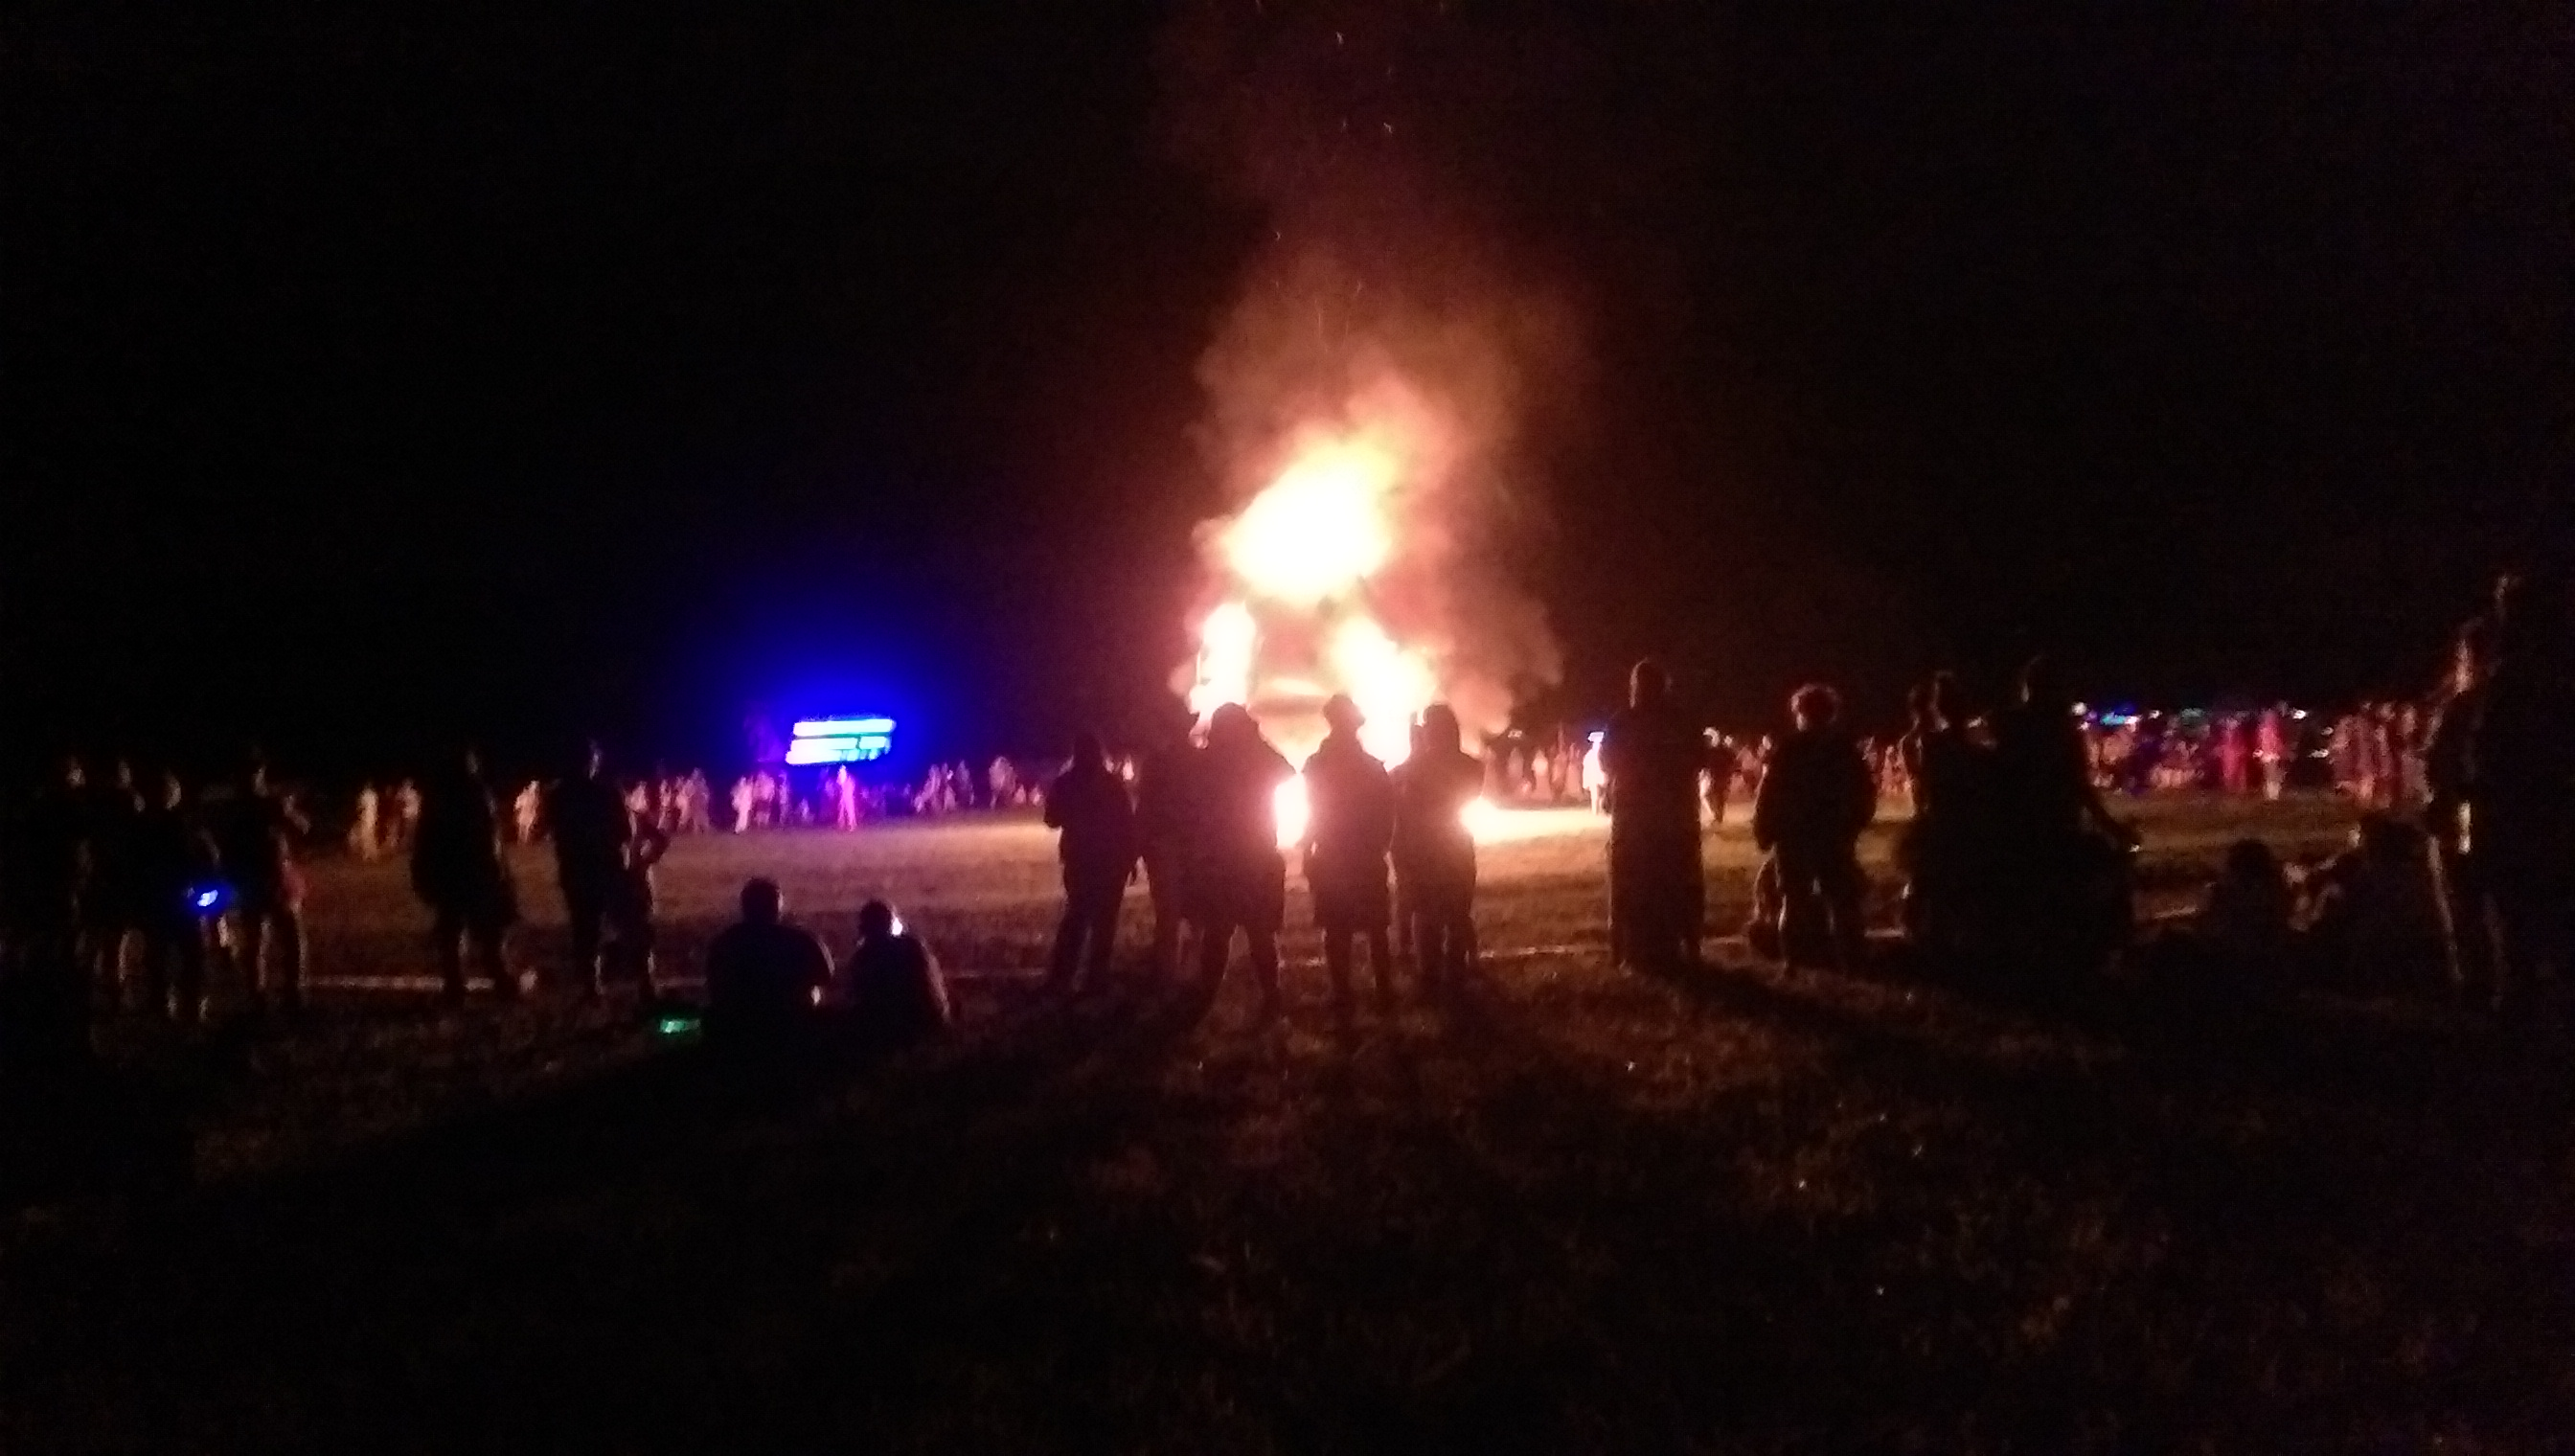
\includegraphics[width=.9\textwidth]{images/TTM2017EffigyBurn}
%     \label{image:2017effigyburn}
% \end{center}
% \vspace*{\fill}



% glossary
\appendix
% \appendixpage
\addappheadtotoc
% \addcontentsline{toc}{chapter}{Appendix}
\chapter[Appendix]{Appendix}
% This is true if only doing the flight manual, not the pre-flight
\ifisflight
  % This one page needs to be one column to look right, even
  % in the flight manual, proper.
  % failed experiment to add thumb guides
%   \addthumb{Welcome}{}{white}{black}
% \putchapterthumb
\fi
% Force printing of all glossary entries, even if not referenced.
% \glsaddall

% \begin{multicols}{2}
\printglossaries
% \end{multicols}

% \vspace*{\fill}
% \begin{center}
% 	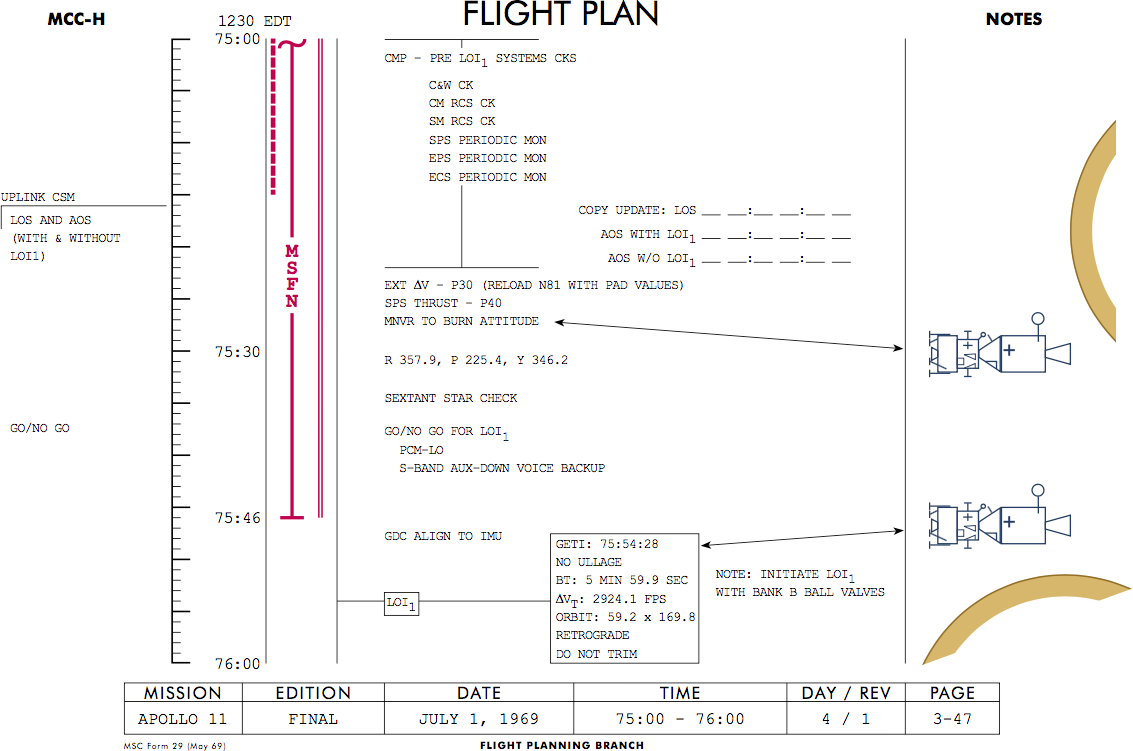
\includegraphics[width=.9\textwidth]{images/flightplan3}
% \end{center}
% \vspace*{\fill}

\ifisflight
\vspace*{\fill}
\begin{figure}[!h]
\centering
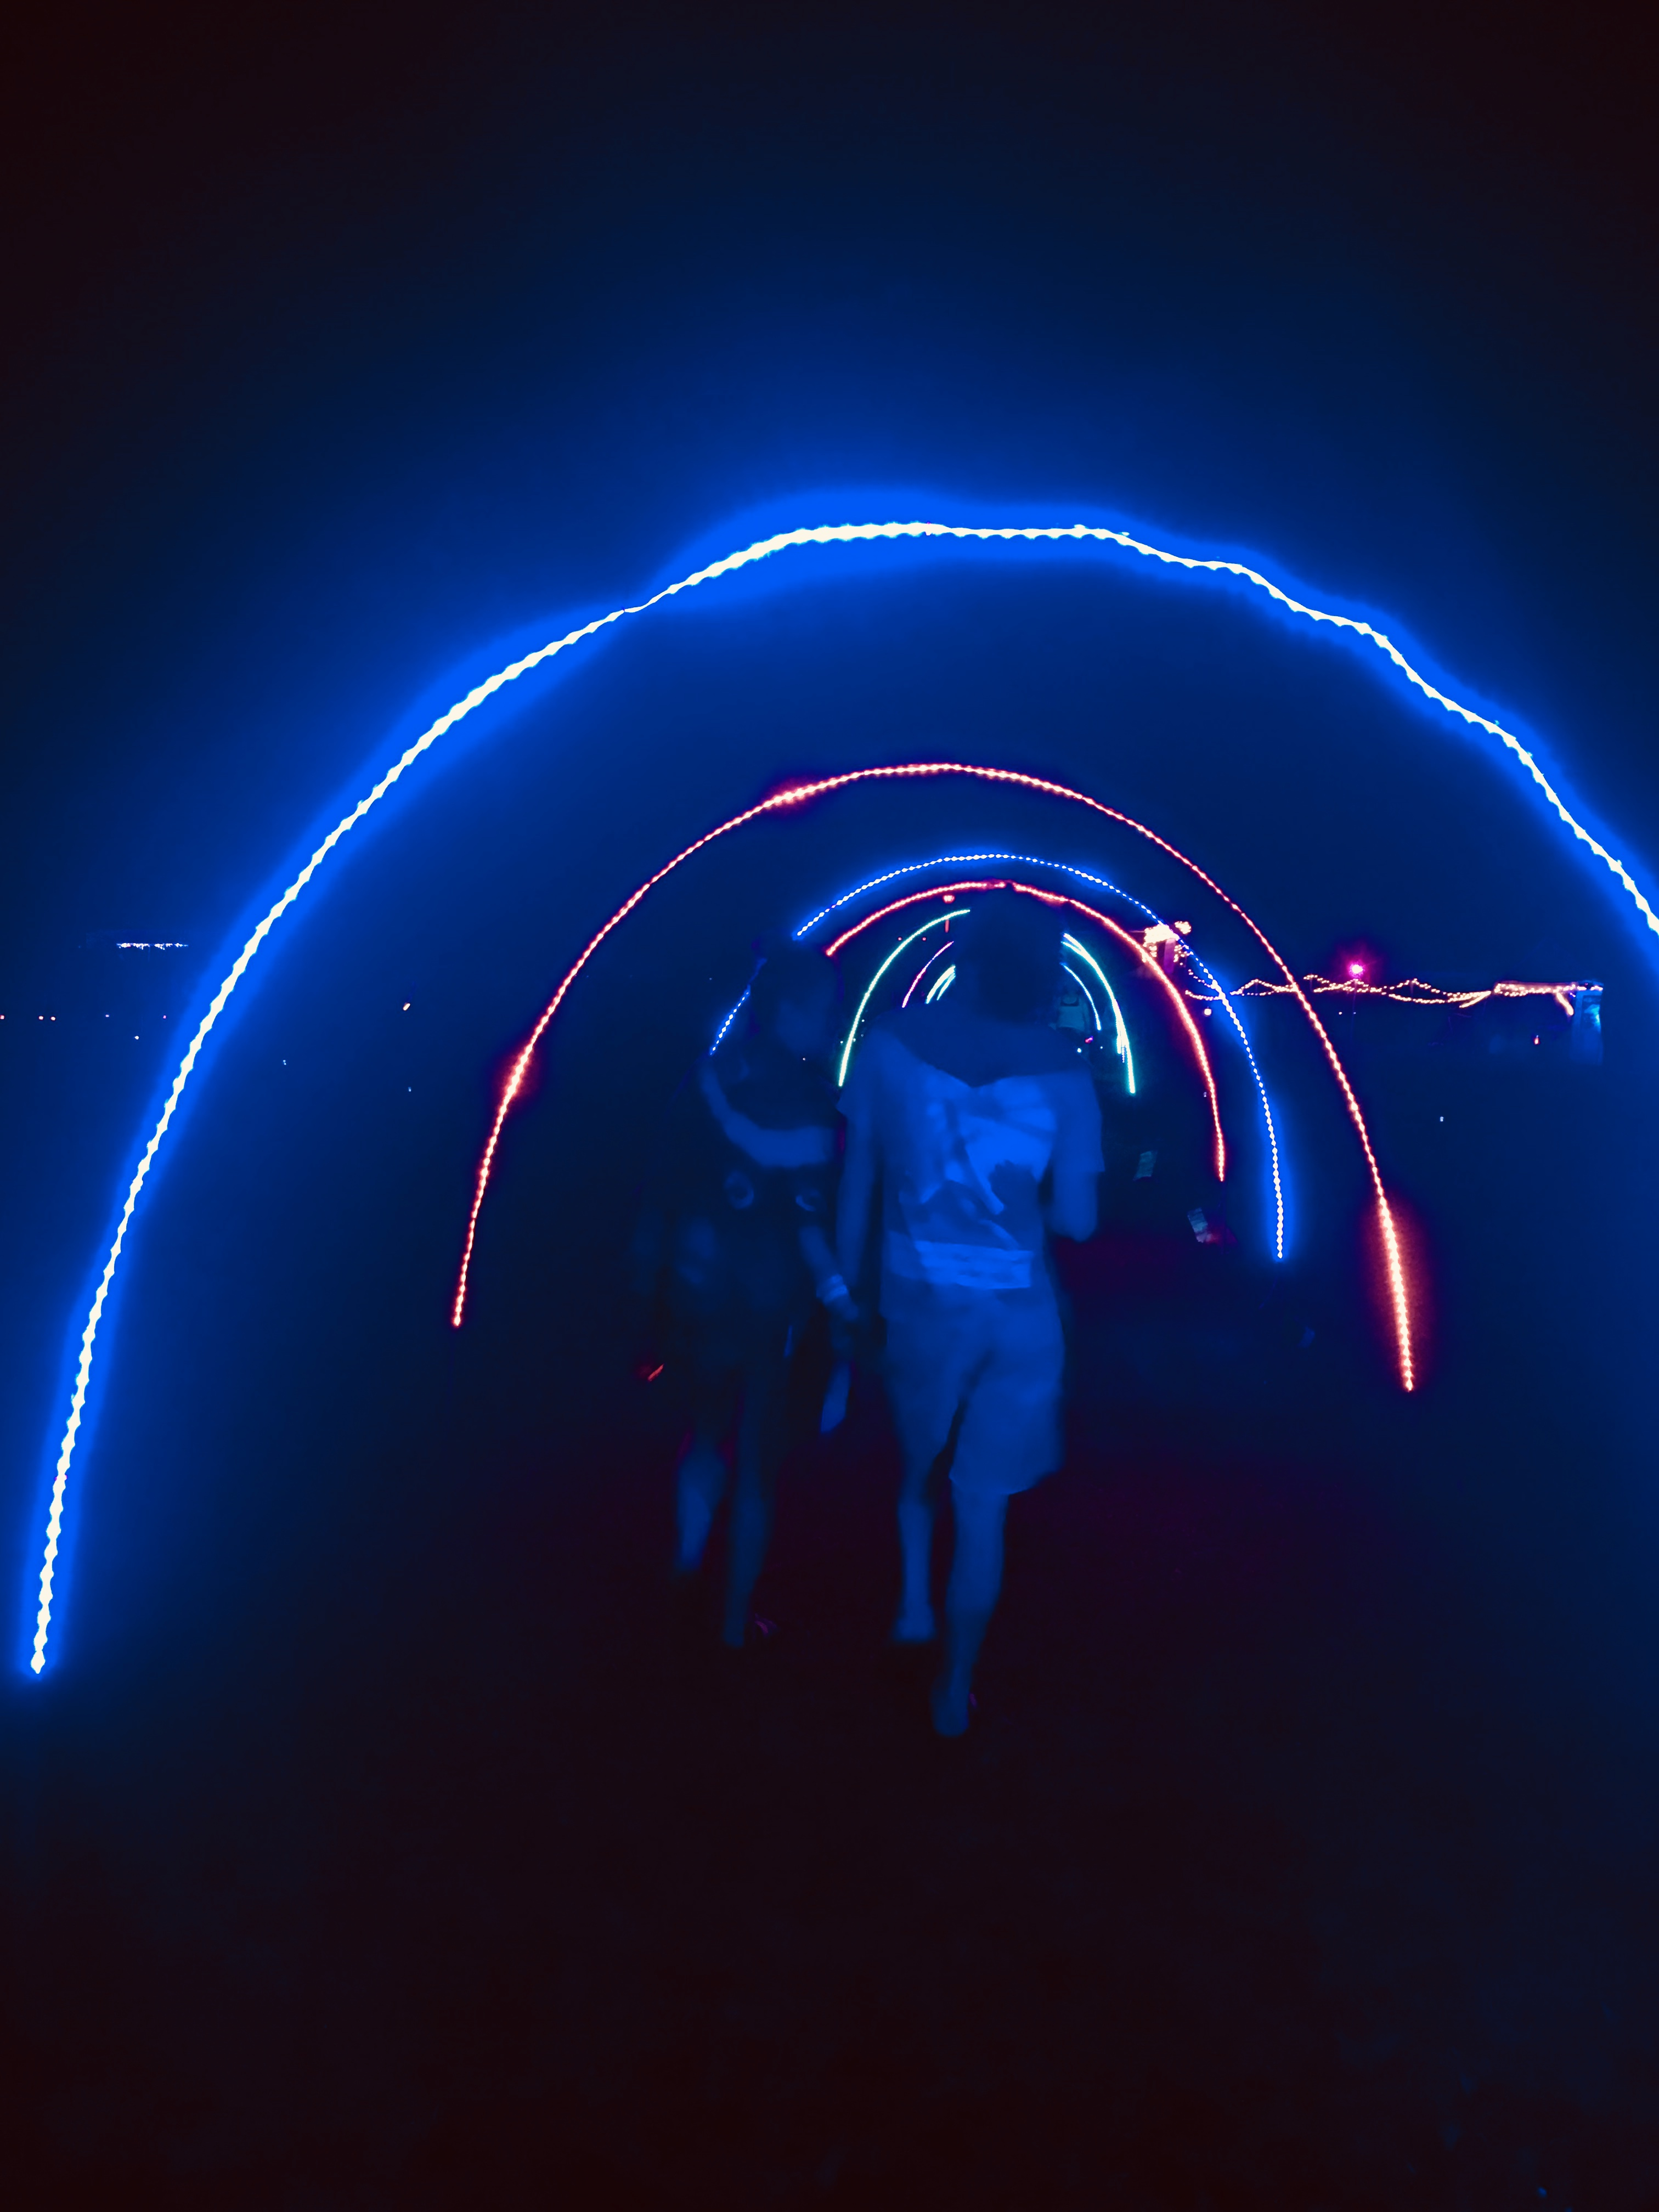
\includegraphics[width=.8\textwidth]{images/TTM2017tunnel.jpeg}
\end{figure}
\vspace*{\fill}

% \clearpage

% \clearpage
% \section*{Notes}

\fi


% \chapter*{Notes}



% % credits
% \chapter{Acknowledgements}
\section*{Image Credits}

% \begin{multicols}{2}
\subsection*{Title Page} 
Andy ``Raptor'' Berres

\subsubsection*{Sources:}
\begin{itemize}[noitemsep]
  \item Galaxy texture: NASA Image Library \url{https://images.nasa.gov/}
  \item Astronaut and moon surface: Project Apollo Archive \url{https://www.flickr.com/photos/projectapolloarchive/}
%   \item Alchemy Element Symbols: public domain
  \item Cat picture: Andy ``Raptor'' Berres
  \item Layout inspiration: Apollo Flight Manual \url{https://www.hq.nasa.gov/alsj/a11/a11fltpln_final_reformat.pdf}
\end{itemize}
\vfill\null

\subsection*{TTM 2018 Artwork}
Thomas O'Connor

\subsection*{Maps}
\begin{description}[leftmargin=6em,noitemsep,style=nextline]
	\item[Direction maps:] Andy ``Raptor'' Berres
	\item[Inside back cover map:] Mark ``Piprrr'' Coletti
\end{description}

\columnbreak



\subsection*{Photos}
\begin{itemize}[noitemsep]
\item Various Apollo Mission photos: Project Apollo Archive \url{https://www.flickr.com/photos/projectapolloarchive/}, NASA
  \item Mountain moon on page \pageref{image:mountainmoom}: \url{https://commons.wikimedia.org/wiki/File:Shenandoah_National_Park_SHEN4850.jpg}
  \item Buzz Aldrin on the Moon on page \pageref{image:buzzaldrin}: \url{https://commons.wikimedia.org/wiki/File:Aldrin_Apollo_11.jpg}
\item 2016 No Swimming at Night sign on page \pageref{fig:2016riversafety}, Judson Hall Photography
\item 2017 Lamplighters on page \pageref{fig:lamplighters2017}, Johnny ``Twaffle'' Benton
\item 2017 Light tunnel on page \pageref{image:tunnel}, Ashley ``Bones'' Maynard
\item 2017 Effigy burn on page \pageref{image:2017effigyburn}, Piprrr
\item Monkey Baker with a Model Jupiter Vehicle on page \pageref{image:missbaker}: \url{https://archive.org/details/MSFC-5909731}
\end{itemize}


\subsection*{Diagrams}
\begin{itemize}[noitemsep]
\item Various Apollo Mission diagrams: Apollo Flight Manual \url{https://www.hq.nasa.gov/alsj/a11/a11fltpln_final_reformat.pdf}
\end{itemize}

\subsection*{Swag}

\begin{description}[leftmargin=6em,noitemsep,style=nextline]
	\item[Design:] Andrea Kerns
  \item[Creation:] Dylan Talley
\end{description}

% \end{multicols}

\clearpage
% We may want to expand this to include all volunteers/leads/co-leads.  Not only
% to acknowledge them ... BUT THIS MEANS A BIGGER HEART!  And we like biggger hearts!

% \topskip0pt
\vspace*{\fill}
\begin{center}
\Large
\textbf{Thank you!}
\end{center}

% \todo[inline]{add photo credits and other tips of the hat}
% We will be adding more and more to this list in the weeks leading up to the event.


\shapepar{\heartshape}
For providing valuable feedback and contributions, the Survival Guide team would like to thank Ben Secrest, Sharon Burdick, Dusty Lashes, Willow Gaia, Kris Long, Andi Glytch, Andrea Kerns, Aley Maurizio, Rebekah Lührs, Abigail Anniemal, Julie Reach,  Katie ``Creamy'' Miller, and Ben ``Cheese Pants'' Bj{\o}st{\aa}d. For their contributions, we would also like to thank all artists, theme camp organizers, and event organizers.  We would also like to thank the Hancock county sherrif's and fire departments for their support.

\bod[inline]{BOD/Teams: who else needs to be acknowledged?}
\vspace*{\fill}

% map and back cover
% \chapter{Site Map}
\section*{Art Index}
\begin{itemize}[itemsep=.0125mm,parsep=2pt]
	\item[\textbf{ 1 }] BAR[ge]
	\item[\textbf{ 2 }] Blacklight Creation Cave
	\item[\textbf{ 3 }] Cafe Burns Misting Station
	\item[\textbf{ 4 }] Comet in stasis
	\item[\textbf{ 5 }] Filia
	\item[\textbf{ 6 }] Gerlach the Friendly Triffid
	\item[\textbf{ 7 }] Hammock City
	\item[\textbf{ 8 }] Kinesios
	\item[\textbf{ 9 }] Lost Temple of Magdaluna
	\item[\textbf{ 10 }] Memento Mori Observatory
	\item[\textbf{ 11 }] MirrorVerse
	\item[\textbf{ 12 }] Moon Shuttles
	\item[\textbf{ 13 }] Pocket Dimension Waystation
	\item[\textbf{ 14 }] Pieces of Us
	\item[\textbf{ 15 }] Pussy Pagoda
	\item[\textbf{ 16 }] River Raft Tie-Off
	\item[\textbf{ 17 }] Tetra Borealis
	\item[\textbf{ 18 }] The Cooler
	\item[\textbf{ 19 }] The Bermuda Pyramid
	\item[\textbf{ 20 }] The Intention Ascension Invention
	\item[\textbf{ 21 }] The Lunar Yearbook
	\item[\textbf{ 22 }] The Moon
	\item[\textbf{ 23 }] The Oracle
	\item[\textbf{ 24 }] The Satin Worshippers Dome
	\item[\textbf{ 25 }] TINY TURTLE CAMP
	\item[\textbf{ 26 }] To The Moon Postcard Photo Frame
	\item[\textbf{ 27 }] Tree Star City
	\item[\textbf{ 28 }] Truffula Tree Grove
	\item[\textbf{ 29 }] Wormhole
	\item[\textbf{ 30 }] You are Water. Our inner Yemaya. 8th Ocean Body
	\item[\textbf{ 31 }] The Visitors Landing Area
	\item[\textbf{ 32 }] Ancient Mysteries Murals
	\item[\textbf{ 33 }] Lunar Fire
	\item[\textbf{ 34 }] Dear Future Me
	\item[\textbf{ 35 }] Zoltar Booth
	\item[\textbf{ 36 }] Lucid Lounge
	\item[\textbf{ 37 }] Gifting Tree
\end{itemize}

\vspace*{\fill}

\section*{Theme Camp Map Index}
\begin{itemize}[itemsep=.0125mm,parsep=2pt]
	\item[\textbf{ 1 }] Acrodesiac Lunartics
	\item[\textbf{ 2 }] Alcoholic Alliterators
	\item[\textbf{ 3 }] As Above So Below
	\item[\textbf{ 4 }] Axis Mundi
	\item[\textbf{ 5 }] Balance
	\item[\textbf{ 6 }] Barefoot Barbaloots
	\item[\textbf{ 7 }] Bazaar Fire Circle
	\item[\textbf{ 8 }] Brownie Brothel
	\item[\textbf{ 9 }] Camp Gargle
	\item[\textbf{ 10 }] Camp Grilled Cheese
	\item[\textbf{ 11 }] Camp Just People
	\item[\textbf{ 12 }] Camp No Friends Here
	\item[\textbf{ 13 }] Camp PFA - Camp
	\item[\textbf{ 14 }] Camp PFA - Lounge
	\item[\textbf{ 15 }] Camp Poor Life Choices
	\item[\textbf{ 16 }] Coffee Camp
	\item[\textbf{ 17 }] Cirque Sur La Lune
	\item[\textbf{ 18 }] Camp Tea and Greet
	\item[\textbf{ 19 }] Department of Synergy
	\item[\textbf{ 20 }] Do It Less Shitty
	\item[\textbf{ 21 }] Dolls to the Wall
	\item[\textbf{ 22 }] Discordia
	\item[\textbf{ 23 }] DRAGon
	\item[\textbf{ 24 }] Glasstaculopolis
	\item[\textbf{ 25 }] Holy Catrimony
	\item[\textbf{ 26 }] HomeSkool
	\item[\textbf{ 27 }] Hippie Haven
	\item[\textbf{ 28 }] Hishersenua
	\item[\textbf{ 29 }] Illumination
	\item[\textbf{ 30 }] InterGalactic Goodies
	\item[\textbf{ 31 }] Interstellar Eggspressions
	\item[\textbf{ 32 }] Interstellar Trill Goats
	\item[\textbf{ 33 }] Kinesios Camping Area
	\item[\textbf{ 34 }] Kind and Kinky
	\newpage
	\item[\textbf{ 35 }] Little Bohemia
	\item[\textbf{ 36 }] Living Dead Room
	\item[\textbf{ 37 }] Martian Playground
	\item[\textbf{ 38 }] McButtStuff Entertainment Emporium
	\item[\textbf{ 39 }] Mermaid Oasis
	\item[\textbf{ 40 }] Made in the Shade
	\item[\textbf{ 41 }] MerBuddah Triangle
	\item[\textbf{ 42 }] Moonspiracy
	\item[\textbf{ 43 }] My Wife's Rack
	\item[\textbf{ 44 }] Neptune Ninjas
	\item[\textbf{ 45 }] Organic Inspiration
	\item[\textbf{ 46 }] Polite As Fuck
	\item[\textbf{ 47 }] Queers Next Door
	\item[\textbf{ 48 }] Renegade Sound
	\item[\textbf{ 49 }] Space Escape
	\item[\textbf{ 50 }] Shameless
	\item[\textbf{ 51 }] Sheriff's Office
	\item[\textbf{ 52 }] Sherwood Moon Base
	\item[\textbf{ 53 }] Spontaneous Combustion
	\item[\textbf{ 54 }] The Bizarre Bazaar
	\item[\textbf{ 55 }] The Black Lodge
	\item[\textbf{ 56 }] The Broken Drum
	\item[\textbf{ 57 }] The Halloweiners
	\item[\textbf{ 58 }] The Tree of Wants \& Whims
	\item[\textbf{ 59 }] Third Aid
	\item[\textbf{ 60 }] Titled Hanger
	\item[\textbf{ 61 }] Unicorn Stampede
	\item[\textbf{ 62 }] We Fuck Loud
	\item[\textbf{ 63 }] We're Occult
	\item[\textbf{ 64 }] Where?House
	\item[\textbf{ 65 }] World Spirits
	\item[\textbf{ 66 }] You Are Beautiful
	\item[\textbf{ 67 }] Zentopia
	\item[\textbf{ 68 }] Temporary Parking/Staging Area
	\item[\textbf{ 69 }] Left Corner Pocket ;) 
\end{itemize}

% \newpage

% \newpage
% \section*{Legend}
% 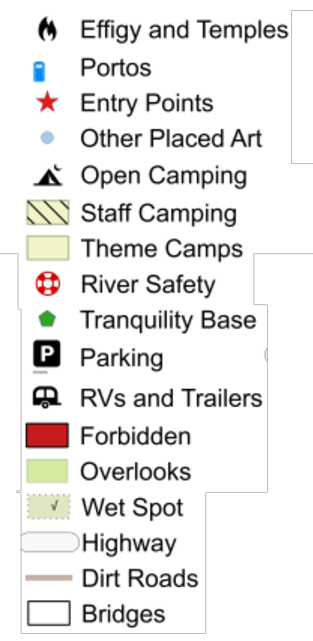
\includegraphics[width=.3\textwidth]{images/Legend_vertical}

% \begin{multicols}{3}
% \begin{itemize}
% \item[] 
\includegraphics[height=8mm]{images/parking} \quad Parking
% \item[] 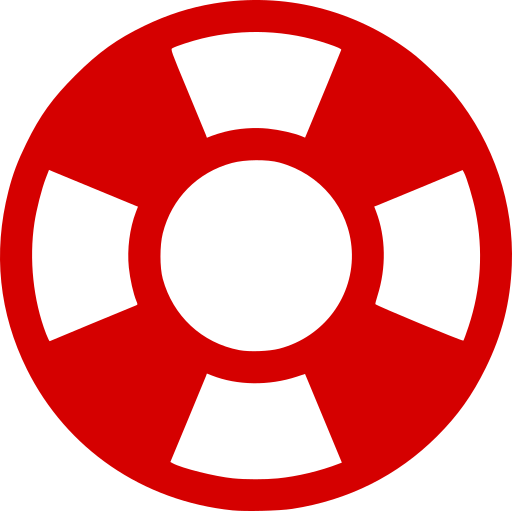
\includegraphics[height=8mm]{images/lifesaver} \quad \parbox[t]{\linewidth-\widthof{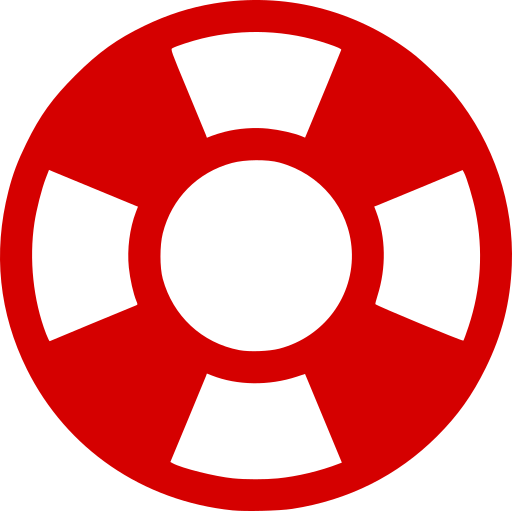
\includegraphics[height=8mm]{images/lifesaver}}}{River Safety\\ Equipment}
% \item[] 
\includegraphics[height=8mm]{images/camper} \quad RV Camping
% \item[] 
\includegraphics[height=8mm]{images/camping} \quad Open Camping
% \item[] 
\includegraphics[height=8mm]{images/portapotty} \quad Port-a-Potty
% \end{itemize}

% \end{multicols}

% \begin{tabular}{llllll}
% 
\includegraphics[height=8mm]{images/parking} & Parking & 
% 
\includegraphics[height=8mm]{images/camper} & RV Camping & 
% 
\includegraphics[height=8mm]{images/portapotty} & Port-a-Potty \\
% 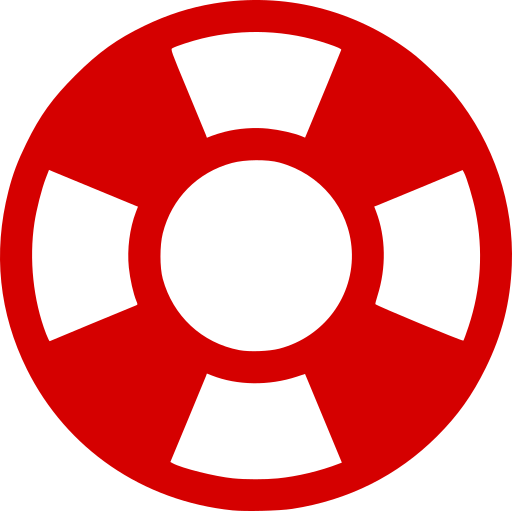
\includegraphics[height=8mm]{images/lifesaver} & \parbox[t]{3cm}{River Safety \\Equipment} & 
% 
\includegraphics[height=8mm]{images/camping} & Open Camping  
% &  & 
% \end{tabular}

%
% map.tex
%
% Contains the TTM map

\clearpage
\section*{Art}
\vspace*{\fill}
\begin{center}
	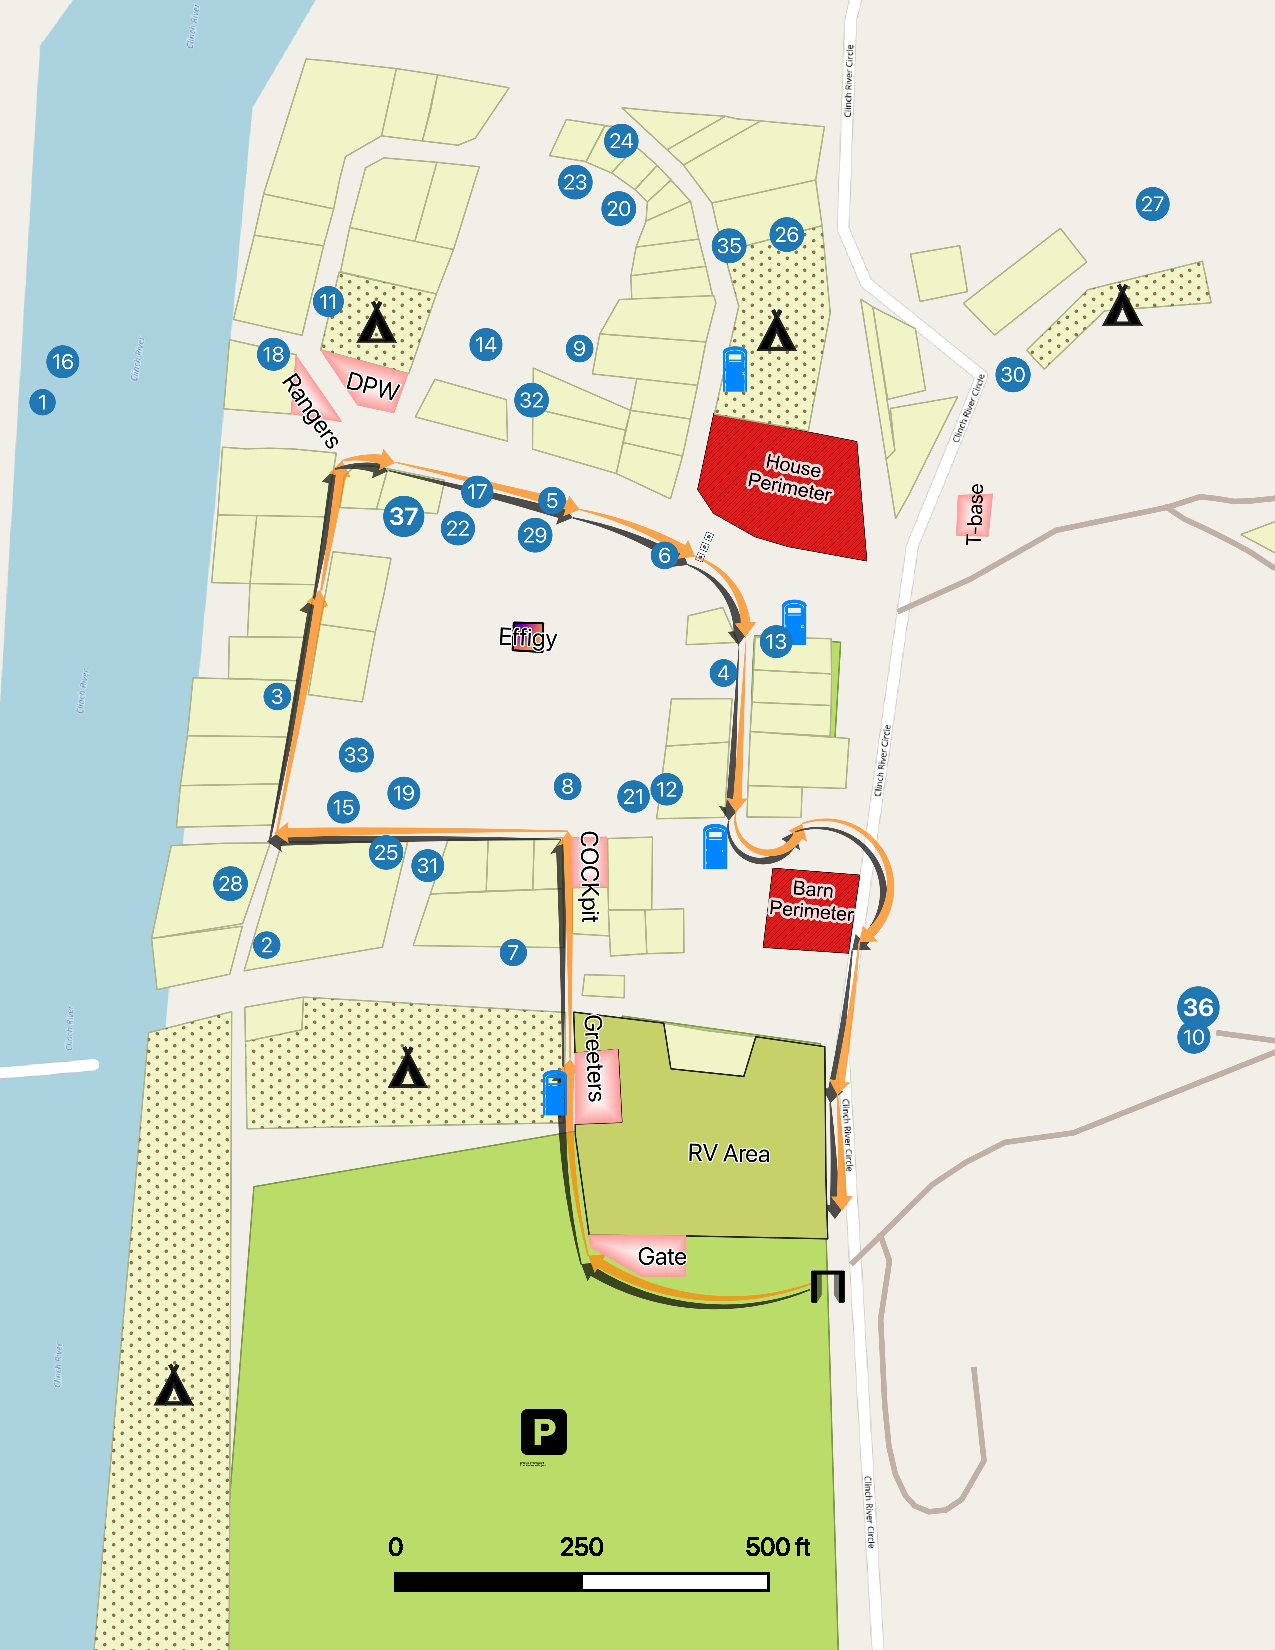
\includegraphics[width=.95\textwidth]{images/2019TTMArt}
\end{center}
\vspace*{\fill}

\clearpage
\section*{Theme Camps}
\vspace*{\fill}
\begin{center}
	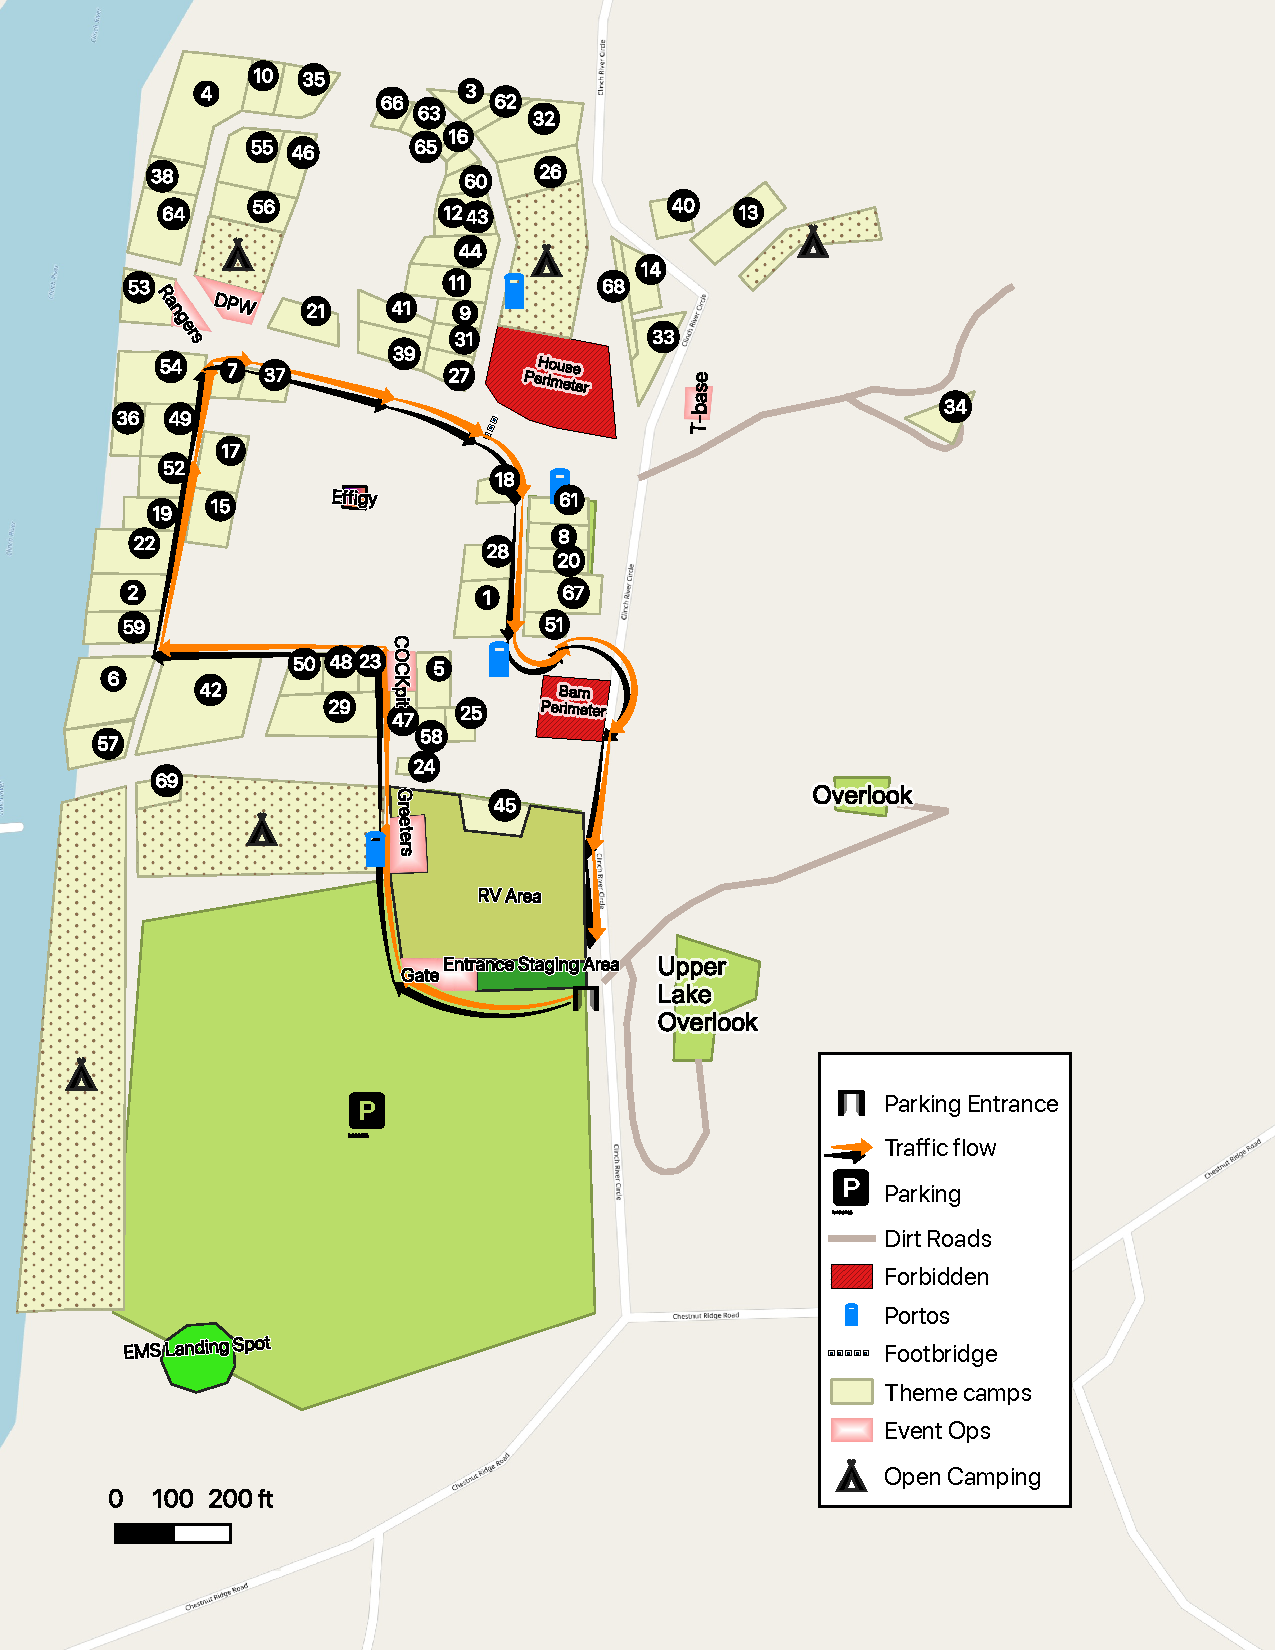
\includegraphics[width=.95\textwidth]{images/TTM2019Pocket}
\end{center}
\vspace*{\fill}

% %
% backcover.tex
%
% This is the outside back cover graphic
%


% We want this to be the back cover
\clearpage
\thispagestyle{empty}
\begin{figure}[h!]
	\centering
	
\includegraphics[angle=90,width=\textwidth]{images/TTM2018_smaller}
    \small
    (Artwork courtesy Thomas O'Connor)
\end{figure}



\end{document}
